%% LyX 2.3.6.1 created this file.  For more info, see http://www.lyx.org/.
%% Do not edit unless you really know what you are doing.
\documentclass[11pt,oneside,american,czech]{book}


\usepackage[T1]{fontenc}
% \usepackage[IL2]{fontenc}
\usepackage[utf8]{inputenc}
\usepackage[a4paper]{geometry}
\usepackage[czech]{babel}


% \usepackage[cp1250]{inputenc}
\geometry{verbose,tmargin=4cm,bmargin=3cm,lmargin=3cm,rmargin=2cm,headheight=0.8cm,headsep=1cm,footskip=1cm} 
\pagestyle{headings}
\setcounter{secnumdepth}{3}
\usepackage{url}
\usepackage{amsmath}
\usepackage{amsthm}
\usepackage{amssymb}
\usepackage{graphicx}
\usepackage{setspace}
\usepackage{float}
\usepackage{tcolorbox}
\usepackage{multicol}
\usepackage{subcaption}
\usepackage[export]{adjustbox}
\usepackage{xcolor}
\usepackage{listings}
\usepackage{xparse}
\usepackage{mathtools}
\usepackage{booktabs}

\usepackage{svg}



\colorlet{light-gray}{gray!20}
\definecolor{codegray}{rgb}{0.5,0.5,0.5}


\lstset{language=C++,keywordstyle={\bfseries \color{blue}}}


\newcommand*\Laplace{\mathop{}\!\mathbin\bigtriangleup}



\makeatletter
%%%%%%%%%%%%%%%%%%%%%%%%%%%%%% Textclass specific LaTeX commands.
\newenvironment{lyxlist}[1]
	{\begin{list}{}
		{\settowidth{\labelwidth}{#1}
		 \setlength{\leftmargin}{\labelwidth}
		 \addtolength{\leftmargin}{\labelsep}
		 \renewcommand{\makelabel}[1]{##1\hfil}}}
	{\end{list}}

%%%%%%%%%%%%%%%%%%%%%%%%%%%%%% User specified LaTeX commands.
%% Font setup: please leave the LyX font settings all set to 'default'
%% if you want to use any of these packages:

%% Use Times New Roman font for text and Belleek font for math
%% Please make sure that the 'esint' package is turned off in the
%% 'Math options' page.
\usepackage[varg]{txfonts}

%% Use Utopia text with Fourier-GUTenberg math
%\usepackage{fourier}

%% Bitstream Charter text with Math Design math
%\usepackage[charter]{mathdesign}

%%---------------------------------------------------------------------

%% Make the multiline figure/table captions indent so that the second
%% line "hangs" right below the first one.
%\usepackage[format=hang]{caption}

%% Indent even the first paragraph in each section
\usepackage{indentfirst}

%%---------------------------------------------------------------------

%% Disable page numbers in the TOC. LOF, LOT (TOC automatically
%% adds \thispagestyle{chapter} if not overriden
%\addtocontents{toc}{\protect\thispagestyle{empty}}
%\addtocontents{lof}{\protect\thispagestyle{empty}}
%\addtocontents{lot}{\protect\thispagestyle{empty}}

%% Shifts the top line of the TOC (not the title) 1cm upwards 
%% so that the whole TOC fits on 1 page. Additional page size
%% adjustment is performed at the point where the TOC
%% is inserted.
%\addtocontents{toc}{\protect\vspace{-1cm}}

%%---------------------------------------------------------------------

% completely avoid orphans (first lines of a new paragraph on the bottom of a page)
\clubpenalty=9500

% completely avoid widows (last lines of paragraph on a new page)
\widowpenalty=9500

% disable hyphenation of acronyms
\hyphenation{CDFA HARDI HiPPIES IKEM InterTrack MEGIDDO MIMD MPFA DICOM ASCLEPIOS MedInria}

%%---------------------------------------------------------------------

%% Print out all vectors in bold type instead of printing an arrow above them
\renewcommand{\vec}[1]{\boldsymbol{#1}}

% Replace standard \cite by the parenthetical variant \citep
%\renewcommand{\cite}{\citep}

\makeatother


\usepackage{afterpage}

\usepackage{todonotes}

\usepackage{hyperref}

\usepackage{comment}

    

\newcommand{\nazevcz}{Numerick\'{y} model neizoterm\'{a}ln\'{\i}ho proud\v{e}n\'{\i} a obt\'{e}k\'{a}n\'{\i} p\v{r}ek\'{a}\v{z}ek zalo\v{z}en\'{y} na m\v{r}\'{\i}\v{z}kov\'{e} Boltzmannov\v{e} metod\v{e}}

\newcommand{\nazeven}{Numerical model of non-isothermal flow around obstacles based on the lattice Boltzmann method}

\newcommand{\skola}{\cvut}
\newcommand{\fakulta}{\fjfi}
\newcommand{\katedra}{\km}
\newcommand{\kde}{Praze} 
\newcommand{\program}{Aplikace přírodních věd} 
\newcommand{\obor}{Matematické inženýrství}
\newcommand{\zamereni}{Matematické modelování}

\newcommand{\autor}{Bc. Dominik Horák}


\newcommand{\vedouci}{doc. Ing. Radek Fučík Ph.D.}
\newcommand{\pracovisteVed}{Katedra matematiky, Fakulta jaderná a fyzikálně inženýrská, České vysoké učení technické v Praze, Trojanova 13, 120 00, Praha 2}

\newcommand{\konzultant}{Ing. Jakub Klinkovsk\'{y} Ph.D.}
\newcommand{\pracovisteKonz}{Scuderia AlphaTauri S.p.A., Via Boaria 229, 48018 Faenza (RA), Itálie}


\newcommand{\blankpage}
{   \null
    \thispagestyle{empty}%
    \newpage}

\usepackage{pdfpages}

\makeatletter
\newcommand{\vast}{\bBigg@{4}}
\newcommand{\Vast}{\bBigg@{5}}

\begin{document}
\def\documentdate{7. \v{c}ervence 2023}

%%\def\documentdate{\today}

\pagestyle{empty}
{\centering

\noindent %
\begin{minipage}[c]{3cm}%
\noindent \begin{center}
\includegraphics[width=3cm,height=3cm,keepaspectratio]{Img/TITLE/cvut}
\par\end{center}%
\end{minipage}%
\begin{minipage}[c]{0.6\linewidth}%
\begin{center}
\textsc{\large{}České vysoké učení technické v Praze}{\large{}}\\
{\large{}Fakulta jaderná a fyzikálně inženýrská}
\par\end{center}%
\end{minipage}%
\begin{minipage}[c]{3cm}%
\noindent \begin{center}
\includegraphics[width=3cm,height=3cm,keepaspectratio]{Img/TITLE/fjfi}
\par\end{center}%
\end{minipage}

\vspace{3cm}

\textbf{\huge{}\nazevcz
}{\huge\par}

\vspace{1cm}

\selectlanguage{american}%
\textbf{\huge{}\nazeven}{\huge\par}

\selectlanguage{czech}%
\vspace{2cm}

{\large{}Diplomov\'{a} pr\'{a}ce\large\par}

}

\vfill{}

\begin{lyxlist}{MMMMMMMMM}
\begin{singlespace}
\item [{Autor:}] \textbf{\autor}
\item [{Vedoucí~práce:}] \textbf{\konzultant}
\item [{Konzultant:}] \textbf{\vedouci}
\item [{Akademický~rok:}] 2023/2024
\end{singlespace}
\end{lyxlist}

\afterpage{\blankpage}





% \includepdf[pages=1]{Img/PredniZadani.pdf}

% \includepdf[pages=1]{Img/ZadniZadani.pdf}


\noindent \emph{\Large{}Pod\v{e}kov\'{a}n\'{\i}:}{\Large\par}

\noindent Cht\v{e}l bych zde pod\v{e}kovat p\v{r}edev\v{s}\'{\i}m m\'{y}m vedouc\'{\i}m Ing. Jakubovi Klinkovsk\'{e}mu Ph.D. a doc. Ing. Radku Fu\v{c}\'{\i}kovi, Ph.D. za ochotu, z\'{a}zem\'{\i}, pe\v{c}livost a v neposledn\'{\i} \v{r}ad\v{e} tak\'{e} za neoceniteln\'{e} rady bez kter\'{y}ch by tato pr\'{a}ce nevznikla. M\'{e} d\'{\i}ky pat\v{r}\'{\i} tak\'{e} m\'{e} rodin\v{e} a p\v{r}\'{\i}telkyni za ve\v{s}kerou podporu p\v{r}i studiu.

Tato pr\'{a}ce byla podpo\v{r}ena grantem Studentsk\'{e} grantov\'{e} sout\v{e}\v{z}e \v{C}VUT \v{c}. SGS20/184/OHK4/3T/14.

\vfill

\noindent \emph{\Large{}Čestné prohlášení:}{\Large\par}

\noindent Prohlašuji, že jsem tuto práci vypracoval samostatně a uvedl
jsem všechnu použitou literaturu.

\bigskip{}

\noindent V Praze dne 10. kv\v{e}tna 2024 \hfill{}\autor

\vspace{2cm}

\pagestyle{empty}

\afterpage{\blankpage}
\newpage{}

\begin{onehalfspace}
\noindent \emph{Název práce:}

\noindent \textbf{\nazevcz}
\end{onehalfspace}

\bigskip{}

\noindent \emph{Autor:} \autor

\bigskip{}

\noindent \emph{Obor:} \obor\bigskip{}

\noindent \emph{Zaměření:} \zamereni

\bigskip{}

\noindent \emph{Druh práce:} V\'{y}zkumn\'{y} \'{u}kol

\bigskip{}

\noindent \emph{Vedoucí práce:} \vedouci, \pracovisteVed

\bigskip{}

\noindent \emph{Konzultant:} \konzultant, \pracovisteVed

\bigskip{}

\noindent \emph{Abstrakt:} Pr\'{a}ce se zab\'{y}v\'{a} matematick\'{y}m modelov\'{a}n\'{i}m neizoterm\'{a}ln\'{i}ho proud\v{e}n\'{\i} nestla\v{c}iteln\'{e} Newtonovsk\'{e} tekutiny. Pr\'{a}ce si klade za c\'{\i}l implementovat a popsat p\v{r}estup tepla ve 3D numerick\'{e}m modelu. V teoretick\'{e} \v{c}\'{a}sti je prezentov\'{a}n matematick\'{y} model neizoterm\'{a}ln\'{\i}ho proud\v{e}n\'{i} Newtonovsk\'{e} tekutiny spolu se z\'{a}kladn\'{\i}m popisem chlad\'{i}c\'{i}ho okruhu studentsk\'{e} formule. Ve druh\'{e} \v{c}\'{a}sti je \v{c}ten\'{a}\v{r} sezn\'{a}men s m\v{r}\'{\i}\v{z}kovou Boltzmannovou metodou (LBM) a posledn\'{i} \v{c}\'{a}st je pak v\v{e}nov\'{a}na diskuzi v\'{y}sledk\r{u} aplikace LBM s implementovan\'{y}m p\v{r}estupem tepla na matematick\'{y} model. Implementace p\v{r}estupu teploty byla \'{u}sp\v{e}\v{s}n\'{a} a metoda produkuje uspokojiv\'{e} v\'{y}sledky.




\bigskip{}

\noindent \emph{Klíčová slova:} mřížková Boltzmannova metoda, MPI, rovnice veden\'{\i} tepla, simulace proudění na GPU

\vfill{}
~

\selectlanguage{american}%
\begin{onehalfspace}
\noindent \emph{Title:}

\noindent \textbf{\nazeven}
\end{onehalfspace}

\bigskip{}

\noindent \emph{Author:} \autor

\bigskip{}

\noindent \emph{Abstract:} The work deals with the mathematical modeling of non-isothermal flow of incompressible Newtonian fluids. The aim of the work is to implement and describe heat transfer in a 3D numerical model. In the theoretical part, the mathematical model of non-isothermal flow of Newtonian fluids is presented together with a basic description of the cooling circuit of a student formula car. In the second part, the reader is introduced to the lattice Boltzmann method (LBM), and the last part discusses the results of the application of LBM with implemented heat transfer to the mathematical model. The implementation of heat transfer was successful, and the method produces satisfactory results.

\bigskip{}

\noindent \emph{Key words:} lattice Boltzmann method, MPI, heat equation, flow simulation on GPU


\selectlanguage{czech}%
\newpage{}

\pagestyle{headings}

\tableofcontents{}

\newpage{}

\chapter*{\'{U}vod}

\addcontentsline{toc}{chapter}{\'{U}vod}

    Tato pr\'{a}ce se zab\'{y}v\'{a} problematikou simulace proud\v{e}n\'{\i} tekutin (anglicky computational fluid dynamics, d\'{a}le CFD), za pou\v{z}it\'{\i} m\v{r}\'{\i}\v{z}kov\'{e} Boltzmannovy metody (LBM), co\v{z} pat\v{r}\'{\i} mezi nejsklonovan\v{e}j\v{s}\'{\i} t\'{e}mata na poli numerick\'{e} matematiky. Z\'{a}rove\v{n} je CFD velmi hojn\v{e} vyu\v{z}\'{\i}van\'{e} v praxi, nap\v{r}\'{\i}klad ve Formuli 1. V automobilov\'{e}m pr\r{u}myslu obecn\v{e} je v posledn\'{\i}ch letech st\'{a}le v\v{e}t\v{s}\'{\i} d\r{u}raz kladen na numerick\'{e} simulace narozd\'{\i}l od experiment\r{u}, kter\'{e} b\'{y}vaj\'{\i} finan\v{c}n\v{e} mnohem n\'{a}ro\v{c}n\v{e}j\v{s}\'{\i}.

    V p\v{r}edch\'{a}zej\'{\i}c\'{\i} bakal\'{a}\v{r}sk\'{e} pr\'{a}ci \cite{BP_DH} bylo zkoum\'{a}no neizoterm\'{a}ln\'{\i} proud\v{e}n\'{\i} okolo p\v{r}ek\'{a}\v{z}ek a spolu s n\'{\i}m i aerodynamick\'{e} vlastnosti tohoto proud\v{e}n\'{\i}. V t\'{e}to pr\'{a}ci je hlavn\'{\i}m c\'{\i}lem simulovat izoterm\'{a}ln\'{\i} proud\v{e}n\'{\i} spolu s p\v{r}estupem tepla mezi r\r{u}zn\'{y}mi typy prost\v{r}ed\'{\i}.

    % V r\'{a}mci t\'{e}to pr\'{a}ce byla nav\'{a}z\'{a}na spolupr\'{a}ce s t\'{y}mem eForce FEE Prague Formula \cite{eForce_FS}, kter\'{y} p\r{u}sob\'{\i} v studentsk\'{e} sout\v{e}\v{z}i Formula Student \cite{FS} s elektrickou formul\'{\i}. C\'{\i}lem sout\v{e}\v{z}e je postavit z\'{a}vodn\'{\i} auto, ale nen\'{\i} to pouze o v\'{y}konu -- hodnot\'{\i} se tak\'{e} konstrukce, pl\'{a}nov\'{a}n\'{\i} rozpo\v{c}tu i marketingov\'{y} pl\'{a}n. V p\v{r}\'{\i}pad\v{e} pou\v{z}it\'{\i} CFD pro izoterm\'{a}ln\'{\i}ho proud\v{e}n\'{\i} se nab\'{\i}z\'{\i} zkoum\'{a}n\'{\i} chlad\'{\i}c\'{\i}ho okruhu popsan\'{e}ho v t\'{e}to pr\'{a}ci. Tato pr\'{a}ce se zam\v{e}\v{r}uje v\'{y}hradn\v{e} na samotn\'{y} radi\'{a}tor neboli v\'{y}m\v{e}n\'{\i}k tepla.

    Pr\'{a}ce je rozd\v{e}lena do \v{c}ty\v{r} kapitol. V prvn\'{\i} kapitole je p\v{r}edstaven matematick\'{y} model dynamiky tekutin 
    formulac\'{\i} \'{u}lohy. 
    
    Ve druh\'{e} kapitole je \v{c}ten\'{a}\v{r} sezn\'{a}men s m\v{r}\'{\i}\v{z}kovou Boltzmannovou metodou. Pops\'{a}ny jsou z\'{a}kladn\'{\i} principy metody, numerick\'{a} sch\'{e}mata pou\v{z}\'{\i}van\'{a} p\v{r}i simulac\'{\i}ch, spolu s p\v{r}edstaven\'{\i}m okrajov\'{y}ch podm\'{\i}nek a algoritmu LBM.
    V t\'{e}to kapitole je tak\'{e} pops\'{a}na p\v{r}estupov\'{a} okrajov\'{a} podm\'{\i}nka implementovan\'{a} v r\'{a}mci t\'{e}to pr\'{a}ce. 
    
    T\v{r}et\'{\i} kapitola je v\v{e}nov\'{a}na pozn\'{a}mk\'{a}m k implementaci k\'{o}du

    D\'{a}le zde \v{c}ten\'{a}\v{r} nalezne popis datov\'{y}ch struktur pou\v{z}it\'{y}ch k implementaci LBM. V posledn\'{\i} kapitole jsou prezentov\'{a}ny v\'{y}sledky aplikace m\v{r}\'{\i}\v{z}kov\'{e} Boltzmannovy metody na matematick\'{y} model zaveden\'{y} v prvn\'{\i} kapitole. V t\'{e}to \v{c}\'{a}sti je nejprve komentov\'{a}na implementace pole pro r\r{u}zn\'{e} difuzn\'{\i} koeficienty, d\'{a}le je zde ov\v{e}\v{r}ov\'{a}na p\v{r}estupov\'{a} okrajov\'{a} podm\'{\i}nka a hled\'{a}ny optim\'{a}ln\'{\i} rozm\v{e}ry chladi\v{c}e. Na z\'{a}v\v{e}r t\'{e}to kapitoly jsou diskutov\'{a}na mo\v{z}n\'{e} sm\v{e}ry dal\v{s}\'{\i}ho zlep\v{s}en\'{\i} modelu.

    Ke zm\'{\i}n\v{e}n\'{y}m numerick\'{y}m simulac\'{\i}m byl vyu\v{z}\'{\i}v\'{a}n k\'{o}d LBM vyv\'{\i}jen\'{y} ji\v{z} n\v{e}kolik let na KM FJFI \v{C}VUT v Praze. K\'{o}d je naps\'{a}n v jazyce C++ a je v n\v{e}m vyu\v{z}ita architektura CUDA umo\v{z}\v{n}uj\'{\i}c\'{\i} paraleln\'{\i} po\v{c}\'{\i}t\'{a}n\'{\i} na grafick\'{y}ch kart\'{a}ch. D\'{a}le k\'{o}d vyu\v{z}\'{\i}v\'{a} knihovny OpenMPI pro paraleln\'{\i} po\v{c}\'{\i}t\'{a}n\'{\i} na v\'{\i}ce grafick\'{y}ch kart\'{a}ch. V\'{y}po\v{c}ty byly prim\'{a}rn\v{e} uskute\v{c}n\v{e}ny na v\'{y}po\v{c}etn\'{\i}m clusteru HELIOS na KM FJFI \v{C}VUT, konkr\'{e}tn\v{e} na grafick\'{y}ch kart\'{a}ch NVIDIA A100 s 80 GB pam\v{e}t\'{\i}. D\'{\i}ky funkcionalit\v{e} OpenMPI bylo mo\v{z}n\'{e} vyu\v{z}\'{\i}t v\v{s}echny \v{c}ty\v{r}i dostupn\'{e} grafick\'{e} karty najednou. Tento k\'{o}d byl n\'{a}sledn\v{e} modifikov\'{a}n dle pot\v{r}eb zad\'{a}n\'{\i} -- byla do n\v{e}j implementov\'{a}na p\v{r}estupov\'{a} okrajov\'{a} podm\'{\i}nka a d\'{a}le bylo p\v{r}id\'{a}no difuzn\'{\i} pole umo\v{z}\v{n}uj\'{\i}c\'{\i} nastaven\'{\i} odli\v{s}n\'{e}ho difuzn\'{\i}ho koeficientu pro r\r{u}zn\'{e} objekty v simulaci. 

    % Tato práce se zab\'{y}v\'{a} problematikou simulace proud\v{e}n\'{\i} tekutin (z anglick\'{e}ho computational fluid dynamics, d\'{a}le CFD), co\v{z} je jedno z nejv\'{\i}ce zkouman\'{y}ch odv\v{e}tv\'{\i} numerick\'{e} matematiky a z\'{a}rove\v{n} intenzivn\v{e} vyu\v{z}\'{\i}van\'{e} v praxi, nap\v{r}\'{\i}klad ve Formuli 1. Ve zm\'{\i}n\v{e}n\'{e}m motorsportu, ale i automobilov\'{e}m pr\r{u}myslu obecn\v{e}, jsou n\'{a}klady spojen\'{e} s optimalizac\'{\i} voz\r{u} vysok\'{e}. Nejen proto jsou st\'{a}le v\'{\i}ce experiment\'{a}ln\'{\i} modely v ran\'{y}ch f\'{a}z\'{\i}ch projekt\r{u} nahrazov\'{a}ny numerick\'{y}mi simulacemi. Mezi dal\v{s}\'{\i} v\'{y}hody numerick\'{y}ch simulac\'{\i} pat\v{r}\'{\i} mo\v{z}nost snadno je pozm\v{e}nit na jednotliv\'{e} \'{u}lohy.

    % Numerick\'{a} metoda studovan\'{a} v této bakalářské pr\'{a}ci je m\v{r}\'{\i}\v{z}kov\'{a} Boltzmannova metoda (LBM, z~anglick\'{e}ho Lattice-Boltzmann method) vyvinut\'{a} na p\v{r}elomu 80. a 90. let dvac\'{a}t\'{e}ho stolet\'{\i}. D\'{\i}ky mo\v{z}nosti paraleln\'{\i}ch v\'{y}po\v{c}t\r{u} na GPU t\v{e}\v{s}\'{\i} se tato metoda rozmachu hlavn\v{e} v posledn\'{\i}ch patn\'{a}cti letech, kdy jsou na trhu rok od roku v\'{y}konn\v{e}j\v{s}\'{\i} grafick\'{e} karty umo\v{z}\v{n}uj\'{\i}c\'{\i} st\'{a}le n\'{a}ro\v{c}n\v{e}j\v{s}\'{\i} v\'{y}po\v{c}ty. C\'{\i}lem t\'{e}to pr\'{a}ce je kr\'{a}tce nahl\'{e}dnout do problematiky aplikace LBM na simulaci proud\v{e}n\'{\i} tekutiny okolo p\v{r}ek\'{a}\v{z}ky. 

    
    % K numerick\'{y}m simulac\'{\i}m byl vyu\v{z}\'{\i}v\'{a}n k\'{o}d LBM napsan\'{y} v jazyce C++, kter\'{y} je ji\v{z} n\v{e}kolik let vyv\'{\i}jen\'{y} na KM FJFI \v{C}VUT v Praze. K\'{o}d vyu\v{z}\'{\i}v\'{a} softwarov\'{e} architektury CUDA, kter\'{a} umo\v{z}\v{n}uje paraleln\'{\i} v\'{y}po\v{c}y na grafick\'{y}ch kart\'{a}ch. Tento k\'{o}d byl modifikov\'{a}n dle pot\v{r}eb zad\'{a}n\'{\i} pr\'{a}ce, zejm\'{e}na v~n\v{e}m byla implementov\'{a}na metoda v\'{y}m\v{e}ny hybnosti pro v\'{y}po\v{c}et s\'{\i}ly p\r{u}sob\'{\i}c\'{\i} na t\v{e}leso p\v{r}i obt\'{e}k\'{a}n\'{\i}, s \v{c}\'{\i}m\v{z} souvis\'{\i} i v\'{y}po\v{c}et bezrozm\v{e}rn\'{y}ch koeficient\r{u}. Pro implementaci metody v\'{y}m\v{e}ny hybnosti bylo nejprve nutn\'{e} na grafick\'{e} kart\v{e} rozd\v{e}lit v\'{y}po\v{c}et kolize a \v{s}\'{\i}\v{r}en\'{\i}, abychom z\'{\i}skali spr\'{a}vn\'{e} hodnoty k~v\'{y}po\v{c}tu s\'{\i}ly. D\'{a}le se v r\'{a}mci t\'{e}to pr\'{a}ce poda\v{r}ilo roz\v{s}\'{\i}\v{r}it SDL o ukazatel fluktuac\'{\i} v re\'{a}ln\'{e}m \v{c}ase.
    
    % Pr\'{a}ce je rozd\v{e}lena do t\v{r}\'{\i} kapitol. Nejprve se \v{c}ten\'{a}\v{r} sezn\'{a}m\'{\i} s matematick\'{y}m modelem dynamiky tekutin, z\'{a}kladn\'{\i}mi pojmy z aerodynamiky a formulac\'{\i} \'{u}lohy, v dal\v{s}\'{\i} \v{c}\'{a}sti je p\v{r}edstavena m\v{r}\'{\i}\v{z}kov\'{a} Boltzmannova metoda pou\v{z}it\'{a} p\v{r}i numerick\'{y}ch simulac\'{\i}ch. Spolu s p\v{r}edstaven\'{\i}m LBM je v t\'{e}to \v{c}\'{a}sti uveden i algoritmus pro v\'{y}po\v{c}et s\'{\i}ly metodou v\'{y}m\v{e}ny hybnosti, kter\'{y} byl v r\'{a}mci t\'{e}to pr\'{a}ce implementov\'{a}n. Posledn\'{\i}, t\v{r}et\'{\i} \v{c}\'{a}st, se v\v{e}nuje v\'{y}sledk\r{u}m aplikace m\v{r}\'{\i}\v{z}kov\'{e} Boltzmannovy metody. V t\'{e}to \v{c}\'{a}sti je nejprve diskutov\'{a}na spr\'{a}vnost implementace v\'{y}po\v{c}tu s\'{\i}ly ve 2D modelu, n\'{a}sledn\v{e} je tento v\'{y}po\v{c}et diskutov\'{a}n i~ve 3D. K ov\v{e}\v{r}en\'{\i} se vyu\v{z}ije referen\v{c}n\'{\i}ch hodnot publikovan\'{y}ch v \cite{schafer1996benchmark}.  }Prvn\'{\i} kapitola byla v\v{e}nov\'{a}na zasv\v{e}cen\'{\i} \v{c}ten\'{a}\v{r}e do matematick\'{e}ho modelu, kter\'{y} se nach\'{a}zel na pozad\'{\i} modelovan\'{e}ho jevu. V r\'{a}mci t\'{e}to kapitoly byly uvedeny rovnice popisuj\'{\i}c\'{\i} dynamiku tekutiny spolu s popisem chlad\'{\i}c\'{\i}ho syst\'{e}mu studentsk\'{e} elektrick\'{e} formule. Druh\'{a} kapitola se zam\v{e}\v{r}ovala na samotnou numerickou metodu pou\v{z}itou k simulac\'{\i} - m\v{r}\'{\i}\v{z}kovou Boltzmannovu metodu (LBM). V t\'{e}to \v{c}\'{a}sti byla pops\'{a}na p\v{r}estupov\'{a} okrajov\'{a} podm\'{\i}nka, kter\'{a} byla v r\'{a}mci pr\'{a}ce implementov\'{a}na.


\chapter{Matematický model}
\label{chap:MatMod}

\pagestyle{plain}

    M\v{e}jme trojrozm\v{e}rnou oblast $\Omega \subset{\mathbb{R}^3}$ s hranic\'{\i} $\partial \Omega$. V t\'{e}to oblasti uva\v{z}ujeme pevn\'{e} t\v{e}leso $\Omega_b \subset{\Omega}$. \v{C}asov\'{y} interval uva\v{z}ujme $\mathcal{I} = \langle0,\mathcal{T} \rangle \subset{\mathbb{R}}$ pro $\mathcal{T}>0$.

    % Jako v\'{y}po\v{c}etn\'{\i} oblast budeme ch\'{a}pat oblast ${\Omega} \subset {\mathbb{R}^3}$, uvnit\v{r} kter\'{e} um\'{\i}st\'{\i}me pevn\v{e} t\v{e}leso ${\Omega}_{b} \subset {\Omega}$, viz~obr\'{a}zek \ref{fig:domain1-1}. D\'{a}le uva\v{z}ujeme \v{c}asov\'{y} interval $\mathcal{I} = \langle0,T\rangle \subset{\mathbb{R}}$ pro $T>0$. Rovnice popisuj\'{\i}c\'{\i} dynamiku tekutin pop\'{\i}\v{s}eme v $\mathbb{R}^{3}$, p\v{r}i implementaci 2D \'{u}lohy budeme uva\v{z}ovat t\v{r}et\'{\i} rozm\v{e}r jako jednotkov\'{y}.

    % \begin{figure}[H]
    %     \centering
    %     \includegraphics{Img/Kapitola1/domain1-1.pdf}
    %     \caption{Dvourozm\v{e}rn\'{a} v\'{y}po\v{c}etn\'{\i} oblast $\Omega$ s t\v{e}lesem $\Omega_b$ um\'{\i}st\v{e}n\'{y}m uvnit\v{r} oblasti.}
    %     \label{fig:domain1-1}
    % \end{figure} 
    
    \section{Popis dynamiky tekutiny}
    \label{sec:DesFluDyn}
        
        K popisu tekutin chceme pou\v{z}\'{\i}t diferenci\'{a}ln\'{\i} po\v{c}et. To lze za p\v{r}edpokladu, \v{z}e p\v{r}i makroskopick\'{e}m pohledu m\r{u}\v{z}eme tekutinu pova\v{z}ovat za spojit\'{e} prost\v{r}ed\'{\i} (kontinuum), ve kter\'{e}m zanedb\'{a}v\'{a}me \v{c}\'{a}sticov\'{e} vlastnosti tekutin. To plat\'{\i} i pro infinitezim\'{a}ln\v{e} malou \v{c}\'{a}st kontinua. Pro tekutinu tedy dost\'{a}v\'{a}me Navierovy-Stokesovy-Fourierovy rovnice v konzervativn\'{\i}m tvaru popisuj\'{\i}c\'{\i} dynamiku tekutiny
        \begin{subequations}
        \label{eq:NSequ}
        \begin{align}
            \frac{\partial \rho}{\partial t} + \nabla \cdot (\rho \boldsymbol{u}) &= 0, 	\label{eq:ConEqu} \\    
            \frac{\partial (\rho u_i)}{\partial t} + \nabla \cdot (\rho u_i \boldsymbol{u}) &= - \frac{\partial p}{\partial x_i} + \frac{\partial \tau_{i1}}{\partial x_1} + \frac{\partial \tau_{i2}}{\partial x_2} + \frac{\partial \tau_{i3}}{\partial x_3} + \rho F_i, \ i \in \{1,2,3\}, \label{eq:LawConMom} \\
            \frac{\partial}{\partial t}\left[\rho\left(E + \frac{\boldsymbol{u}^2}{2}\right)\right] + \nabla \cdot \left[\rho\left( E + \frac{\boldsymbol{u}^2}{2}\right)\boldsymbol{u}\right] &= \nabla \cdot (\kappa \nabla T) + \rho \boldsymbol{F} \cdot \boldsymbol{u} + \rho Q + \sum_{k=1}^{3}\frac{\partial}{\partial x_k}\left(\sum_{i=1}^{3}u_i\tau_{ik}\right) - \nabla \cdot (\rho \boldsymbol{u}), \label{eq:LawConPotEne}
        \end{align}    
        \end{subequations}
        
        kde $\rho = \rho(\boldsymbol{x},t, T) \ [\mathrm{m \; s^{-3}}]$  je hustota tekutiny, $\boldsymbol{u} = \boldsymbol{u}(\boldsymbol{x},t) \ [\mathrm{m \; s^{-1}}]$ zna\v{c}\'{\i} vektor rychlosti pro $\boldsymbol{x} \in \Omega \ [\mathrm{m}]$, $t \in \mathcal{I} \ [ \mathrm{s}]$, $p = p(\boldsymbol{x},t, T) \ [\mathrm{kg \; m^{-1} \; s^{-2}}]$ vyjad\v{r}uje tlak okoln\'\i ho materi\'alu, $\boldsymbol{F} = \boldsymbol{F}(\boldsymbol{x},t, T) \ [\mathrm{kg \; m \; s^{-2}}]$ je objemov\'a s\'\i la vzta\v{z}en\'a na jednotku hmotnosti a dynamick\'y tenzor nap\v{e}t\'{\i} zna\v{c}\'{\i}me $\boldsymbol{T}_D = (\tau_{ij}) \ [ \mathrm{kg \; m^{-1} \; s^{-2}}]$. D\'ale $E = E(\boldsymbol{x},t, T) \ [\mathrm{kg \; m^{2} \; s^{-2}}]$ vyjad\v{r}uje specifickou vnit\v{r}n\'i energii, $\kappa  \ [\mathrm{kg \; m \; K^{-1} \; s^{-3}}]$ se naz\'yv\'a koeficient tepeln\'e vodivosti, $T = T(\boldsymbol{x},t) \ [\mathrm{K}]$ je teplota tekutiny  a $Q = Q (\boldsymbol{x},t) \ [\mathrm{kg \; m^{2} \; s^{-3}}]$ je hustota tepeln\'{y}ch zdroj\r{u} na jednotku hmotnosti.
        
        Tekutinu uva\v{z}ujeme newtonovskou, tud\'{\i}\v{z} slo\v{z}ky dynamick\'eho tenzoru nap\v{e}t\'{\i}, viz \cite{landau2013fluid}, jsou pro $i, j~\in~\{ 1{,}2{,}3 \}$ ve tvaru
        
        \begin{equation}
        \label{eq:DynStrTen-a}
            \tau_{ij} = \lambda\nabla \cdot \boldsymbol{u} + 2\mu\frac{\partial u_i}{\partial x_i} \qquad i = j,
        \end{equation}
        \begin{equation}
        \label{eq:DynStrTen-b}
            \tau_{ij} = \tau_{ji} = \mu\left(\frac{\partial u_i}{\partial x_j} + \frac{\partial u_j}{\partial x_i}\right) \qquad i \neq j,
        \end{equation}
        kde $\mu \ [\mathrm{kg \; m^{-1} \; s^{-1}}]$ se naz\'yv\'a sou\v{c}initel molekul\'arn\'{\i} viskozity nebo tak\'e dynamick\'a viskozita a plat\'{\i} $\mu = \rho \nu$, pro kinematickou viskozitu $\nu \ [\mathrm{m^{2} \; s^{-1}}]$. Ve vztahu \eqref{eq:DynStrTen-a} se objevuje tak\'{e} druh\'y visk\'ozn\'{\i} koeficient $\lambda \ [\mathrm{ kg \; m^{-1} \; s^{-1} ]}$, pro kter\'y uva\v{z}ujeme Stokesovu hypot\'ezu \cite{buresti2015note}
        
        \begin{equation}
        \label{eq:StoHyp}
            \lambda = - \frac{2}{3}\mu. 
        \end{equation}
        

    \section{Veden\'{\i} tepla}
    \label{sec:HeatTransfer}

        Rovnici pro z\'{a}kon zachov\'{a}n\'{\i} energie \eqref{eq:LawConPotEne} zjednodu\v{s}\'{\i}me pomoc\'{\i} rovnice veden\'{\i} tepla. Celkov\'{a} zm\v{e}na tepeln\'{e} energie za \v{c}as je rovna tepeln\'{e}mu toku p\v{r}es hranici $\varphi \ [\mathrm{kg \; s^{-3}}]$ a tepeln\'{e} energii generovan\'{e} vn\v{e}j\v{s}\'{\i}mi zdroji $Q$. To lze symbolicky zapsat jako
        \begin{equation}
            \label{eq:HeaEquFir}
            \frac{\partial}{\partial t}\left(\rho c T\right) = - \nabla \cdot \left( \varphi + \rho  cT \boldsymbol{u} \right) + Q,
        \end{equation}
        kde $c \ [\mathrm{m}^{2} \ \mathrm{s}^{-2} \ \mathrm{K}^{-1}]$ je m\v{e}rn\'{a} tepeln\'{a} kapacita. Tepeln\'{y} tok $\varphi$ je z Fourierova z\'{a}kona definov\'{a}n vztahem 
        \begin{equation}
            \label{eq:HeaFlu}
            \varphi = - \kappa \nabla T,
        \end{equation}
        kde $\kappa = \kappa ( \boldsymbol{x}) \ [\mathrm{kg \; m \; s^{-3} \; K^{-1}}]$ vystupuje v roli sou\v{c}initele tepeln\'{e} vodivosti a $\nabla T \ [\mathrm{K \; m^{-1}}]$ ozna\v{c}uje teplotn\'{\i} gradient. P\v{r}edpokl\'{a}dejme, \v{z}e hustota $\rho$ je konstantn\'{\i}. Dosazen\'{\i}m \eqref{eq:HeaFlu} do \eqref{eq:HeaEquFir} dostaneme
        \begin{equation}
            \label{eq:HeaEqu1}
            \frac{\partial (cT)}{\partial t} = \frac{1}{\rho} \nabla \cdot ( \kappa \nabla T ) - \nabla \cdot ( cT \boldsymbol{u} ) + \frac{Q}{\rho}.
        \end{equation}
        V p\v{r}\'{\i}pad\v{e}, \v{z}e $\kappa$ a $c$ jsou tak\'{e} konstantn\'{\i}, lze tuto rovnici p\v{r}epsat do tvaru
        \begin{equation}
            \label{eq:HeaEqu}
            \frac{\partial T}{\partial t} = D \Laplace T - \boldsymbol{u}\cdot \nabla T + \frac{Q}{\rho c},
        \end{equation}
        kde jsme ozna\v{c}ili difuzn\'{\i} koeficient $D = \frac{\kappa}{\rho c} \ [\mathrm{m^{2} \; s^{-1}}]$ a Laplace\r{u}v oper\'{a}tor $\Laplace = \nabla \cdot \nabla$.
        
        Pro p\v{r}estup tepla zav\'{a}d\'{\i}me sou\v{c}initel p\v{r}estupu tepla $\omega \ [ \mathrm{kg \ s^{-3} K^{-1}}]$
        \begin{equation}
            \label{eq:TranCoef}
            \omega = \frac{\varphi}{\Delta T},
        \end{equation}
        kde $\Delta T$ ozna\v{c}uje rozd\'{\i}l teplot na rozhran\'{\i} mezi t\v{e}lesem a p\v{r}ek\'{a}\v{z}kou.

        % \subsection{Veden\'{\i} tepla konvekc\'{\i}}    
        
        % Nucen\'{a} vs. Voln\'{a}
        
        
        
        
        % \subsection{Veden\'{\i} tepla kondukc\'{\i}}


    \section{Charakteristick\'e veli\v{c}iny}
    \label{sec:ChaVal}
        
        P\v{r}i popisu proud\v{e}n\'{\i} tekutin je dobr\'{e} zav\'{e}st n\v{e}kter\'{e} veli\v{c}iny, kter\'{e} pomohou b\v{e}hem n\'{a}sledn\'{e}ho vyhodnocov\'{a}n\'{\i} v\'{y}sledk\r{u} l\'{e}pe charakterizovat jednotliv\'{e} typy proud\v{e}n\'{\i} tekutin, viz \cite{ruzicka2008dimensionless}. Mezi tyto veli\v{c}iny pat\v{r}\'{\i}:
        \begin{itemize}
            \item Reynoldsovo \v{c}\'{\i}slo \begin{equation}
                \label{eq:ReyNum}
                    \mathrm{Re} = \frac{l_{0}^{2}}{t_{0}\nu} = \frac{l_{0}u_{0}}{\nu},
                \end{equation}
            % \item P\'{e}cletovo \v{c}\'{\i}slo \begin{equation}
            %     \label{eq:PecNum}
            %         \mathrm{Pe} = \frac{l_{0}^{2}}{t_{0}\nu} = \frac{l_{0}u_{0}}{\alpha},
            %     \end{equation}
            % \item Rayleighovo \v{c}\'{\i}slo \begin{equation}
            %     \label{eq:RayNum}
            %         \mathrm{Ra} = \frac{l_{0}^{2}}{t_{0}\nu} = \frac{l_{0}u_{0}}{\alpha},
            %     \end{equation}
            \item Sherwoodovo \v{c}\'{\i}slo \begin{equation}
                \label{eq:SheNum}
                    \mathrm{Sh} = \frac{\omega l_{0}}{D_{0}} = \frac{k}{u_0},
                \end{equation}
            \end{itemize}
        kde $\omega$ je koeficient p\v{r}estupu a $l_0, t_0, u_0, D_0$ zna\v{c}\'{\i} po \v{r}ad\v{e} charakteristickou d\'{e}lku, \v{c}as, rychlost a difuzi.
            
        
        % \subsection{Reynoldsovo číslo}
        % \label{sub:ReyNum}

        %     Pro popis dynamiky tekutin je v\'{y}hodn\'{e} pou\v{z}\'{\i}t bezrozm\v{e}rn\'{y} popis veli\v{c}in. Pro p\v{r}evody mezi syst\'{e}my jednotek se pou\v{z}\'{\i}v\'{a} Reynoldsovo \v{c}\'{\i}slo, bezrozm\v{e}rn\'{a} veli\v{c}ina definovan\'{a} vztahem 
            
        %     \begin{equation}
        %     \label{eq:ReyNum}
        %         \mathrm{Re} = \frac{l_{0}^{2}}{t_{0}\nu} = \frac{l_{0}u_{0}}{\nu},
        %     \end{equation}
        %     kde $l_{0}$ $[\mathrm{m}]$ je charakteristick\'{a} d\'{e}lka, kter\'{a} je pro simulace v\v{e}t\v{s}inou volena jako jeden z rozm\v{e}r\r{u} oblasti $\Omega$ nebo $\Omega_b$, d\'{a}le $u_{0}$ $[\mathrm{m \ s^{-1}}]$ je charakteristick\'{a} rychlost a $t_{0}$ $[\mathrm{s}]$ je charakteristick\'{y} \v{c}as spl\v{n}uj\'{\i}c\'{\i} vztah $t_{0} = \frac{l_{0}}{u_{0}}$. Rychlost $u_{0}$ vol\'{\i}me jako maxim\'{a}ln\'{\i} nebo pr\r{u}m\v{e}rnou rychlost p\v{r}edepsanou ve v\'{y}po\v{c}etn\'{\i} oblasti $\Omega$. 
            
            % P\v{r}i implementaci m\v{r}\'{\i}\v{z}kov\'{e} Boltzmannovy metody p\v{r}ejdeme za pomoci Reynoldsova \v{c}\'{\i}sla od fyzik\'{a}ln\'{\i}ch jednotek k bezrozm\v{e}rn\'{y}m. P\v{r}i p\v{r}evodu vyu\v{z}ijeme principu podobnosti, tj. vlastnosti Reynoldsovo \v{c}\'{\i}sla, \v{z}e jeho hodnota z\r{u}st\'{a}v\'{a} v obou syst\'{e}mech stejn\'{a}, viz \cite{reynolds1883xxix}.
    % \section{Chlad\'{\i}c\'{\i} syst\'{e}m FSE.12}

    %     V t\'{e}to \v{c}\'{a}sti pop\'{\i}\v{s}eme chlad\'{\i}c\'{\i} syst\'{e}m elektrick\'{e} formule FSE.12. Chlad\'{\i}c\'{\i} syst\'{e}m FSE.12 sest\'{a}v\'{a} ze dvou odd\v{e}len\'{y}ch okruh\r{u} (lev\'{e}ho a prav\'{e}ho), kde ka\v{z}d\'{y} z okruh\r{u} m\'{a} za \'{u}kol odv\'{e}st teplo z celkem t\v{r}\'{\i} komponent: ze dvou motor\r{u} (p\v{r}edn\'{\i}ho a zadn\'{\i}ho -- um\'{\i}st\v{e}ny v kolech) a z m\v{e}ni\v{c}\r{u}. Samotn\'{y} chlad\'{\i}c\'{\i} okruh se pak skl\'{a}d\'{a} z radi\'{a}toru, pumpy a expanzn\'{\i} n\'{a}doby. Jako chlad\'{\i}c\'{\i} kapalinu je dle pravidel sout\v{e}\v{z}e Formula Student nutn\'{e} pou\v{z}\'{\i}t destilovanou vodu. 
        
    %     V t\'{e}to pr\'{a}ci se zam\v{e}\v{r}\'{\i}me na popis samotn\'{e}ho radi\'{a}toru (tepeln\'{e}ho v\'{y}m\v{e}n\'{\i}ku). Ten se skl\'{a}d\'{a} z n\v{e}kolika \v{c}\'{a}st\'{\i} z\'{a}sadn\'{\i}ch pro zaji\v{s}t\v{e}n\'{\i} efektivn\'{\i} v\'{y}m\v{e}ny tepla. Nejv\v{e}t\v{s}\'{\i} \v{c}\'{a}st chladi\v{c}e tvo\v{r}\'{\i} j\'{a}dro, kter\'{e} se d\'{a}le skl\'{a}d\'{a} z trubek, kter\'{y}mi proud\'{\i} chlad\'{\i}c\'{\i} kapalina, a \v{z}eber, kter\'{e} napom\'{a}haj\'{\i} s lep\v{s}\'{\i}m odvodem tepla. K chladi\v{c}i jsou ze zadn\'{\i} strany p\v{r}ipojeny je\v{s}t\v{e} dva v\v{e}tr\'{a}ky, d\'{\i}ky kter\'{y}m je vzduch skrz radi\'{a}tor nas\'{a}v\'{a}n rychleji.

    %     P\v{r}i simulaci budeme prozat\'{\i}m uva\v{z}ovat velmi zjednodu\v{s}en\'{y} model, kde chladi\v{c} reprezentujeme jako kv\'{a}dr, d\'{a}le pak zanedb\'{a}me p\v{r}\'{\i}tomnost v\v{e}tr\'{a}k\r{u} i vnit\v{r}n\'{\i}ho proud\v{e}n\'{\i} chlad\'{\i}c\'{\i} kapaliny.


    %     \begin{figure}[H]
    %         \centering
    %         \includegraphics[width=.9\linewidth]{Img/Kapitola1/radiator.jpg}
    %         \caption{V\'{y}m\v{e}n\'{\i}k tepla pou\v{z}it\'{y} pro chlazen\'{\i} FSE.11 v roce 2022. Z archivu autora.}
    %         \label{fig:Radiator_live}
    %     \end{figure}

    \todo[inline]{Turbulence + veliciny}

    \section{Formulace 3D \'{u}lohy}
    \label{sec:DefCas3D}
        
        
        Tato sekce bude v\v{e}nov\'{a}na formulaci 3D \'{u}lohy proud\v{e}n\'{\i} tekutiny. M\v{e}jme tedy 3D oblast tvaru kv\'{a}dru $\Omega = (0,W) \times (0,H) \times (0,H)$, $W,H \in \mathbb{R}^+$, stejnou jako v sekc\'{\i}ch \ref{sec:DesFluDyn} a \ref{sec:HeatTransfer}. \v{C}asov\'{y} interval uva\v{z}ujme $\mathcal{I} = \langle 0,\mathcal{T} \rangle$ pro $\mathcal{T} \in \mathbb{R}^{+}$.
        
        Pro izoterm\'{a}ln\'{\i} syst\'{e}m s nestla\v{c}itelnou, newtonovskou, vazkou tekutinou m\v{e}jme z\'{a}kony zachov\'{a}n\'{\i} ve tvaru 
        \begin{subequations}
        \label{eq:DefCasLaw3}
        \begin{align}
            \sum_{i=1}^{3}\frac{\partial u_i}{\partial x_i} &= 0, \label{eq:DefCasMom3} \\
            \rho \frac{\partial u_i}{\partial t} + \rho \sum_{j=1}^{3}\frac{\partial}{\partial x_j} (u_j u_i) &= \rho \nu \sum_{j=1}^{3}\frac{\partial}{\partial x_j} \left( \frac{\partial u_i}{\partial x_j} + \frac{\partial u_j}{\partial x_i} \right) - \frac{\partial P}{\partial x_i} \qquad \ i \in \{ 1,2,3 \}, \label{eq:DefCasMas3} \\
            \rho \frac{\partial T}{\partial t} &= \nabla \cdot ( \kappa T) - \rho \boldsymbol{u} \cdot \nabla T, \label{eq:DefConPotEne}
        \end{align}    
        \end{subequations}
        na oblasti $\Omega \times \mathcal{I}$, kde $\boldsymbol{u} = (u_1,u_2,u_3)^\intercal$ zna\v{c}\'{\i} vektor rychlosti a $x_i$ jsou po \v{r}ad\v{e} slo\v{z}ky polohov\'{e}ho vektoru $\boldsymbol{x} = (x_1,x_2,x_3)^\intercal$. V\v{s}echny veli\v{c}iny mohou b\'{y}t obecn\v{e} z\'{a}visl\'{e} na poloze $\boldsymbol{x}$, \v{c}ase $t$ a teplot\v{e} $T$. Prvn\'{\i} rovnice odpov\'{\i}d\'{a} rovnici kontinuity \eqref{eq:ConEqu}, druh\'{a} z\'{a}konu zachov\'{a}n\'{\i} hybnosti \eqref{eq:LawConMom} a posledn\'{\i} rovnici veden\'{\i} tepla \eqref{eq:HeaEqu}.
        
        Pro 3D \'{u}lohu zb\'{y}v\'{a} je\v{s}t\v{e} dodefinovat okrajov\'{e} a po\v{c}\'{a}te\v{c}n\'{\i} podm\'{\i}nky. Ty jsou pro \v{r}e\v{s}en\'{\i} Navierov\'{y}ch-Stokesov\'{y}ch rovnic tvaru
        % \begin{pmatrix} \frac{16U_{\infty}}{H^4}(Hx_{2}- {x}_2^2)(Hx_3 - x_3^2) \\ 0 \end{pmatrix}
        \begin{subequations}
        \label{eq:DefCasConNSE3D}
        \begin{align}
        \Big( \nabla p(\boldsymbol{x},t) - \nu \rho \Laplace \boldsymbol{u} \Big) \cdot \boldsymbol{n} &= 0, & \boldsymbol{u} (\boldsymbol{x},t) &= (u_{in}, 0, 0)^\intercal  & &\forall (\boldsymbol{x},t) \in \Gamma_{in} \times \mathcal{I}, \label{eq:DefCasConInl3}\\
            \nabla p(\boldsymbol{x},t) \cdot \boldsymbol{n} &= 0, & \boldsymbol{u} (\boldsymbol{x},t) &= 0 & &\forall (\boldsymbol{x},t) \in \Gamma_{w} \times \mathcal{I}, \label{eq:DefCasConWal3} \\
            p(\boldsymbol{x},t) &= p_{out}(\boldsymbol{x},t), & \nabla u_i (\boldsymbol{x},t) \cdot \boldsymbol{n} &= 0 \ \forall i \in \{ 1,2 \}, & &\forall (\boldsymbol{x},t) \in \Gamma_{out} \times \mathcal{I},  \label{eq:DefCasConOut3} \\
            \nabla p(\boldsymbol{x},t) \cdot \boldsymbol{n} &= 0, & \boldsymbol{u} (\boldsymbol{x},0) &= 0 & &\forall \boldsymbol{x} \in \Omega, \label{eq:DefCasIniCon3}
        \end{align}
        \end{subequations}
        kde $\boldsymbol{u}_{in}$ zna\v{c}\'{\i} rychlost na vstupn\'{\i} \v{c}\'{a}sti hranice $\Gamma_{in}$. Pro \v{r}e\v{s}en\'{\i} advek\v{c}n\v{e}-difuzn\'{\i} \'{u}lohy \eqref{eq:DefConPotEne} jsou okrajov\'{e} a po\v{c}\'{a}te\v{c}n\'{\i} podm\'{\i}nky tvaru
        \begin{subequations}
            \label{eq:DefCasConADE3D}
            \begin{align}
                T (\boldsymbol{x},t) &= T_{in}  & &\forall (\boldsymbol{x},t) \in \Gamma_{in} \times \mathcal{I}, \label{eq:DefCasConInl33}\\
                T (\boldsymbol{x},t) &= 0 & &\forall (\boldsymbol{x},t) \in \Gamma_{w} \times \mathcal{I}, \label{eq:DefCasConWal33} \\
                \nabla T_i (\boldsymbol{x},t) \cdot \boldsymbol{n} &= 0 \ \forall i \in \{ 1,2 \}, & &\forall(\boldsymbol{x},t) \in \Gamma_{out} \times \mathcal{I},  \label{eq:DefCasConOut33} \\
                T (\boldsymbol{x},0) &= T_{a} & &\forall \boldsymbol{x} \in \Omega \backslash \overline{\Omega}_{b}, \label{eq:DefCasIniCon33} \\
                T (\boldsymbol{x},0) &= T_b & &\forall(\boldsymbol{x},t) \in \overline{\Omega}_{b} \times \mathcal{I},  \label{eq:DefCasConOut333} \\
                \boldsymbol{J}_{a}(\boldsymbol{x}, t) \cdot \boldsymbol{n}_v &= \mathrm{Sh}\,( T_v(\boldsymbol{x},t) - T_b(\boldsymbol{x},t)) & &\forall (\boldsymbol{x}, t) \in \Gamma_{b} \times \mathcal{I}, \label{eq:DefCasIniConFloa} \\
                \boldsymbol{J}_{b}(\boldsymbol{x}, t) \cdot \boldsymbol{n}_b &= \mathrm{Sh} \,( T_b(\boldsymbol{x},t) - T_v(\boldsymbol{x},t)) & &\forall (\boldsymbol{x}, t) \in \Gamma_{b} \times \mathcal{I}, \label{eq:DefCasIniConFlob} 
            \end{align}
            \end{subequations}
            kde $T_{in}$ zna\v{c}\'{\i} teplotu na vstupn\'{\i} \v{c}\'{a}sti oblasti, $T_{v}$ je po\v{c}\'{a}te\v{c}n\'{\i} teplota v oblasti mimo p\v{r}ek\'{a}\v{z}ku a $T_{b}$ zna\v{c}\'{\i} po\v{c}\'{a}te\v{c}n\'{\i} teplotu na p\v{r}ek\'{a}\v{z}ce. Rovnice \eqref{eq:DefCasIniConFloa} resp. \eqref{eq:DefCasIniConFlob} odpov\'{\i}daj\'{\i} tepeln\'{e}mu toku z oblasti do t\v{e}lesa resp. z t\v{e}lesa do oblasti, viz \cite{mika1999chemicke}. 

            P\v{r}i \v{r}e\v{s}en\'{\i} \'{u}lohy budeme uva\v{z}ovat r\r{u}zn\'{e} hodnoty difuzn\'{\i}ho koeficientu v z\'{a}vislosti na poloze, tj. $D = D(\boldsymbol{x})$. V p\v{r}\'{\i}pad\v{e}, \v{z}e se budeme nach\'{a}zet na t\v{e}lese $\Omega_b$, uva\v{z}ujeme difuzn\'{\i} koeficient s ozna\v{c}en\'{\i}m $D_b$. V opa\v{c}n\'{e}m p\v{r}\'{\i}pad\v{e} jej budeme zna\v{c}it $D_a$.
        
        % Pro~korektnost zm\'{\i}n\'{\i}me, \v{z}e parabolick\'{y} profil ur\v{c}en\'{y} vztahem \eqref{eq:DefCasConInl3} nen\'{\i} konzistentn\'{\i} s p\v{r}esn\'{y}m \v{r}e\v{s}en\'{\i}m pro~proud\v{e}n\'{\i} v oblasti s obecn\v{e} obd\'{e}ln\'{\i}kov\'{y}m pr\r{u}\v{r}ezem. Spr\'{a}vn\'{e} \v{r}e\v{s}en\'{\i} bychom na\v{s}li za pomoci nekone\v{c}n\'{e} Fourierovy \v{r}ady, viz \cite{white2006viscous}. V\'{y}raz $\nu \rho \Laplace \boldsymbol{u}$ je pro podm\'{\i}nky \eqref{eq:DefCasConWal3}, \eqref{eq:DefCasConOut3} a \eqref{eq:DefCasIniCon3} nulov\'{y}.



\chapter{M\v{r}\'{\i}\v{z}kov\'{a} Boltzmannova metoda}
\label{chap:NumMet}

\pagestyle{plain}

    Numerick\'{a} metoda pou\v{z}it\'{a} k simulaci izoterm\'{a}ln\'{\i}ho proud\v{e}n\'{\i} tekutin je m\v{r}\'{\i}\v{z}kov\'{a} Boltzmannova metoda, zkr\'{a}cen\v{e} LBM. Tato metoda je jedna z nejmlad\v{s}\'{\i}ch hojn\v{e} pou\v{z}\'{\i}van\'{y}ch metod k simulaci tekutin. N\'{a}sleduj\'{\i}c\'{\i} kapitola se bude v\v{e}novat popisu t\'{e}to metody v prostoru $\mathbb{R}^3$.
    
    LBM pou\v{z}\'{\i}v\'{a} mezoskopick\'{e}ho popisu tekutiny, kdy uva\v{z}ujeme tekutinu slo\v{z}enou z \v{c}\'{a}stic a popsanou jedno\v{c}\'{a}sticovou pravd\v{e}podobnostn\'{\i} hustotou $f \ [\mathrm{kg \ m^{-6} \ s^{3}}]$. Funkce $f = f(\boldsymbol{x},\boldsymbol{\xi},t)$ zn\'{a}zor\v{n}uje pravd\v{e}podobnost, \v{z}e fiktivn\'{\i} \v{c}\'{a}stici najdeme v mal\'{e}m okol\'{\i}  ($H_{\boldsymbol{x}} \subset \mathbb{R}^3$) bodu $\boldsymbol{x}$, s rychlost\'{\i} v mal\'{e}m okol\'{\i} ($H_{\boldsymbol{\xi}} \subset \mathbb{R}^3$) rychlosti $\boldsymbol{\xi} = (\xi_1,\xi_2,\xi_3)^\intercal \ [\mathrm{m \ s^{-1}}]$ a v \v{c}ase $t \in \mathbb{R}^+_0$. Prostor rychlost\'{\i} budeme zna\v{c}it $\Xi $, tj. $\boldsymbol{\xi} \in \Xi = \mathbb{R}^3$. Takto zaveden\'{a} distribu\v{c}n\'{\i} funkce $f(\boldsymbol{x}, \boldsymbol{\xi},t)$ se pak \v{r}\'{\i}d\'{\i} Boltzmannovou transportn\'{\i} rovnic\'{\i}

    \begin{equation}
    \label{eq:BolTraEqu}
        \frac{\partial f}{\partial t} + \sum_{i=1}^{3}\xi_i \frac{\partial f}{\partial x_i} + \sum_{i=1}^{3}g_i \frac{\partial f}{\partial \xi_i} = \mathcal{C},
    \end{equation}
    kde $\boldsymbol{g} = (g_1, g_2, g_3)^T$ $[\mathrm{m \ s^{-2}}]$ vyjad\v{r}uje vektor zrychlen\'{\i} a $\mathcal{C} \  [\mathrm{kg \ m^{-6} \ s^{2}}]$ je kolizn\'{\i} oper\'{a}tor, kter\'{y} bude pops\'{a}n pozd\v{e}ji.
    
    \section{Diskretizace LBM}
    \label{sec:DisComDom}
        
        Diskretizace prostoru se v LBM prov\'{a}d\'{\i} za pomoci pravideln\'{e} m\v{r}\'{\i}\v{z}ky (angl. lattice). Diskretizace prostoru rychlost\'{\i} se potom odv\'{\i}j\'{\i} od zvolen\'{e}ho rychlostn\'{\i}ho modelu $DdQq$, kde $d$ a $q$ postupn\v{e} zna\v{c}\'{\i} dimenzi prostoru a po\v{c}et sm\v{e}r\r{u}, kter\'{y}mi se z ka\v{z}d\'{e}ho uzlu lze vydat. V t\'{e}to pr\'{a}ci budeme uva\v{z}ovat modely $D3Q27$ pro simulaci proud\v{e}n\'{\i} a $D3Q7$ pro \v{r}e\v{s}en\'{\i} advek\v{c}n\v{e}-difuzn\'{\i} rovnice. Oba modely jsou vyobrazeny na obr\'{a}zku \ref{fig:VelMod}. Modely maj\'{\i} n\'{a}sleduj\'{\i}c\'{\i} rozlo\v{z}en\'{\i} rychlost\'{\i}:

        \begin{itemize}
            \item[] D3Q27: \begin{align}
                \label{eq:VelModD3Q27}
                    \begin{split}            
                    \left\{\boldsymbol{\xi}_k\right\}_{k=0}^{26} = \vast\{ &\begin{pmatrix} 0 \\ 0 \\ 0 \end{pmatrix}, \begin{pmatrix} 1 \\ 0 \\ 0 \end{pmatrix}, \begin{pmatrix} 0 \\ 1 \\ 0 \end{pmatrix}, \begin{pmatrix} 0 \\ 0 \\ 1 \end{pmatrix}, \begin{pmatrix} -1 \\ 0 \\ 0 \end{pmatrix}, \begin{pmatrix} 0 \\ -1 \\ 0 \end{pmatrix}, \begin{pmatrix} 0 \\ 0 \\ -1 \end{pmatrix}, \begin{pmatrix} 0 \\ 1 \\ 1 \end{pmatrix}, \begin{pmatrix} 0 \\ 1 \\ -1 \end{pmatrix}, \begin{pmatrix} 0\\ -1 \\ 1 \end{pmatrix}, \begin{pmatrix} 0 \\ -1 \\ -1 \end{pmatrix},  \begin{pmatrix} 1 \\ 1 \\ 0 \end{pmatrix},  \begin{pmatrix} 1 \\ -1 \\ 0 \end{pmatrix}, \begin{pmatrix} -1 \\ 1 \\ 0 \end{pmatrix},  \\ 
                    &\begin{pmatrix} -1 \\ -1 \\ 0 \end{pmatrix}, \begin{pmatrix} 1 \\ 0 \\ 1 \end{pmatrix}, \begin{pmatrix} 1 \\ 0 \\ -1 \end{pmatrix}, \begin{pmatrix} -1 \\ 0 \\ 1 \end{pmatrix}, \begin{pmatrix} -1 \\ 0 \\ -1 \end{pmatrix}, \begin{pmatrix} 1 \\ 1 \\ 1 \end{pmatrix}, \begin{pmatrix} 1 \\ 1 \\ -1 \end{pmatrix}, \begin{pmatrix} 1 \\ -1 \\ 1 \end{pmatrix}, \begin{pmatrix} 1 \\ -1 \\ -1 \end{pmatrix}, \begin{pmatrix} -1 \\ 1 \\ 1 \end{pmatrix}, \begin{pmatrix} -1 \\ 1 \\ -1 \end{pmatrix}, \begin{pmatrix} -1 \\ -1 \\ 1 \end{pmatrix}, \begin{pmatrix} -1 \\ -1 \\ -1 \end{pmatrix} \vast\},
                    \end{split}
            \end{align}
            \item[] D3Q7: \begin{align}
                \label{eq:VelModD3Q7}
                    \left\{\boldsymbol{\xi}_k\right\}_{k=0}^{6} = \vast\{ &\begin{pmatrix} 0 \\ 0 \\ 0 \end{pmatrix}, \begin{pmatrix} 1 \\ 0 \\ 0 \end{pmatrix}, \begin{pmatrix} 0 \\ 1 \\ 0 \end{pmatrix}, \begin{pmatrix} 0 \\ 0 \\ 1 \end{pmatrix}, \begin{pmatrix} -1 \\ 0 \\ 0 \end{pmatrix}, \begin{pmatrix} 0 \\ -1 \\ 0 \end{pmatrix}, \begin{pmatrix} 0 \\ 0 \\ -1 \end{pmatrix} \vast\}.
                \end{align}
        \end{itemize}
        
        \begin{figure}[H]
            \centering
                \begin{subfigure}{.5\textwidth}
                    \centering
                \includegraphics[width=.65\textwidth]{Img/Kapitola 2/D3Q7.pdf}
                \captionof{figure}{$D3Q7$.}
                \label{fig:VelMod2a}
                \end{subfigure}%
                \begin{subfigure}{.5\textwidth}
                \centering
                \includegraphics[width=.65\textwidth]{Img/Kapitola 2/D3Q27.pdf}
                \captionof{figure}{$D3Q27$.}
                \label{fig:VelMod2b}
                \end{subfigure}
                \caption{Zn\'{a}zorn\v{e}n\'{\i} rychlostn\'{\i}ch model\r{u} $D3Q7$ a $D3Q27$.}
                \label{fig:VelMod}
        \end{figure}

        V kapitole \ref{chap:MatMod} jsme definovali oblast $\Omega$, kterou nyn\'{\i} zdiskretizujeme izotropn\'{\i} m\v{r}\'{\i}\v{z}kou $\overline{\hat{\Omega}}$ ve tvaru
        \begin{subequations}
        \begin{align}
            \overline{\hat{\Omega}} &= \{ \boldsymbol{x}_{i,j,\ell} = \left(i h, j h, \ell h\right)^T \ | \ i \in \{0,1,...,N_{x}-1 \}, j \in \{0,1,...,N_{y}-1 \}, \ell \in \{0,1,...,N_{z}-1 \} \}, \label{eq:CloLatNod} \\
            \hat{\Omega} &= \{ \boldsymbol{x}_{i,j,\ell} \ | \ i \in \{1,2,...,N_{x}-2 \}, j \in \{1,2,...,N_{y}-2 \}, \ell \in \{1,2,...,N_{z}-2 \} \}, \label{eq:InnLatNod} \\
            \hat{\Gamma} &\coloneqq \overline{\hat{\Omega}} \backslash \hat{\Omega}, \label{eq:BorLatNod}
        \end{align}
        \end{subequations}
        kde $\hat{\Omega}$ zna\v{c}\'{\i} vnit\v{r}ek oblasti $\Omega$ a $\hat{\Gamma}$ ozna\v{c}uje uzly diskretizuj\'{\i}c\'{\i} hranici t\'{e}to oblasti. Prostorov\'{y} krok uva\v{z}ujeme ve v\v{s}ech sm\v{e}rech kart\'{e}zsk\'{y}ch os stejn\'{y} (tzv. ekvidistantn\'{\i} m\v{r}\'{\i}\v{z}ka), zna\v{c}me jej proto $h$. Diskretizovanou p\v{r}ek\'{a}\v{z}ku budeme zna\v{c}it $\overline{\hat{\Omega}_b} \subset \overline{\hat{\Omega}}$, jej\'{\i} hranic\'{\i} $\hat{\Gamma}_b$ budeme rozum\v{e}t uzly $\boldsymbol{x}_b \in \overline{\hat{\Omega}_b}$, pro kter\'{e} existuje $k \in \{ 1,2,...,q-1 \}$ takov\'{e}, \v{z}e m\v{r}\'{\i}\v{z}kov\'{y} bod $\boldsymbol{x}_b + \Delta t \boldsymbol{\xi}_k \notin \hat{\Omega}_b$.

        P\v{r}ed diskretizac\'{\i} samotn\'{e} Boltzmannovy rovnice zb\'{y}v\'{a} zav\'{e}st diskretizaci pro \v{c}asov\'{y} interval $\mathcal{I}$. Definujeme tedy diskr\'{e}tn\'{\i} interval 

        \begin{equation}
        \label{eq:DisTimInt}
                \hat{\mathcal{I}} = \{ t_i = i\Delta t \ | \ i \in \{ 0,1,...,N_{t}-1 \} \},
        \end{equation}
        ve kter\'{e}m $\Delta t = \frac{\mathcal{T}}{N_{t}}$ a $N_{t} \in \mathbb{N}$.
        
        % \begin{figure}[H]
        % \centering
        %     \begin{subfigure}[b]{0.8\textwidth}
        %        \includegraphics[width = \textwidth]{Img/Kapitola 2/domain2-1aa.pdf}
        %        \label{fig:Ng1} 
        %     \end{subfigure}
            
        %     \begin{subfigure}[b]{0.9\textwidth}
        %        \includegraphics[width= \textwidth]{Img/Kapitola 2/domain2-1bb.pdf}              \caption{Dvourozm\v{e}rn\'{a} v\'{y}po\v{c}etn\'{\i} oblast $\Omega$ diskretizovan\'{a} ekvidistantn\'{\i} m\v{r}\'{\i}\v{z}kou $\overline{\hat{\Omega}}$ s diskr\'{e}tn\'{\i} hranic\'{\i} $\hat{\Gamma}$ rozd\v{e}lenou na vstup $\hat{\Gamma}_{in}$, st\v{e}ny $\hat{\Gamma}_s$ a odtokovou \v{c}\'{a}st $\hat{\Gamma}_{out}$.}
        %        \label{fig:Ng2}
        %     \end{subfigure}
            
        %     \caption{Sch\'{e}ma p\v{r}evodu dvourozm\v{e}rn\'{e} oblasti $\overline{\Omega}$ na diskr\'{e}tn\'{\i} oblast $\overline{\hat{\Omega}}$ pomoc\'{\i} izotropn\'{\i} ekvidistantn\'{\i} m\v{r}\'{\i}\v{z}ky. P\v{r}ek\'{a}\v{z}ka $\overline{\Omega}_b$ je diskretizovan\'{a} na $\overline{\hat{\Omega}}_b$ s hranic\'{\i} $\hat{\Gamma}_b$ a vnit\v{r}kem $\hat{\Omega}_b$.} 
        % \end{figure}
           
        Po zaveden\'{\i} diskretizace dost\'{a}v\'{a}me z \eqref{eq:BolTraEqu} diskr\'{e}tn\'{\i} Boltzmannovu transportn\'{\i} rovnici
        \begin{equation}
            \label{eq:DisBolTraEqu}
              f_k(\boldsymbol{x} + \Delta t \boldsymbol{\xi}_k, t + \Delta t) - f_k(\boldsymbol{x},t) = \mathcal{C}_k(\boldsymbol{x},t) + \mathcal{S}_k(\boldsymbol{x},t),
        \end{equation}
        kde $k \in \{ 0,1,2,...,q-1 \}$ je index sm\v{e}ru dan\'{e} rovnice v modelu $DdQq$. Na prav\'{e} stran\v{e} rovnice se vyskytuj\'{\i} kolizn\'{\i} oper\'{a}tor $\mathcal{C}_k$ a silov\'{y} \v{c}len $\mathcal{S}_k$, oba z\'{a}visl\'{e} na zvolen\'{e}m typu LBM \cite{kruger2017lattice, geier2015cumulant,guo2013lattice}. 

        P\v{r}i zaveden\'{\i} postkolizn\'{\i} distribu\v{c}n\'{\i} funkce $f_{k}^{*}$ vztahem
        \begin{equation}
            \label{eq:PosColFun}
                f_{k}^{*}(\boldsymbol{x},t) = f_{k}(\boldsymbol{x},t) + \mathcal{C}_k(\boldsymbol{x},t) + \mathcal{S}_k(\boldsymbol{x},t),
        \end{equation}
        m\r{u}\v{z}eme rovnici \eqref{eq:DisBolTraEqu} p\v{r}epsat do tvaru 
        \begin{equation}
            \label{eq:UpdDisBolEqu}    
                f_k(\boldsymbol{x} + \Delta t \boldsymbol{\xi}_k, t + \Delta t) = f_{k}^{*}(\boldsymbol{x},t),
        \end{equation}
        kter\'{y} plat\'{\i} $\forall \boldsymbol{x} \in \hat{\Omega}, \forall k \in \{ 0,1,...,q-1 \}, \forall t \in \{ 0,1,...,N_{t}-1 \}$.

        V r\'{a}mci kolizn\'{\i}ho kroku, kter\'{y} bude pops\'{a}n pozd\v{e}ji, se objevuje diskr\'{e}tn\'{\i} aproximace Maxwellovy-Boltzmannovy rovnov\'{a}\v{z}n\'{e} distribu\v{c}n\'{\i} funkce $f_{k}^{eq}$, $\forall k \in \{0,1,...,q-1 \}$. Ta je tvaru
        \begin{equation}
        \label{eq:EquDisFun}
            f_{k}^{eq}(\rho, \boldsymbol{u}) = \rho w_{k} \left( 1 + \frac{\boldsymbol{\xi}_{k} \cdot \boldsymbol{u}}{c_{s}^{2}} + \frac{(\boldsymbol{\xi}_{k} \cdot \boldsymbol{u})^{2}}{2c_{s}^{4}} - \frac{\boldsymbol{u} \cdot \boldsymbol{u}}{2c_{s}^{2}} \right).
        \end{equation}
        Hodnoty $c_s$ hraj\'{\i} roli m\v{r}\'{\i}\v{z}kov\'{e} rychlosti zvuku , kter\'{a} z\'{a}vis\'{\i} na zvolen\'{e}m modelu -- pro $D3Q27$ $c_s = \frac{1}{\sqrt{3}}$ a $c_s = \frac{1}{2}$ pro $D3Q7$. D\'{a}le se ve vztahu vyskytuj\'{\i} v\'{a}hy $w_k$, jejich\v{z} tvar je tak\'{e} ur\v{c}en rychlostn\'{\i}m modelem, kter\'{e}ho se dan\'{a} rovnov\'{a}\v{z}n\'{a} distribu\v{c}n\'{\i} funkce t\'{y}k\'{a} \cite{zou1995improved}. V\'{a}hy nab\'{y}vaj\'{\i} hodnot
        \begin{equation}
            \label{eq:VahyD3Q7}
                \left\{w_k\right\}_{k=0}^{6
                } = \left\{ \frac{1}{4}, \frac{1}{8}, \frac{1}{8}, \frac{1}{8}, \frac{1}{8}, \frac{1}{8}, \frac{1}{8} \right\} \qquad \mathrm{pro} \ D3Q7,
            \end{equation}
       a u modelu $D3Q27$ jsou to hodnoty
        \begin{equation}
            w_k = 
            \begin{cases} 
            \frac{8}{27}, & k = 0, \\ 
            \frac{2}{27}, & k \in \{ 1,2,3,...,6 \}, \\
            \frac{1}{54}, & k \in \{ 7,8,...,18 \}, \\
            \frac{1}{216}, & k \in \{ 19,20,...,26 \}.
            \end{cases} 
        \end{equation}
        


    
    \section{P\v{r}echod k bezrozm\v{e}rn\'{e}mu syst\'{e}mu jednotek}
    \label{sub:SysUni}    

        Pro zjednodu\v{s}en\'{\i} vzorc\r{u} pou\v{z}\'{\i}van\'{y}ch v LBM vol\'{\i}me m\v{r}\'{\i}\v{z}kov\'{y} prostorov\'{y} a \v{c}asov\'{y} krok dle \cite{kruger2017lattice} 
        \begin{equation}
            \Delta t = h = 1.
        \end{equation}    
        D\'{\i}ky t\'{e}to volb\v{e} pak z\'{\i}sk\'{a}v\'{a}me tyto p\v{r}evodn\'{\i} vztahy:
        \begin{subequations}
        \begin{align}
            \nu &= \frac{h^2}{\Delta t} \nu', \\
            D &= \frac{h^2}{\Delta t} D', \\
            u_i &= \frac{h}{\Delta t}u_i' \qquad \forall i \in \{1,2,3 \}, \\
            k &= \frac{h}{\Delta t}k',
        \end{align}
        \end{subequations}
        kde \v{c}\'{a}rkovan\'{e} veli\v{c}iny ozna\v{c}uj\'{\i} p\v{r}\'{\i}slu\v{s}n\'{e} veli\v{c}iny v m\v{r}\'{\i}\v{z}kov\'{y}ch jednotk\'{a}ch.  

        Hustota kapalin v LBM fluktuuje okolo sv\'{e} referen\v{c}n\'{\i} hodnoty $\rho_{ref}'$, kterou b\'{y}v\'{a} ve zvyku volit rovnu 1. V kapitole \ref{chap:MatMod} byl ale jedn\'{\i}m z p\v{r}edpoklad\r{u} na proud\v{e}n\'{\i} kapaliny jej\'{\i} nestla\v{c}itelnost. Z tohoto d\r{u}vodu b\'{y}v\'{a} LBM n\v{e}kdy ozna\v{c}ov\'{a}no za metodu \v{r}e\v{s}\'{\i}c\'{\i} slab\v{e} stla\v{c}iteln\'{e} proud\v{e}n\'{\i} \cite{kruger2017lattice}. Lze tedy ps\'{a}t 
        \begin{equation}
            \rho' = \rho_{ref}' + \delta_\rho'.
        \end{equation}




        

        % K \v{r}e\v{s}en\'{\i} neizoterm\'{a}ln\'{\i}ho proud\v{e}n\'{\i} (\'{u}loha \ref{sub:}) je nutn\'{e} prpojit jednotliv\'{e} modely LBM dohromady.

        % Cel\'{y} algoritmus m\v{r}\'{\i}\v{z}kov\'{e} Boltzmannovy metody lze rozd\v{e}lit do n\v{e}kolika \v{c}\'{a}st\'{\i}.
        
        % \begin{enumerate}
        %     \item \textbf{Inicializace}, b\v{e}hem kter\'{e} se nastav\'{\i} hodnoty diskr\'{e}tn\'{\i} distribu\v{c}n\'{\i} funkce podle po\v{c}\'{a}te\v{c}n\'{\i}ch a okrajov\'{y}ch podm\'{\i}nek. Oba typy podm\'{\i}nek budou pops\'{a}ny v sekci \ref{sec:BouIniCon}.
        %     \item \textbf{Cyklus} se bude opakovat, dokud nebude spln\v{e}na podm\'{\i}nka ukon\v{c}en\'{\i} simulace (dokud $t \le T$):
        %         \begin{enumerate}
        %             \item  V r\'{a}mci cyklu jsou nejprve \textbf{vypo\v{c}teny makroskopick\'{e} veli\v{c}iny} ze vztah\r{u} \eqref{eq:Mac}.
        %             \item N\'{a}sleduje \textbf{kolizn\'{\i} krok}, tj. vypo\v{c}\'{\i}taj\'{\i} se postkolizn\'{\i} distribu\v{c}n\'{\i} funkce pomoc\'{\i} vztahu \eqref{eq:UpdDisBolEqu}.
        %             \item P\v{r}i \textbf{kroku \v{s}\'{\i}\v{r}en\'{\i}} roze\v{s}le algoritmus hodnoty diskr\'{e}tn\'{\i}  distribu\v{c}n\'{\i} funkce v p\v{r}\'{\i}slu\v{s}n\'{y}ch sm\v{e}rech. N\'{a}sledn\v{e} se spo\v{c}tou hodnoty distribu\v{c}n\'{\i} funkce v dal\v{s}\'{\i}m \v{c}asov\'{e}m kroku. Ty z\'{a}vis\'{\i} pouze na hodnot\'{a}ch, kter\'{e} doraz\'{\i} z okoln\'{\i}ch uzl\r{u}.
        %             \item D\'{a}le nast\'{a}v\'{a} moment, kdy se \v{r}e\v{s}\'{\i} \textbf{okrajov\'{e} podm\'{\i}nky}. Ty pat\v{r}\'{\i} ke slo\v{z}it\v{e}j\v{s}\'{\i}m \v{c}\'{a}stem LBM, proto se jimi budeme v\v{e}novat v\'{\i}ce v n\'{a}sleduj\'{\i}c\'{\i} \v{c}\'{a}sti \ref{sec:BouIniCon}.
        %         \end{enumerate}
        %     \item \textbf{Ukon\v{c}en\'{\i} algoritmu}.
        % \end{enumerate}
        
        % \begin{figure}[H]
        %     \centering
        %     \includegraphics{Img/Kapitola 2/Algorithm.pdf}
        %     \caption{Sch\'{e}ma algoritmu LBM.}
        %     \label{fig:Alg}
        % \end{figure}
    \section{Numerick\'{e} sch\'{e}ma pro proud\v{e}n\'{\i} tekutiny}
    \label{sec:NumSchFluFlo}
            
        \todo[inline]{Rozepsat}

        Rovnice proud\v{e}n\'{\i} tekutin budeme \v{r}e\v{s}it modelem $D3Q27$, pro kter\'{y} m\'{a}me sadu distribu\v{c}n\'{\i}ch funkc\'{\i} ozna\v{c}enou 
        \begin{align}
            &\{ f_k(\boldsymbol{x}, t)\ | \ k \in \{0,1,2,\dots,26 \} \} & \forall (\boldsymbol{x}, t) \in \overline{\hat{\Omega}} \times \mathcal{\hat{I}} \label{eq:SetDisFunNSE}
        \end{align}
        Tyto distribu\v{c}n\'{\i} funkce $f_k$ jsou \v{r}\'{\i}zeny diskr\'{e}tn\'{\i} Boltzmannovou transportn\'{\i} ronvic\'{\i} \eqref{eq:DisBolTraEqu}, kde za diskr\'{e}tn\'{\i} kolizn\'{\i} oper\'{a}tor $\mathcal{C}_k$ vol\'{\i}me kumulantn\'{\i} LBM kolizn\'{\i} oper\'{a}tor (CuLBM), \cite{geier2015cumulant}.

        Makroskopick\'{e} veli\v{c}iny z\'{\i}sk\'{a}me ze vztah\r{u} 
        \begin{subequations}
        \label{eq:MacQuaForNSE}
            \begin{align}
                \rho & = \sum_{k=0}^{26}f_k, \\
                \rho \boldsymbol{u} & = \sum_{k=0}^{26}f_k \boldsymbol{\xi}_{k} + \frac{1}{2}\Delta t \boldsymbol{g}, \label{eq:MacMom}
            \end{align}
        \end{subequations}
        kde p\v{r}i \v{r}e\v{s}en\'{\i} NSR odpov\'{\i}d\'{a} nult\'{y} moment hustot\v{e} a prvn\'{\i} moment vektoru hybnosti. Rychlost z\'{\i}sk\'{a}me z rovnice pro hybnost vyd\v{e}len\'{\i}m p\v{r}edem spo\v{c}tenou hustotou.

        Z\'{a}kladem kumulantn\'{\i}ho kolizn\'{\i}ho oper\'{a}toru jsou relaxa\v{c}n\'{\i} \v{c}asy makroskopick\'{y}ch moment\r{u}, kter\'{e} jsou z\'{a}rove\v{n}  Galileovsky invariantn\'{\i} a statisticky nez\'{a}visl\'{e}. M\v{e}jme tedy rychlostn\'{\i} model $D3Q27$, pro kter\'{y} jsou obecn\'{e} a centr\'{a}ln\'{\i} momenty ve tvaru
        \begin{equation}
        \label{eq:RawMomCum}
            m_{\boldsymbol{\boldsymbol{\alpha}}} \coloneqq \sum_{k=0}^{26}f_k \xi_{k,1}^{\alpha_1}{\xi}_{k,2}^{\alpha_2}{\xi}_{k,3}^{\alpha_3},
        \end{equation}
        a
        \begin{equation}
        \label{eq:CenMomCum}
            k_{\boldsymbol{\boldsymbol{\alpha}}} \coloneqq \sum_{k=0}^{26}f_k ({\xi}_{k,1} - {u}_{1})^{\alpha_1}({\xi}_{k,2} - {u}_{2})^{\alpha_2}({\xi}_{k,3} - {u}_{3})^{\alpha_3}, 
        \end{equation}
        kde $\boldsymbol{\alpha} = (\alpha_1, \alpha_2, \alpha_3)^\intercal \in \mathbb{Z}^3$ a $\boldsymbol{u}$ zna\v{c}\'{\i} po \v{r}ad\v{e} multiindex a makroskopickou rychlost.

        Kolizn\'{\i} oper\'{a}tor je tvaru \cite{geier2015cumulant}
        \begin{equation}
            \label{eq:CumOpe}
                \mathcal{C}(\boldsymbol{f}(\boldsymbol{x},t)) = \boldsymbol{M}^{-1}\boldsymbol{G}^{-1}\left(\boldsymbol{N}^{-1}\boldsymbol{S}\boldsymbol{N}\boldsymbol{G}\Big(\boldsymbol{M}\boldsymbol{f}^{eq}(\boldsymbol{x},t) - \boldsymbol{M}\boldsymbol{f}(\boldsymbol{x},t)\Big)\right),
        \end{equation}
        tud\'{\i}\v{z} pro postkolizn\'{\i} distribu\v{c}n\'{\i} funkci dost\'{a}v\'{a}me vztah
        \begin{equation}
        \label{eq:PosColCum}
            \boldsymbol{f}^{*}(\boldsymbol{x},t) = \boldsymbol{f}(\boldsymbol{x},t) + \boldsymbol{M}^{-1}\boldsymbol{G}^{-1}\left(\boldsymbol{N}^{-1}\boldsymbol{S}\boldsymbol{N}\boldsymbol{G}\Big(\boldsymbol{M}\boldsymbol{f}^{eq}(\boldsymbol{x},t) - \boldsymbol{M}\boldsymbol{f}(\boldsymbol{x},t)\Big)\right),
        \end{equation}
        kde matice $\boldsymbol{S}$ je pro relaxa\v{c}n\'{\i} \v{c}asy $\tau_i, i \in \{ 0,1,\dots,26 \}$ ve tvaru
        \begin{equation}
        \label{eq:MatSCum}
            \boldsymbol{S} = \mathrm{diag}\Bigg(0, 0, 0, 0,  \frac{\Delta t}{\tau_1}, \frac{\Delta t}{\tau_2}, \frac{\Delta t}{\tau_3}, \frac{\Delta t}{\tau_4},\dots,\frac{\Delta t}{\tau_{22}}, \frac{\Delta t}{\tau_{23}} \Bigg).
        \end{equation}
        Pomoc\'{\i} matice $\boldsymbol{M}$ definujeme vektor makroskopick\'{y}ch moment\r{u} $\boldsymbol{\mu}$ jako
        \begin{equation}
            \label{eq:MatMCum}    
                \boldsymbol{\mu} = \boldsymbol{M}\boldsymbol{f}.
        \end{equation}
        Dal\v{s}\'{\i} matic\'{\i}, kter\'{a} vystupuje ve vztahu \eqref{eq:PosColCum}, je matice kombinace kumulant\r{u} $\boldsymbol{N}$. Podrobn\'{y} popis t\v{e}chto matic lze nal\'{e}zt v \cite{geier2015cumulant}. Posledn\'{\i}m v\'{y}razem, kter\'{y} vystupuje ve vztahu pro postkolizn\'{\i} funkce, je neline\'{a}rn\'{\i} oper\'{a}tor $\boldsymbol{G}$, za pomoci kter\'{e}ho je provedena transformace obecn\'{y}ch moment\r{u} $\boldsymbol{\mu}$ do kumulantn\'{\i}ho vektoru  
        \begin{equation}
            \label{eq:OpeGCum}
                \boldsymbol{\gamma} = \boldsymbol{G}(\boldsymbol{\mu}) = \boldsymbol{G(Mf)} = \left( \gamma_{(0,0,0)}, \gamma_{(1,0,0)}, \gamma_{(0,1,0)},\dots, \gamma_{(2,2,2)} \right)^\intercal.
        \end{equation}
        Nakonec definujeme vektor 
        \begin{equation}
            \label{eq:GamEquCum}
                \boldsymbol{\gamma}^{eq} = \left( \rho, 0, 0, 0, 0, 0, 0, 0, 0, 3\rho c_s^2, 0, 0,\dots,0 \right)^\intercal \in \mathbb{R}^{27}
        \end{equation}
        a n\'{a}sledn\v{e} m\r{u}\v{z}eme vztah \eqref{eq:PosColCum} p\v{r}epsat v \v{r}e\v{c}i vektoru $\boldsymbol{\gamma}$
        \begin{equation}
            \label{eq:PosColCumGam}
                \boldsymbol{\gamma}^* (\boldsymbol{x},t) = \boldsymbol{\gamma} (\boldsymbol{x},t) + \boldsymbol{N}^{-1}\boldsymbol{S}\boldsymbol{N} \Big( \boldsymbol{\gamma}^{eq} (\boldsymbol{x},t) - \boldsymbol{\gamma} (\boldsymbol{x},t)\Big).
        \end{equation}

        P\v{r}edpokl\'{a}d\'{a}me-li izotropn\'{\i} viskozitu, lze volit relaxa\v{c}n\'{\i} \v{c}asy 
        \begin{subequations}
            \begin{align}
                \tau_1 &= \tau_{shear}, \\
                \tau_i &= 1  \qquad \forall i \in \{ 2,3,4,\dots,23 \}, 
            \end{align}
        \end{subequations}
        kde $\tau_{shear}$ spl\v{n}uje
        \begin{equation}
            \nu_{LBM} = c_s^2 \left( \tau_{shear} - \frac{\Delta t}{2} \right).
        \end{equation}

        \subsection{Po\v{c}\'{a}te\v{c}n\'{\i} a okrajov\'{e} podm\'{\i}nky}
        \label{sec:NSEIniCon}

            V t\'{e}to \v{c}\'{a}sti uvedeme LBM aproximace pro po\v{c}\'{a}te\v{c}n\'{\i} a okrajov\'{e} podm\'{\i}nky \'{u}lohy \ref{sec:DefCas3D}.

            Po\v{c}\'{a}te\v{c}n\'{\i} stav rozlo\v{z}en\'{\i} hustoty $\rho_{ini}$ a rychlosti $\boldsymbol{u}_{ini}$ pokl\'{a}d\'{a}me roven rovnov\'{a}\v{z}n\'{y}m distribu\v{c}n\'{\i}m funkc\'{\i}m $f_k^{eq}$ vztahem
            \begin{equation}
            \label{eq:FirIniCon}
                f_k(\boldsymbol{x}_{i,j,\ell}, 0) = f_{k}^{eq}(\rho_{ini}(\boldsymbol{x}_{i,j,\ell}), \boldsymbol{u}_{ini}(\boldsymbol{x}_{i,j,\ell})).
            \end{equation}
            
            Okrajov\'{e} podm\'{\i}nky vol\'{\i}me n\'{a}sleduj\'{\i}c\'{\i}:
            
            \begin{itemize}
                \item[$\hat{\Gamma}_w$, $\hat{\Gamma}_b$:]  Full-way bounce-back okrajov\'{a} podm\'{\i}nka: \begin{itemize} 
                    \item[] U okrajov\'{y}ch podm\'{\i}nek typu bounce-back uva\v{z}ujeme odrazy fiktivn\'{\i}ch \v{c}\'{a}stic tekutiny od hranice zp\'{a}tky do oblasti s tekutinou. Pro odrazy od st\v{e}n u simulace proud\v{e}n\'{\i} pou\v{z}ijeme variantu full-way t\'{e}to podm\'{\i}nky. Pro jej\'{\i} popis uva\v{z}ujme uzel tekutiny $\boldsymbol{x}_f$ a uzel st\v{e}ny $\boldsymbol{x}_b$. Potom m\r{u}\v{z}eme ps\'{a}t $\boldsymbol{x}_b = \boldsymbol{x}_f + \Delta t \boldsymbol{\xi}_k$ pro sm\v{e}r $k$, ve kter\'{e}m se, z pohledu $\boldsymbol{x}_f$, nach\'{a}z\'{\i} uzel $\boldsymbol{x}_b$. Pro uzly p\v{r}ek\'{a}\v{z}ky pot\'{e} p\v{r}edepisujeme podm\'{\i}nku \begin{equation}
                        \label{eq:FulBouBac}
                            f_{\bar{k}}^*(\boldsymbol{x}_b, t) = f_{k}^{*}(\boldsymbol{x}_f, t - \Delta t) \quad \boldsymbol{x}_b \in \hat{\Gamma}_b, \ \boldsymbol{x}_f \in \hat{\Omega} \backslash \overline{\hat{\Omega}}_b \cup \overline{\hat{\Omega}}_w,
                        \end{equation} kde $\boldsymbol{\xi}_{\bar{k}} = - \boldsymbol{\xi}_k$. Samotn\'{y} algoritmus pro odraz od uzlu $\boldsymbol{x}_b$ je pops\'{a}n v \cite{BP_DH}.
                    \end{itemize}
                \item[$\hat{\Gamma}_{in}$:] Okrajov\'{a} podm\'{\i}nka na vstupu: \begin{itemize}
                        \item [] K aproximaci podm\'{\i}nky na vstupu pou\v{z}ijeme p\v{r}edpoklad, \v{z}e zn\'{a}me hustotu tekutiny, kter\'{a} do oblasti proud\'{\i}. Hustota je nav\'{a}z\'{a}na na tlak pomoc\'{\i} vztahu $p = c_s^2\rho$, viz \cite{kruger2017lattice}.
                \end{itemize}
                \item[$\hat{\Gamma}_{out}$:] Neumannova okrajov\'{a} podm\'{\i}nka na v\'{y}stupu: \begin{itemize} \item[] Pro simulaci odtokov\'{e} okrajov\'{e} podm\'{\i}nky na \v{c}\'{a}sti hranice $\hat{\Gamma}_{out}$ nem\'{a}me v LBM k dispozici v\v{s}echny pot\v{r}ebn\'{e} distribu\v{c}n\'{\i} funkce \cite{kruger2017lattice, BP_DH}. Abychom tyto funkce nahradili, vyu\v{z}ijeme uzl\r{u} p\v{r}ede\v{s}l\'{y}ch (uvnit\v{r} oblasti), \v{c}\'{\i}m\v{z} bude platit $\nabla f_k \cdot \boldsymbol{n} = 0$ pro $k$ spl\v{n}uj\'{\i}c\'{\i} $\xi_{k,1} = -1$ a $\boldsymbol{n}$ vn\v{e}j\v{s}\'{\i} norm\'{a}lov\'{y} vektor pro $\hat{\Gamma}_{out}$.\end{itemize}
            \end{itemize}


    \section{Numerick\'{e} sch\'{e}ma pro veden\'{\i} tepla}
    \label{sec:NumSchtemFlo}
    
        \todo[inline]{Rozepsat}

        Veden\'{\i} tepla v tekutin\v{e} budeme \v{r}e\v{s}it za pomoci rychlostn\'{\i}ho modelu $D3Q7$, pro kter\'{y} jsou n\'{a}m k dispozici distribu\v{c}n\'{\i} funkce 
        \begin{align}
            &\{ g_k(\boldsymbol{x}, t)\ | \ k \in \{0,1,2,\dots,6 \} \} & \forall (\boldsymbol{x}, t) \in \overline{\hat{\Omega}} \times \mathcal{\hat{I}} \label{eq:SetDisFunADE}
        \end{align}
        Distribu\v{c}n\'{\i} funkce $g_k$ jsou, stejn\v{e} jako v p\v{r}\'{\i}pad\v{e} NSR, \v{r}\'{\i}zeny diskr\'{e}tn\'{\i} Boltzmannovou rovnic\'{\i} \eqref{eq:BolTraEqu}, kde tentokr\'{a}t vol\'{\i}me za kolizn\'{\i} oper\'{a}tor centr\'{a}ln\'{\i} LBM kolizn\'{\i} oper\'{a}tor (CLBM), \cite{geier2007properties}.

        Teplot\v{e} odpov\'{\i}d\'{a} v p\v{r}\'{\i}pad\v{e} \v{r}e\v{s}en\'{\i} ADR nult\'{y} moment distribu\v{c}n\'{\i}ch funkc\'{\i}, tj.
        \begin{align}
            T = \sum_{k=0}^6 g_k. \label{eq:ComputeTemp}
        \end{align}

         U centr\'{a}ln\'{\i}ho kolizn\'{\i}ho oper\'{a}toru se kolize prov\'{a}d\'{\i} v prostoru centr\'{a}ln\'{\i}ch moment\r{u} $g_k$. Ve zvolen\'{e}m rychlostn\'{\i}m modelu $D3Q7$ pro advek\v{c}n\v{e} difuzn\'{\i} sch\'{e}ma m\'{a}me definovan\'{e} obecn\'{e} a centr\'{a}ln\'{\i} momenty
        \begin{equation}
            \label{eq:RawMom}
                m_{\boldsymbol{\boldsymbol{\alpha}}} \coloneqq \sum_{k=0}^{6}g_k \xi_{k,1}^{\alpha_1}{\xi}_{k,2}^{\alpha_2}\xi_{k,3}^{\alpha_3},
            \end{equation}
            a
            \begin{equation}
            \label{eq:CenMom}
                k_{\boldsymbol{\boldsymbol{\alpha}}} \coloneqq \sum_{k=0}^{6}g_k ({\xi}_{k,1} - {u}_{1})^{\alpha_1}({\xi}_{k,2} - {u}_{2})^{\alpha_2}({\xi}_{k,3} - {u}_{3})^{\alpha_3}, 
        \end{equation}
        kde se vyskytuje makroskopick\'{a} rychlost $\boldsymbol{u} = (u_1, u_2, u_3)^\intercal$ definovan\'{a} vztahem \eqref{eq:MacMom} a \\ $\boldsymbol{\alpha} = (\alpha_1, \alpha_2, \alpha_3)^\intercal \in \mathbb{Z}^3$ je multiindex.
        
        Oper\'{a}tor CLBM je tvaru 
        \begin{equation}
        \label{eq:ClbOpe}
                    \mathcal{C}(\boldsymbol{g}(\boldsymbol{x},t)) = \boldsymbol{K}^{-1}\boldsymbol{S}\boldsymbol{K}(\boldsymbol{g}^{eq}(\boldsymbol{x},t) - \boldsymbol{g}(\boldsymbol{x},t)),
        \end{equation}

        z \v{c}eho\v{z} pak z rovnice \eqref{eq:PosColFun} dost\'{a}v\'{a}me vztah pro postkolizn\'{\i} distribu\v{c}n\'{\i} funkci
        \begin{equation}
        \label{eq:PosColClb}
                \boldsymbol{g}^{*}(\boldsymbol{x},t) = \boldsymbol{g}(\boldsymbol{x},t) + \boldsymbol{K}^{-1}\boldsymbol{S}\boldsymbol{K}(\boldsymbol{g}^{eq}(\boldsymbol{x},t) - \boldsymbol{g}(\boldsymbol{x},t)),
        \end{equation}
        kde matice $\boldsymbol{S}$ je pro relaxa\v{c}n\'{\i} \v{c}asy $\tau_i, i \in \{ 0,1,...,8 \}$ tvaru
        \begin{equation}
            \label{eq:MatS}
                \boldsymbol{S} = \mathrm{diag}\left(0,\frac{\Delta t}{\tau_1},\frac{\Delta t}{\tau_2},...,\frac{\Delta t}{\tau_6}\right).
        \end{equation}
        D\'{a}le matici $\boldsymbol{K}$ vol\'{\i}me tak, aby spl\v{n}ovala
        \begin{equation}
            \boldsymbol{\kappa}
            \coloneqq \boldsymbol{K}\boldsymbol{g} = \begin{pmatrix} k_{(0,0,0)} \\ k_{(1,0,0)} \\ k_{(0,1,0)} \\ k_{(0,0,1)} \\ k_{(2,0,0)}+k_{(0,2,0)}+k_{(0,0,2)} \\ k_{(2,0,0)}-k_{(0,2,0)} \\ k_{(2,0,0)}-k_{(0,0,2)}\end{pmatrix}
        \end{equation}
        a pro vektor centr\'{a}ln\'{\i}ch moment\r{u} distribu\v{c}n\'{\i}ch funkc\'{\i} platilo, \v{z}e
        \begin{equation}
            \label{eq:KapEqu}
            \boldsymbol{\kappa}^{eq} \coloneqq \boldsymbol{K} \boldsymbol{g}^{eq} = \left( \rho, 0, 0, 0, 3T c_{s}^{2}, 0, 0\right)^T.
        \end{equation}

        Relaxa\v{c}n\'{\i} \v{c}asy vol\'{\i}me 
        \begin{subequations}
            \begin{align}
                \tau_i = \tau_h  \qquad \forall i \in \{2,3,4\}, \\
                \tau_i = 1 \qquad \forall i \in \{5,6,7 \},
            \end{align}
        \end{subequations}
        kde $\tau_h$ spl\v{n}uje vztah 
        \begin{equation}
            D_j = c_s^2 \left( \tau_h - \frac{\Delta t}{2} \right),
        \end{equation}
        pro $j \in \{a, b\}$ v z\'{a}vislosti na tom, jestli kolize prob\'{\i}h\'{a} na t\v{e}lese nebo mimo n\v{e}j.


        \subsection{Po\v{c}\'{a}te\v{c}n\'{\i} a okrajov\'{e} podm\'{\i}nky}
        \label{sec:ADEIniCon}

        V p\v{r}\'{\i}pad\v{e} \v{r}e\v{s}en\'{\i} advek\v{c}n\v{e} difuzn\'{\i}ho sch\'{e}matu pou\v{z}ijeme stejnou po\v{c}\'{a}te\v{c}n\'{\i} podm\'{\i}nku jako u \v{r}e\v{s}en\'{\i} NSR sch\'{e}matu, tj. polo\v{z}\'{\i}me po\v{c}\'{a}te\v{c}n\'{\i} stav teploty $T_{ini}$ a rychlosti $\boldsymbol{u}_{ini}$ roven rovnov\'{a}\v{z}n\'{y}m distribu\v{c}n\'{\i}m funkc\'{\i}m $g_k^{eq}$:
        \begin{equation}
            \label{eq:FirIniConADE}
                g_k(\boldsymbol{x}_{i,j,\ell}, 0) = g_{k}^{eq}(T_{ini}(\boldsymbol{x}_{i,j,\ell}), \boldsymbol{u}_{ini}(\boldsymbol{x}_{i,j,\ell})).
        \end{equation}
        
        Aproximace okrajov\'{y}ch podm\'{\i}nek pro \v{r}e\v{s}en\'{\i} ADR budou n\'{a}sleduj\'{\i}c\'{\i}:

        \begin{itemize}
            \item[$\hat{\Gamma}_w$:]  Full-way bounce-back okrajov\'{a} podm\'{\i}nka: \begin{itemize} 
                
                \item[] Pro simulaci st\v{e}n, se kter\'{y}mi neprob\'{\i}h\'{a} v\'{y}m\v{e}na tepla, pou\v{z}ijeme stejnou okrajovou podm\'{\i}nku jako v p\v{r}\'{\i}pad\v{e} proud\v{e}n\'{\i} -- tedy bounce-back okrajovou podm\'{\i}nku. \end{itemize}
            \item[$\hat{\Gamma}_{in}$:] Okrajov\'{a} podm\'{\i}nka na vstupu: \begin{itemize}
                    \item [] Na vstupn\'{\i} \v{c}\'{a}sti hranice p\v{r}edep\'{\i}\v{s}eme hodnotu teploty $T_{in}$. Pou\v{z}ijeme k tomu rovnov\'{a}\v{z}n\'{e} distribu\v{c}n\'{\i} funkce $g_k^{eq}$.
                    \end{itemize}
            \item[$\hat{\Gamma}_{b}$:] Pro simulaci st\v{e}n, se kter\'{y}mi prob\'{\i}h\'{a} v\'{y}m\v{e}na tepla pou\v{z}ijeme Inamurovu okrajovou podm\'{\i}nku pro p\v{r}estup, viz \ref{sec:TraBouCon}.
        \end{itemize}


    \section{Inamurova okrajov\'{a} podm\'{\i}nka pro p\v{r}estup tepla}
    \label{sec:TraBouCon}
        
        Tok teploty $\boldsymbol{j}$ p\v{r}es hranici vyjad\v{r}uje vztah
        \begin{equation}
            \boldsymbol{j} \cdot \boldsymbol{n} = \sum_{k=0}^{6} g_k \boldsymbol{\xi}_k \cdot \boldsymbol{n}. 
        \end{equation}
        Pro zn\'{a}mou norm\'{a}lu $\boldsymbol{n}$ lze tok aproximovat hledanou teplotou $T_b (\boldsymbol{x}_b, t)$ a teplotou tekutiny $T_f$ v sousedn\'{\i}m uzlu (ve sm\v{e}ru norm\'{a}ly $\boldsymbol{n}$). M\r{u}\v{z}eme tedy ps\'{a}t
        \begin{equation}
            \boldsymbol{j} \cdot \boldsymbol{n} = D \frac{\partial T}{\partial \boldsymbol{n}} \approx D \frac{T_b - T_f}{h}.
        \end{equation}   
        D\'{\i}ky volb\v{e} rychlostn\'{\i}ho modelu $D3Q7$ je rozklad teploty do norm\'{a}lov\'{e}ho sm\v{e}ru p\v{r}\'{\i}mo roven distribu\v{c}n\'{\i} funkci v dan\'{e}m sm\v{e}ru \cite{kruger2017lattice}. Tento fakt zna\v{c}n\v{e} zjednodu\v{s}uje implementaci podm\'{\i}nky. V bezrozm\v{e}rn\'{e}m z\'{a}pise budeme ps\'{a}t
        \begin{equation}
            \boldsymbol{j} \cdot \boldsymbol{n} \approx \mathrm{Sh} \frac{T_b - T_f}{h}.
        \end{equation}
        
    \section{Symetrick\'{a} okrajov\'{a} podm\'{i}nka}
        
        
    
    \section{Algoritmus LBM}
    \label{sec:LbmAlg}
        
        Pokud opomeneme samotnou inicializaci, kde se nastav\'{\i} po\v{c}\'{a}te\v{c}n\'{\i} a okrajov\'{e} podm\'{\i}nky, algoritmus jednoho sch\'{e}matu LBM prob\'{\i}h\'{a} n\'{a}sledovn\v{e}:
        \begin{itemize}
            \item B\v{e}hem \textbf{\v{s}\'{\i}\v{r}en\'{\i}} jsou rozesl\'{a}ny hodnoty distribu\v{c}n\'{\i}ch funkc\'{\i} v p\v{r}\'{\i}slu\v{s}n\'{y}ch sm\v{e}rech. Pot\'{e} se spo\v{c}tou hodnoty distribu\v{c}n\'{\i}ch funkc\'{\i} pro dal\v{s}\'{\i} krok. 
            \item D\'{a}le jsou spo\v{c}teny \textbf{makroskopick\'{e} veli\v{c}iny} za pomoci vztah\r{u} \eqref{eq:MacQuaForNSE} a \eqref{eq:ComputeTemp} v z\'{a}vislosti na dan\'{e}m sch\'{e}matu.
            \item Pot\'{e} se vy\v{r}e\v{s}\'{\i} \textbf{okrajov\'{e} podm\'{\i}nky}, viz sekce \ref{sec:NSEIniCon} a \ref{sec:ADEIniCon}. 
            \item Posledn\'{\i} \v{c}\'{a}st cyklu se v\v{e}nuje \textbf{kolizn\'{\i}mu kroku}, kter\'{y} z\'{a}vis\'{\i} na konkr\'{e}tn\'{\i}m sch\'{e}matu a b\v{e}hem kter\'{e}ho se spo\v{c}tou postkolizn\'{\i} distribu\v{c}n\'{\i} funkce dle vztahu \eqref{eq:PosColFun}.
        \end{itemize}

        P\v{r}i numerick\'{y}ch simulac\'{\i} byl pou\v{z}it k\'{o}d pou\v{z}\'{\i}vaj\'{\i}c\'{\i} dv\v{e} LBM sch\'{e}mata -- NSR sch\'{e}ma \v{r}e\v{s}\'{\i}c\'{\i} Navierovy-Stokesovy rovnice a ADR sch\'{e}ma pou\v{z}it\'{e} k \v{r}e\v{s}en\'{\i} rovnice veden\'{\i} tepla. Tato sch\'{e}mata jsou p\v{r}i jednotliv\'{y}ch kroc\'{\i}ch v\'{y}po\v{c}tu od sebe odd\v{e}lena. Jejich propojen\'{\i} obstar\'{a}v\'{a} propojovac\'{\i} krok, b\v{e}hem kter\'{e}ho se nastav\'{\i} rychlost pou\v{z}\'{\i}van\'{a} pro advek\v{c}n\'{\i} sch\'{e}ma tak, \v{z}e rovnice \eqref{eq:DefConPotEne} p\v{r}ejde do n\'{a}sleduj\'{\i}c\'{\i}ho tvaru
        \begin{equation}
            1\frac{\partial T}{\partial t} = \nabla \cdot ( \kappa T) - \rho \boldsymbol{u} \cdot \nabla T,
        \end{equation}
        tedy $\rho$ u v\'{y}razu $\frac{\partial T}{\partial t}$ jsme v bezrozm\v{e}rn\'{e}m tvaru aproximovali hodnotou $1$. 
        
        % Vysv\v{e}tlen\'{\i} tohoto kroku bude komentov\'{a}no v sekci \ref{sec:}.


        Kompletn\'{\i} algoritmus pak vypad\'{a} jako na obr\'{a}zku \ref{fig:algorithm}.
     

        V p\v{r}\'{\i}pad\v{e} NSR sch\'{e}matu vol\'{\i}me na po\v{c}\'{a}tku simulace kinematickou viskozitu $\nu$ a LBM viskozitu $\nu_{LBM}$. Z t\v{e}chto informac\'{\i} spo\v{c}teme nejd\v{r}\'{\i}ve \v{c}asov\'{y} krok
        \begin{equation}
            \Delta t = \frac{\nu_{LBM}}{\nu}h^2. 
        \end{equation}
        P\v{r}i inicializaci ADR pak zvol\'{\i}me pouze fyzik\'{a}ln\'{\i} difuzi $D$ a LBM difuze $D_{LBM}$ je pak vypo\v{c}tena za pomoci \v{c}asov\'{e}ho kroku jako
        \begin{equation}
            D_{LBM} = \frac{\Delta t}{h^2} D.
        \end{equation}

        \begin{figure}[H]
            \centering
            \includegraphics[width=\linewidth]{Img/Kapitola 2/algorithm.pdf}
            \caption{Sch\'{e}ma algoritmu LBM pro \v{r}e\v{s}en\'{\i} NSR a ADR.}
            \label{fig:algorithm}
        \end{figure}   
        

    % % \section{Okrajov\'{e} a po\v{c}\'{a}te\v{c}n\'{\i} podm\'{\i}nky}    
    % % \label{sec:BouIniCon}        
            
    % %     \todo[inline]{P\v{r}epsat} 
    % %     Po\v{c}\'{a}te\v{c}n\'{\i} podm\'{\i}nku 

    % %     P\v{r}i simulaci fyzik\'{a}ln\'{\i} \'{u}lohy m\'{a}me v\v{e}t\v{s}inou zvoleny makroskopick\'{e} parametry \'{u}lohy, jako jsou nap\v{r}\'{\i}klad hustota tekutiny $\rho$, rychlost v oblasti $\boldsymbol{u}$ nebo tlak $p$. Pro tyto parametry je pot\v{r}eba p\v{r}edepsat po\v{c}\'{a}te\v{c}n\'{\i} a okrajov\'{e} podm\'{\i}nky. Jejich formulaci v mezoskopick\'{e}m LBM popisu uvedeme v t\'{e}to kapitole. V\v{s}echny podm\'{\i}nky jsou v t\'{e}to sekci zavedeny pro 2D model. Pro \'{u}plnost zm\'{\i}n\'{\i}me, \v{z}e v p\v{r}\'{\i}pad\v{e} 3D jsou v\v{s}echny podm\'{\i}nky definovan\'{e} analogicky \cite{guo2013lattice, kruger2017lattice}.
        
    % %     \subsection{Po\v{c}\'{a}te\v{c}n\'{\i} podm\'{\i}nka}
    % %     \label{sub:IniCon}
            
    % %         Jednou z mo\v{z}nost\'{\i} na po\v{c}\'{a}te\v{c}n\'{\i} podm\'{\i}nku v \v{c}ase $t=0$ je polo\v{z}it distribu\v{c}n\'{\i} funkce $f_k$ v uzlech $\boldsymbol{x}_{i,j} \in~\hat{\Omega}$  rovny rovnov\'{a}\v{z}n\'{y}m distribu\v{c}n\'{\i}m funkc\'{\i}m $f_{k}^{eq}, \forall k \in \{ 0,1,...,8 \}$, kde $f_{k}^{eq}$ je ur\v{c}eno z p\v{r}edepsan\'{y}ch hodnot hustoty $\rho_{ini}$ a makroskopick\'{e} rychlosti $\boldsymbol{u}_{ini}$, tj. $\forall k \in \{0,1,...,8 \}$ vztahem \eqref{eq:EquDisFun}
            
    % %         % \begin{equation}
    % %         % \label{eq:FirIniCon}
    % %         %     f_k(\boldsymbol{x}_{i,j}, 0) = f_{k}^{eq}(\rho_{ini}(\boldsymbol{x}_{i,j}), \boldsymbol{u}_{ini}(\boldsymbol{x}_{i,j})).
    % %         % \end{equation}
    % %         Tato volba je snadno implementovateln\'{a} a v\'{y}po\v{c}et je m\'{e}n\v{e} \v{c}asov\v{e} n\'{a}ro\v{c}n\'{y}, av\v{s}ak mohou nastat probl\'{e}my s kompatibilitou s okrajov\'{y}mi podm\'{\i}nkami, viz \cite{eichler2018matematicke}.
        
    % %     \subsection{Vstupn\'{\i} podm\'{\i}nka}
    % %     \label{sub:InfCon}
            
    % %         Na vstupn\'{\i} \v{c}\'{a}sti hranice $\hat{\Gamma}_{in}$ p\v{r}edep\'{\i}\v{s}eme hodnoty rovnov\'{a}\v{z}n\'{e} distribu\v{c}n\'{\i} funkce vypo\v{c}\'{\i}tan\'{e} pro~zadanou hustotu a rychlost. V t\'{e}to pr\'{a}ci budeme zkoumat dv\v{e} varianty ($P$ a $G$) tohoto p\v{r}edpisu -- s~konstantn\'{\i} zadanou hustotou ($\rho = 1$) (varianta $P$) a s modifikac\'{\i} odpov\'{\i}daj\'{\i}c\'{\i} p\v{r}edeps\'{a}n\'{\i} gradientu tlaku (varianta $G$). Tuto modifikaci pou\v{z}ijeme pouze ve dvourozm\v{e}rn\'{e} \'{u}loze.
            
    % %         Pro prvn\'{\i} variantu p\v{r}edpokl\'{a}d\'{a}me, \v{z}e do oblasti proud\'{\i} tekutina se zn\'{a}mou hustotou. V LBM je hustota nav\'{a}z\'{a}na na tlak vztahem \eqref{eq:MacPre}, a proto nen\'{\i} tato podm\'{\i}nka konzistentn\'{\i} s okrajovou podm\'{\i}nkou \eqref{eq:DefCasConInl2}.
            
    % %         Ve druh\'{e}m p\v{r}\'{\i}pad\v{e} budeme p\v{r}edpokl\'{a}dat, \v{z}e do oblasti proud\'{\i} tekutina s Hagenov\'{y}m-Poiseullieov\'{y}m rychlostn\'{\i}m profilem a \v{z}e m\'{\i}sto hodnoty tlaku (hustoty) lze na vstupu p\v{r}edepsat hodnotu gradientu tlaku (hustoty) podle vzorce
            
    % %         \begin{equation}
    % %             \frac{\partial p}{\partial x_1} = c_s^2 \frac{\partial \rho}{\partial x_1} = 2 \nu \frac{u_{1}}{\left( \frac{H}{2} \right)^2},
    % %         \end{equation}
    % %         kdy gradient tlaku budeme p\v{r}i samotn\'{e} implementaci aproximovat jeho diferenc\'{\i}.
            
            
            
           
            
            
    %     % \subsection{Periodick\'{a} okrajov\'{a} podm\'{\i}nka}
    %     % \label{sub:PerBouCon}
            
    %     %     P\v{r}i pou\v{z}it\'{\i} t\'{e}to podm\'{\i}nky zajist\'{\i}me periodicitu hranic v oblasti $\Omega$. Uzly na periodick\'{e} \v{c}\'{a}sti hranice se berou jako vnit\v{r}n\'{\i} uzly m\v{r}\'{\i}\v{z}ky a prov\'{a}d\'{\i} se tam kolize podle algoritmu \ref{sec:LbmAlg}. Periodicita se projev\'{\i} a\v{z} p\v{r}i kroku \v{s}\'{\i}\v{r}en\'{\i}. Sch\'{e}ma je pos\'{a}no na obr\'{a}zku \ref{fig:PerBouCon}.
            
    %     %     \begin{figure}[H]
    %     %         \centering
    %     %         \includegraphics{Img/Kapitola 2/PeriodicBouCon.pdf}
    %     %         \caption{Sch\'{e}ma periodick\'{e} okrajov\'{e} podm\'{\i}nky}
    %     %         \label{fig:PerBouCon}
    %     %     \end{figure}
            
    %     \subsection{Full-way bounce-back okrajov\'{a} podm\'{\i}nka}
    %     \label{sub:BouBacBouCon}
        
    %         Tato okrajov\'{a} podm\'{\i}nka je zalo\v{z}ena na odrazu my\v{s}len\'{y}ch \v{c}\'{a}stic tekutiny od hranice $\hat{\Gamma}$ zp\v{e}t do oblasti s tekutinou $\hat{\Omega}$. D\'{\i}ky t\'{e}to vlastnosti je vhodn\'{a} pro simulace proud\v{e}n\'{\i} tekutiny kolem t\v{e}les. Bylo vyvinuto n\v{e}kolik modifikac\'{\i} t\'{e}to podm\'{\i}nky \cite{kruger2017lattice}. V t\'{e}to pr\'{a}ci zm\'{\i}n\'{\i}me v numerick\'{y}ch simulac\'{\i}ch pou\v{z}itou full-way bounce-back okrajovou podm\'{\i}nku.
            
    %         M\v{e}jme uzel $\boldsymbol{x}_f$ reprezentuj\'{\i}c\'{\i} tekutinu a uzel p\v{r}ek\'{a}\v{z}ky $\boldsymbol{x}_b$ jako na obr\'{a}zku \ref{fig:FulWayBouBac}. V t\'{e}to situaci plat\'{\i} $\boldsymbol{x}_b = \boldsymbol{x}_f + \Delta t \boldsymbol{\xi}_k$ pro index $k \in \{ 4,7,8 \}$, viz \ref{fig:VelMod2a}. Podm\'{\i}nka p\v{r}edepsan\'{a} na hrani\v{c}n\'{\i}ch uzlech se d\'{a} vyj\'{a}d\v{r}it vztahem 
            
    %         \begin{equation}
    %         \label{eq:HalBouBac}
    %             f_{\bar{k}}^*(\boldsymbol{x}_b, t) = f_{k}^{*}(\boldsymbol{x}_f, t - \Delta t) \quad \boldsymbol{x}_b \in \hat{\Gamma}_b, \ \boldsymbol{x}_f \in \hat{\Omega} \backslash \overline{\hat{\Omega}}_b,
    %         \end{equation}
    %         kde pro index $\bar{k}$ plat\'{\i} $\boldsymbol{\xi}_{\bar{k}} = - \boldsymbol{\xi}_{k}$ a $\boldsymbol{x}_b$ je uzel, na kter\'{e}m se p\v{r}edepisuje full-way bounce-back podm\'{\i}nka. D\'{a}le pop\'{\i}\v{s}eme algoritmus pouze pro odraz od bodu $\boldsymbol{x}_b$, pro zb\'{y}vaj\'{\i}c\'{\i} uzly by byl postup analogick\'{y}, viz~obr\'{a}zek \ref{fig:FulWayBouBac}. 
            
    %         P\v{r}i kroku \v{s}\'{\i}\v{r}en\'{\i} v \v{c}ase $t$ je na\v{c}tena hodnota distribu\v{c}n\'{\i} funkce $f_4^*(\boldsymbol{x}_f,t)$ do bod{u} $\boldsymbol{x}_b$. V dal\v{s}\'{\i}m \v{c}ase, nam\'{\i}sto v\'{y}po\v{c}tu kolize, je hodnota funkce $f_4^*(\boldsymbol{x}_f,t)$ zaps\'{a}na do $f_2(\boldsymbol{x}_b,t+\Delta t)$. N\'{a}sledn\v{e} dojde k \v{s}\'{\i}\v{r}en\'{\i} $f_2(\boldsymbol{x}_b,t+\Delta t)$ do uzlu $\boldsymbol{x}_f$.
            
    %         \begin{figure}[ht]
    %             \begin{subfigure}[t]{0.25\textwidth}
    %            \includegraphics[width=.95\textwidth,valign=t]{Img/Kapitola 2/fullwayBBa.pdf}
    %             \captionof{figure}[t]{Po kolizi v \v{c}ase $t - \Delta t$.}
    %             \label{fig7:FulBouBaca}
    %             \end{subfigure}%
    %             \hfill
    %             %\vspace{2mm}
    %             \begin{subfigure}[t]{0.25\textwidth}
    %            \includegraphics[width=.95\textwidth,valign=t]{Img/Kapitola 2/fullwayBBb.pdf}
    %             \captionof{figure}[t]{Po \v{s}\'{\i}\v{r}en\'{\i} v \v{c}ase $t$.}
    %             \label{fig7:FulBouBacb}
    %             \end{subfigure}%
    %             \hfill
    %             \begin{subfigure}[t]{0.25\textwidth}
    %             \includegraphics[width=.95\textwidth,valign=t]{Img/Kapitola 2/fullwayBBc.pdf}
    %             \captionof{figure}{Po obr\'{a}cen\'{\i} sm\v{e}ru \\v \v{c}ase $t$.}
    %             \label{fig7:FulBouBacc}
    %             \end{subfigure}%
    %             \hfill
    %             \begin{subfigure}[t]{0.25\textwidth}
               
    %             \includegraphics[width=.95\textwidth,valign=t]{Img/Kapitola 2/fullwayBBd.pdf}
    %             \captionof{figure}{Po \v{s}\'{\i}\v{r}en\'{\i} v \v{c}ase $t + \Delta t$.}
    %             \label{fig7:FulBouBacd}
    %             \end{subfigure}
    %             \caption{Sch\'{e}ma full-way bounce-back okrajov\'{e} podm\'{\i}nky na rozhran\'{\i} mezi $\boldsymbol{x}_f$ a $\boldsymbol{x}_b$.}
    %             \label{fig:FulWayBouBac}
    %         \end{figure}
        
    %     \subsection{Odtokov\'{a} okrajov\'{a} podm\'{\i}nka}
    %     \label{sub:OutBouCon}
        
    %         Na \v{c}\'{a}sti hranice $\hat{\Gamma}_{out}$ nastav\'{\i}me odtokovou podm\'{\i}nku dle \cite{geier2015cumulant}. Pro hrani\v{c}n\'{\i} uzly p\v{r}\'{\i}slu\v{s}ej\'{\i}c\'{\i} $\Gamma_{out}$ neexistuje uzel, od kter\'{e}ho by obdr\v{z}ely hodnotu distribu\v{c}n\'{\i}ch funkc\'{\i} ve sm\v{e}rech $\boldsymbol{\xi}_k, k \in \{ 3, 6, 7 \}$. \v{R}e\v{s}en\'{\i}m je nastavit p\v{r}i kroku \v{s}\'{\i}\v{r}en\'{\i} hodnotu t\v{e}chto distribu\v{c}n\'{\i}ch funkc\'{\i} dle vztahu
            
    %         \begin{equation}
    %         \label{eq:GraDisFunTimNorVec}
    %             \nabla f_k \cdot \boldsymbol{n} = 0 \quad \forall k \in \{ 3,6,7 \},
    %         \end{equation}
    %         tj. zkop\'{\i}rujeme hodnoty dan\'{y}ch distribu\v{c}n\'{\i}ch funkc\'{\i} z uzlu p\v{r}ede\v{s}l\'{e}ho (ve sm\v{e}ru od hranice dovnit\v{r} oblasti), viz obr\'{a}zek \ref{fig:Out}. V rovnici vystupuje norm\'{a}lov\'{y} vektor $\boldsymbol{n}$ ve sm\v{e}ru vn\v{e}j\v{s}\'{\i} norm\'{a}ly k hranici $\hat{\Gamma}_{out}$.
            
    %         \begin{figure}[H]
    %             \centering
    %             \begin{subfigure}{.5\textwidth}                        
    %                 \centering
    %                 \includegraphics[width=.485\textwidth]{Img/Kapitola 2/outflowaa.pdf} \captionof{figure}{P\v{r}ed \v{s}\'{\i}\v{r}en\'{\i}m v \v{c}ase $t$.}
    %                 \label{fig:Outa}
    %             \end{subfigure}%
    %              \begin{subfigure}{.5\textwidth}                        
    %                 \centering
    %                 \includegraphics[width=.4\textwidth]{Img/Kapitola 2/outflowbb.pdf} \captionof{figure}{Po \v{s}\'{\i}\v{r}en\'{\i} v \v{c}ase $t + \Delta t$.}
    %               \label{fig:Outb}
    %             \end{subfigure}%
    %             \caption{Sch\'{e}ma definice postkolizn\'{\i}ch distribu\v{c}n\'{\i}ch funkc\'{\i} p\v{r}i odtokov\'{e} okrajov\'{e} podm\'{\i}nce, kter\'{e}~budou pou\v{z}ity p\v{r}i kolizn\'{\i}m kroku v uzlu $\boldsymbol{x}_s$ v \v{c}ase $t +\Delta t$. P\v{r}eru\v{s}ovan\'{e} \v{s}ipky zna\v{c}\'{\i} postkolizn\'{\i} distribu\v{c}n\'{\i} funkce, pln\'{e} reprezentuj\'{\i} distribu\v{c}n\'{\i} funkce, kter\'{e} jsou po kroku \v{s}\'{\i}\v{r}en\'{\i}. Na \v{c}\'{a}rkovan\'{e} hranici $\Gamma_{out}$ je vyzna\v{c}en vn\v{e}j\v{s}\'{\i} norm\'{a}lov\'{y} vektor $\boldsymbol{n}$.}    
    %             \label{fig:Out}
    %         \end{figure}

        % \section{Momentov\'{e} okrajov\'{e} podm\'{\i}nky}
        % \todo[inline]{Doplnit?? Vymyslet \'{u}lohu, na kter\'{e} testovat star\'{e} OP a momentov\'{e} - jinak nepsat}


            % Relaxa\v{c}n\'{\i} \v{c}asy vol\'{\i}me za p\v{r}edpokladu izotropn\'{\i} viskozity n\'{a}sledovn\v{e}
            
            % \begin{subequations}
            % \begin{align}
            %     \tau_4 = \tau_5& = \tau_{shear}, \\
            %     \tau_3 = \tau_6 = \tau_7& = \tau_8 = 1,
            % \end{align}
            % \end{subequations}
            % kde \v{c}asy $\tau_3, \tau_6, \tau_7, \tau_8$ jsou voleny ke zlep\v{s}en\'{\i} numerick\'{e} stability kolizn\'{\i}ho modelu CLBM a vztah mezi~viskozitou a relaxa\v{c}n\'{\i}m \v{c}asem $\tau_{shear}$ je stejn\'{y} jako u jin\'{y}ch kolizn\'{\i}ch model\r{u} \cite{geier2015cumulant}, tj.
            
            % \begin{equation}
            % \label{eq:ClbVis}
            %     \nu_{LBM} = c_s^2 \left( \tau_{shear} - \frac{\Delta t}{2} \right).
            % \end{equation}
            
            % Pro implementaci je pou\v{z}ita kask\'{a}dov\'{a} varianta CLBM \cite{geier2007properties}, kde ni\v{z}\v{s}\'{\i} momenty slou\v{z}\'{\i} k v\'{y}po\v{c}tu moment\r{u} vy\v{s}\v{s}\'{\i}ch.
            

            


        % \subsection{CuLBM}
        % \label{sub:CuLBM}
            
        %     Sch\'{e}ma LBM \v{r}e\v{s}\'{\i}c\'{\i} Navierovy-Stokesovy rovnice pro proud\v{e}n\'{\i} je dopln\v{e}no o Kumulantn\'{\i} LBM kolizn\'{\i} oper\'{a}tor (CuLBM). Prvn\'{\i} zm\'{\i}nka o tomto oper\'{a}toru poch\'{a}zi z roku 2015 \cite{geier2015cumulant}. 

        %     Z\'{a}kladem oper\'{a}toru jsou relaxa\v{c}n\'{\i} \v{c}asy makroskopick\'{y}ch moment\r{u}, kter\'{e} jsou z\'{a}rove\v{n}  Galileovsky invariantn\'{\i}  statisticky nez\'{a}visl\'{e}.

        %     M\v{e}jme nyn\'{\i} rychlostn\'{\i} model $D3Q27$ a podobn\v{e} jako u CLBM vyu\v{z}ijeme obedn\'{y}ch a centr\'{a}ln\'{\i}ch moment\r{u}
        %     \begin{equation}
        %     \label{eq:RawMomCum}
        %         m_{\boldsymbol{\boldsymbol{\alpha}}} \coloneqq \sum_{k=0}^{26}f_k \xi_{k,1}^{\alpha_1}{\xi}_{k,2}^{\alpha_2}{\xi}_{k,3}^{\alpha_3},
        %     \end{equation}
        %     a
        %     \begin{equation}
        %     \label{eq:CenMomCum}
        %         k_{\boldsymbol{\boldsymbol{\alpha}}} \coloneqq \sum_{k=0}^{26}f_k ({\xi}_{k,1} - {u}_{1})^{\alpha_1}({\xi}_{k,2} - {u}_{2})^{\alpha_2}({\xi}_{k,3} - {u}_{3})^{\alpha_3}. 
        %     \end{equation}
        %     kde $\boldsymbol{\alpha}$ a $\boldsymbol{u}$ zna\v{c}\'{\i} stejn\v{e} jako v sekci \ref{sub:CLBM} multiindex a makroskopickou rychlost.

        %     Tentokr\'{a}t m\'{a}me kolizn\'{\i} oper\'{a}tor ve tvaru
        %     \begin{equation}
        %         \label{eq:CumOpe}
        %             \mathcal{C}(\boldsymbol{f}(\boldsymbol{x},t)) = \boldsymbol{M}^{-1}\boldsymbol{G}^{-1}\left(\boldsymbol{N}^{-1}\boldsymbol{S}\boldsymbol{N}\boldsymbol{G}\Big(\boldsymbol{M}\boldsymbol{f}^{eq}(\boldsymbol{x},t) - \boldsymbol{M}\boldsymbol{f}(\boldsymbol{x},t)\Big)\right),
        %     \end{equation}
        %     tud\'{\i}\v{z} pro postkolizn\'{\i} distribu\v{c}n\'{\i} funkci dost\'{a}v\'{a}me vztah
        %     \begin{equation}
        %     \label{eq:PosColCum}
        %         \boldsymbol{f}^{*}(\boldsymbol{x},t) = \boldsymbol{f}(\boldsymbol{x},t) + \boldsymbol{M}^{-1}\boldsymbol{G}^{-1}\left(\boldsymbol{N}^{-1}\boldsymbol{S}\boldsymbol{N}\boldsymbol{G}\Big(\boldsymbol{M}\boldsymbol{f}^{eq}(\boldsymbol{x},t) - \boldsymbol{M}\boldsymbol{f}(\boldsymbol{x},t)\Big)\right),
        %     \end{equation}
        %     kde matice $\boldsymbol{S}$ je pro relaxa\v{c}n\'{\i} \v{c}asy $\tau_i, i \in \{ 0,1,...,26 \}$ ve tvaru
        %     \begin{equation}
        %     \label{eq:MatSCum}
        %         \boldsymbol{S} = \mathrm{diag}\Bigg(0, 0, 0, 0,  \frac{\Delta t}{\tau_1}, \frac{\Delta t}{\tau_2}, \frac{\Delta t}{\tau_3}, \frac{\Delta t}{\tau_4},...,\frac{\Delta t}{\tau_{22}}, \frac{\Delta t}{\tau_{23}} \Bigg).
        %     \end{equation}
        %     Pomoc\'{\i} matice $\boldsymbol{M}$ definujeme vektor makroskopick\'{y}ch moment\r{u} $\boldsymbol{\mu}$ jako
        %     \begin{equation}
        %         \label{eq:MatMCum}    
        %             \boldsymbol{\mu} = \boldsymbol{M}\boldsymbol{f}.
        %     \end{equation}
        %     Dal\v{s}\'{\i} matic\'{\i}, kter\'{a} vystupuje ve vztahu \eqref{eq:PosColCum}, je matice kombinace kumulant\r{u} $\boldsymbol{N}$. Podrobn\'{y} popis t\v{e}chto matic lze nal\'{e}zt v \cite{geier2015cumulant}. Posledn\'{\i}m v\'{y}razem, kter\'{y} vystupuje ve vztahu pro postkolizn\'{\i} funkce, je neline\'{a}rn\'{\i} oper\'{a}tor $\boldsymbol{G}$, za pomoci kter\'{e}ho je provedena transformace obecn\'{y}ch moment\r{u} $\boldsymbol{\mu}$ do kumulantn\'{\i}ho vektoru  
        %     \begin{equation}
        %         \label{eq:OpeGCum}
        %             \boldsymbol{\gamma} = \boldsymbol{G}(\boldsymbol{\mu}) = \boldsymbol{G(Mf)} = \left( \gamma_{(0,0,0)}, \gamma_{(1,0,0)}, \gamma_{(0,1,0)},..., \gamma_{(2,2,2)} \right)^T.
        %     \end{equation}
        %     Nakonec definujeme vektor 
        %     \begin{equation}
        %         \label{eq:GamEquCum}
        %             \boldsymbol{\gamma}^{eq} = \left( \rho, 0, 0, 0, 0, 0, 0, 0, 0, 3\rho c_s^2, 0, 0,...,0 \right)^T 
        %     \end{equation}
        %     a n\'{a}sledn\v{e} m\r{u}\v{z}eme vztah \eqref{eq:PosColCum} p\v{r}epsat v \v{r}e\v{c}i vektoru $\boldsymbol{\gamma}$
        %     \begin{equation}
        %         \label{eq:PosColCumGam}
        %             \boldsymbol{\gamma}^* (\boldsymbol{x},t) = \boldsymbol{\gamma} (\boldsymbol{x},t) + \boldsymbol{N}^{-1}\boldsymbol{S}\boldsymbol{N} \Big( \boldsymbol{\gamma}^{eq} (\boldsymbol{x},t) - \boldsymbol{\gamma} (\boldsymbol{x},t)\Big).
        %     \end{equation}

        %     P\v{r}edpokl\'{a}d\'{a}me-li izotropn\'{\i} viskozitu, lze volit relaxa\v{c}n\'{\i} \v{c}asy 
        %     \begin{subequations}
        %         \begin{align}
        %             \tau_1 &= \tau_{shear}, \\
        %             \tau_i &= 1  \qquad \forall i \in \{ 2,3,4,...23 \}, 
        %         \end{align}
        %     \end{subequations}
        %     kde $\tau_{shear}$ spl\v{n}uje
        %     \begin{equation}
        %         \nu_{LBM} = c_s^2 \left( \tau_{shear} - \frac{\Delta t}{2} \right).
        %     \end{equation}



% \subsection{SRT}
        % \label{sub:Srt}
        
        %     Kolizn\'{\i} oper\'{a}tor SRT (Single Relaxation Time, tedy LBM s jedn\'{\i}m relaxa\v{c}n\'{\i}m \v{c}asem) \cite{eichler2016matematicke} je nejjednodu\v{s}\v{s}\'{\i}m ze v\v{s}ech oper\'{a}tor\r{u}. P\r{u}vod m\'{a} u Bhatnagarova-Grossova-Krookova (BGK) kolizn\'{\i}ho modelu \v{c}\'{a}stic \cite{eichler2016matematicke} a lze jej aproximovat ve tvaru
            
        %     \begin{equation}
        %     \label{eq:SrtOpe}
        %         C_{k}^{SRT}(\boldsymbol{x}, t) = -\frac{\Delta t}{\tau} ( f_k(\boldsymbol{x}, t) - f_{k}^{eq}(\boldsymbol{x}, t)) \qquad \forall \boldsymbol{x} \in \hat{\Omega}, \forall t \in \hat{\mathcal{I}}, 
        %     \end{equation}
        %     kde relaxa\v{c}n\'{\i} \v{c}as $\tau$ zna\v{c}\'{\i}, jak rychle syst\'{e}m sm\v{e}\v{r}uje do lok\'{a}ln\'{\i} rovnov\'{a}hy ur\v{c}en\'{e} $f_{k}^{eq}$, $k \in \{ 0,1,...,q-1 \}$. Lok\'{a}ln\'{\i} rovnov\'{a}ha je stav, kdy se lok\'{a}ln\'{\i} veli\v{c}iny v \v{c}ase nem\v{e}n\'{\i}. Parametr $\tau$ je ur\v{c}en viskozitou vztahem \cite{kruger2017lattice}
            
        %     \begin{equation}
        %     \label{eq:KinVis}
        %         \nu_{LBM} = c_{s}^{2} \left( \tau - \frac{\Delta t}{2} \right).
        %     \end{equation}
    
              
    
%     \section{Pozn\'{a}mky k implementaci}            
        
%         V t\'{e}to sekci pop\'{\i}\v{s}eme implementaci v\'{y}po\v{c}tu s\'{\i}ly metodou v\'{y}m\v{e}ny hybnosti, kter\'{y} byl form\'{a}ln\v{e} pops\'{a}n v sekci \ref{sec:MomExcMet}.
        
%         Uva\v{z}ujme 2D \'{u}lohu \ref{sec:DefCas2D} s kruhovou p\v{r}ek\'{a}\v{z}kou se st\v{r}edem v bod\v{e} \texttt{\lstinline{(sx,sy)}} o polom\v{e}ru \texttt{\lstinline{r-1}}. Pro~v\'{y}po\v{c}et celkov\'{e} s\'{\i}ly \texttt{\lstinline{(Fx,Fy)}}, kterou p\v{r}ek\'{a}\v{z}ka p\r{u}sob\'{\i} na tekutinu, budeme proch\'{a}zet jednotliv\'{e} uzly tekutiny soused\'{\i}c\'{\i} s p\v{r}ek\'{a}\v{z}kou za pomoci  \texttt{\lstinline{bool wall}}: 
        
%         \begin{lstlisting}[frame=single, backgroundcolor=\color{light-gray}, commentstyle=\color{codegray}, basicstyle=\footnotesize\ttfamily, language=C++, numbers=left, numberstyle=\tiny\color{black}]
% Fx = 0;
% Fy = 0;
% // scanning neighborhood of the obstacle
% for( int x = sx-r; x <= sx+r; x++ )
% {
%     for( int y = sy-r; y <= sy+r; y++ )
%     {
%         if( map( x,y ) == LBM_BC::GEO_FLUID )
%         {
%             // scanning for neighboring wall nodes
%       	    bool wall = false;
%     	    for( int i = -1; i <= 1; i++ )
%     		for( int j = -1; j <= 1 ; j++ )
%                     if( map( x+i,y+j ) == LBM_BC::GEO_WALL )
%                         wall = true;
%     	    // if the neighboring node is a wall, its contribution is computed
%     	    if ( wall ) 
%             {
%                 real fx, fy;
%                 ComputeForce( x,y,fx,fy );
%                 Fx += fx;
%                 Fy += fy;	
%             }
%         }
%     }
% }			    
%         \end{lstlisting}
%     \clearpage
%         V p\v{r}\'{\i}pad\v{e}, \v{z}e dan\'{y} uzel s p\v{r}ek\'{a}\v{z}kou soused\'{\i}, vypo\v{c}teme pro tento uzel p\v{r}\'{\i}sp\v{e}vek k celkov\'{e} s\'{\i}le \texttt{\lstinline{(fx,fy)}} pomoc\'{\i} funkce \texttt{\lstinline{ComputeForce()}}:

%         \begin{lstlisting}[frame=single, backgroundcolor=\color{light-gray}, commentstyle=\color{codegray}, basicstyle=\footnotesize\ttfamily, language=C++, numbers=left, numberstyle=\tiny\color{black}, escapechar=\%]
% void ComputeForce( int x,int y,real &fx,real &fy )
% {
%     // array used for computing contribution to this node's force
%     dreal SS[ 8 ];
%     // array used for setting weights
%     dreal W[ 8 ];
    
%     // set scalar array W  
%     for( int i = 0; i <= 7; i++ )
%         W[ i ] = 1;
%     if( map( x-1,y ) == LBM_BC::GEO_WALL )
%         W[ mz ] = 0;
%     if( map( x,y-1 ) == LBM_BC::GEO_WALL )
%         W[ zm ] = 0;
%     if( map( x+1,y ) == LBM_BC::GEO_WALL )
%         W[ pz ] = 0;
%     if( map( x,y+1 ) == LBM_BC::GEO_WALL )
%         W[ zp ] = 0;
%     if( map( x-1,y-1 ) == LBM_BC::GEO_WALL )
%         W[ mm ] = 0;
%     if( map( x+1,y-1 ) == LBM_BC::GEO_WALL )
%         W[ pm ] = 0;
%     if( map( x+1,y+1 ) == LBM_BC::GEO_WALL )
%         W[ pp ] = 0;
%     if( map( x-1,y+1 ) == LBM_BC::GEO_WALL )
%         W[ mp ] = 0;
    
%     // compute momentum exchange according to the equation %\eqref{eq:MomExc}%
%     SS[ pz ] = ( pdf[ Fxy(pz,x,y,X,Y) ] + pdf[ Fxy(mz,x-1,y,X,Y) ] ) * W[ mz ];
%     SS[ zp ] = ( pdf[ Fxy(zp,x,y,X,Y) ] + pdf[ Fxy(zm,x,y-1,X,Y) ] ) * W[ zm ];
%     SS[ mz ] = ( pdf[ Fxy(mz,x,y,X,Y) ] + pdf[ Fxy(pz,x+1,y,X,Y) ] ) * W[ pz ];
%     SS[ zm ] = ( pdf[ Fxy(zm,x,y,X,Y) ] + pdf[ Fxy(zp,x,y+1,X,Y) ] ) * W[ zp ];
%     SS[ pp ] = ( pdf[ Fxy(pp,x,y,X,Y) ] + pdf[ Fxy(mm,x-1,y-1,X,Y) ] ) * W[ mm ];
%     SS[ mp ] = ( pdf[ Fxy(mp,x,y,X,Y) ] + pdf[ Fxy(pm,x+1,y-1,X,Y) ] ) * W[ pm ];
%     SS[ mm ] = ( pdf[ Fxy(mm,x,y,X,Y) ] + pdf[ Fxy(pp,x+1,y+1,X,Y) ] ) * W[ pp ];
%     SS[ pm ] = ( pdf[ Fxy(pm,x,y,X,Y) ] + pdf[ Fxy(mp,x-1,y+1,X,Y) ] ) * W[ mp ];
    
%     // node contribution to the total force     
%     fx = SS[ pp ] + SS[ pz ] + SS[ pm ] - SS[ mm ] - SS[ mz ] - SS[ mp ];
%     fy = SS[ pp ] + SS[ zp ] + SS[ mp ] - SS[ pm ] - SS[ mm ] - SS[ zm ];
% }			    
%         \end{lstlisting}
%         Tato funkce nejprve nastav\'{\i} hodnoty pro pole \texttt{\lstinline{W}} -- nulov\'{a} bude v p\v{r}\'{\i}pad\v{e}, \v{z}e se v dan\'{e}m sm\v{e}ru nach\'{a}z\'{\i} uzel p\v{r}ek\'{a}\v{z}ky, v opa\v{c}n\'{e}m p\v{r}\'{\i}pad\v{e} je hodnota nastavena na 1. Pozice dan\'{e}ho sm\v{e}ru v poli je dan\'{a} indexy \texttt{\lstinline{ij}}, kde \texttt{\lstinline{i,j}} $\in \texttt{\{\lstinline{m, z, p}\}}$ (p\'{\i}smena zna\v{c}\'{\i} zm\v{e}nu pozice na dan\'{e} sou\v{r}adnici -- "\texttt{\lstinline{m}}" \ odpov\'{\i}d\'{a} hodnot\v{e} -1, "\texttt{\lstinline{p}}" \ zna\v{c}\'{\i} hodnotu +1 a v p\v{r}\'{\i}pad\v{e} "\texttt{\lstinline{z}}" \ se hodnota nem\v{e}n\'{\i}).
        
%         Po nastaven\'{\i} pole \texttt{\lstinline{W}} se spo\v{c}\'{\i}taj\'{\i} p\v{r}\'{\i}sp\v{e}vky od jednotliv\'{y}ch sm\v{e}r\r{u} \texttt{\lstinline{SS[ ij ]}}, pro \texttt{\lstinline{i,j}} $\in \texttt{\{\lstinline{m, z, p}\}}$  za pomoci distribu\v{c}n\'{\i}ch funkc\'{\i} \texttt{\lstinline{pdf[]}} z\'{\i}skan\'{y}ch po kroku \v{s}\'{\i}\v{r}en\'{\i} dle vztahu \eqref{eq:MomExc}. Nakonec jsou jednotliv\'{e} p\v{r}\'{\i}sp\v{e}vky nas\v{c}\'{\i}t\'{a}ny do \texttt{\lstinline{(fx,fy)}}, \v{c}\'{\i}m\v{z} z\'{\i}sk\'{a}me p\v{r}\'{\i}sp\v{e}vek dan\'{e}ho uzlu k celkov\'{e} s\'{\i}le po\v{c}\'{\i}tan\'{e} vztahem \eqref{eq:ForMomExc}.


\chapter{Implementace}
\label{chap:Imp}

\pagestyle{plain}
  
    \section{Datov\'{e} struktury pro implementaci LBM}
    \label{sec:MPI}

        V t\'{e}to sekci se zam\v{e}\v{r}\'{\i}me na popis datov\'{y}ch struktur, kter\'{e} jsou pou\v{z}ity p\v{r}i implementaci m\v{r}\'{\i}\v{z}kov\'{e} Boltzmannovy metody. 

        Jak bylo pops\'{a}no podrobn\v{e} v t\'{e}to kapitole, podstatou LBM jsou distribu\v{c}n\'{\i} funkce, kter\'{e} jsou rozm\'{\i}st\v{e}ny na ekvidistantn\'{\i} m\v{r}\'{\i}\v{z}ce. Rozm\v{e}ry m\v{r}\'{\i}\v{z}ky jsou v p\v{r}\'{\i}pad\v{e} 3D sch\'{e}mat $N_x$, $N_y$, $N_z$. Pro ka\v{z}d\'{y} uzel m\v{r}\'{\i}\v{z}ky m\'{a}me v pam\v{e}ti ulo\v{z}enou celou sadu distribu\v{c}n\'{\i}ch funkc\'{\i}, tj. pro NSR sch\'{e}ma vyu\v{z}\'{\i}vaj\'{\i}c\'{\i} modelu $D3Q27$ to je celkem $27 N_x N_y N_z$ hodnot, pro ADR sch\'{e}ma s modelem $D3Q7$ pak jen $7 N_x N_y N_z$ hodnot.
        Nav\'{\i}c je tento algoritmus navr\v{z}en tak, aby m\v{e}l k dispozici 2 sady distribu\v{c}n\'{\i}ch funkc\'{\i}, kter\'{e} se p\v{r}i ka\v{z}d\'{e}m \v{c}asov\'{e}m kroku st\v{r}\'{\i}daj\'{\i}, tud\'{\i}\v{z} jen k ulo\v{z}en\'{\i} distribu\v{c}n\'{\i}ch funkc\'{\i} je pot\v{r}eba n\v{e}kolik pol\'{\i} o celkov\'{e} d\'{e}lce $68 N_x N_y N_z$. P\v{r}i po\v{c}\'{\i}t\'{a}n\'{\i} na grafick\'{y}ch kart\'{a}ch se tato pole se duplikuj\'{\i} mezi syst\'{e}movou pam\v{e}t\'{\i} a grafickou kartou. B\v{e}hem inicializace se pak pole kop\'{\i}ruj\'{\i} z RAM do GPU, p\v{r}i v\'{y}stupu na disk kop\'{\i}rov\'{a}n\'{\i} prob\'{\i}h\'{a} z GPU do RAM.

        D\'{a}le je zapot\v{r}eb\'{\i} definovat pole o velikosti $N_x N_y N_z$, ve kter\'{e}m budou ulo\v{z}eny hodnoty okrajov\'{y}ch podm\'{\i}nek v dan\'{e}m uzlu. Tato pole budou pot\v{r}eba dv\v{e} -- jedno pro NSR a druh\'{e} pro ADR sch\'{e}ma.

        Nakonec pak dost\'{a}v\'{a}me vzorec pro odhad celkov\'{e} pam\v{e}ti pot\v{r}ebn\'{e} pro jednu simulaci:
        
        \begin{equation}
            \mathrm{Me} = 8 \cdot 68 N_x N_y N_z + 8 \cdot V N_x N_y N_z + 2 \cdot 2 N_x N_y N_z,
        \end{equation}
        kde $\mathrm{Me} \ [\mathrm{B}]$ zna\v{c}\'{\i} celkov\'{y} odhad pot\v{r}ebn\'{e} pam\v{e}ti. Prvn\'{\i} s\v{c}\'{\i}tanec zastupuje velikost pol\'{\i} pro distribu\v{c}n\'{\i} funkce, druh\'{y} odhaduje velikost ukl\'{a}dan\'{y}ch makroskopick\'{y}ch veli\v{c}in $V \ [-]$ a t\v{r}et\'{\i} \v{c}len aproximuje pole s okrajov\'{y}mi podm\'{\i}nkami. Prvn\'{\i} dva \v{c}leny jsou typu \texttt{\lstinline{double}} s velikost\'{\i} 8 bajt\r{u}, posledn\'{\i} pak m\r{u}\v{z}e b\'{y}t ukl\'{a}d\'{a}n pouze jako \texttt{\lstinline{short int}}, tedy s velikost\'{\i} 2 bajty. Co se po\v{c}tu makroskopick\'{y}ch veli\v{c}in $V$ t\'{y}\v{c}e, jejich po\v{c}et je pro simulace v t\'{e}to pr\'{a}ci roven $5$ - slo\v{z}ky rychlosti $u_i$ pro $i \in \{1,2,3\}$, hustota $\rho$ a teplota $T$.

        \subsection{Pole pro difuzn\'{\i} koeficient}
            
            Sch\'{e}ma \v{r}e\v{s}\'{\i}c\'{\i} ADR bylo v r\'{a}mci t\'{e}to pr\'{a}ce roz\v{s}\'{\i}\v{r}eno o pole pro difuzn\'{\i} koeficient, d\'{\i}ky \v{c}emu\v{z} je mo\v{z}nost nastavit v oblasti r\r{u}znou fyzik\'{a}ln\'{\i} difuzi. Toto pole inicializujeme na po\v{c}\'{a}tku algoritmu hodnotami difuze ve v\v{s}ech bodech m\v{r}\'{\i}\v{z}ky a n\'{a}sledn\v{e} je toto pole zkop\'{\i}rov\'{a}no na grafickou kartu, kde hodnoty z n\v{e}j jsou pak pou\v{z}\'{\i}v\'{a}ny v dal\v{s}\'{\i}ch \v{c}\'{a}stech algoritmu. 

            Nap\v{r}\'{\i}klad chceme-li simulovat t\v{e}leso, kter\'{e} m\'{a} jin\'{y} difuzn\'{\i} koeficient ne\v{z} okoln\'{i} tekutina, sta\v{c}\'{\i} pro uzly n\'{a}le\v{z}\'{\i}c\'{\i} tomuto t\v{e}lesu nastavit difuzi na po\v{z}adovanou hodnotu.

        \subsection{Pozn\'{a}mky k po\v{c}\'{\i}t\'{a}n\'{\i} na v\'{\i}ce grafick\'{y}ch kart\'{a}ch}

            P\v{r}i paraleln\'{\i}m po\v{c}\'{\i}t\'{a}n\'{\i} na v\'{\i}ce grafick\'{y}ch kart\'{a}ch je cel\'{a} m\v{r}\'{\i}\v{z}ka rozd\v{e}lena do blok\r{u} dle po\v{c}tu pou\v{z}it\'{y}ch grafick\'{y}ch karet. Toto rozd\v{e}len\'{\i} v pou\v{z}it\'{e}m k\'{o}du prob\'{\i}h\'{a} v\'{y}hradn\v{e} pod\'{e}l osy $x$, viz obr\'{a}zek \ref{fig:blocks}.
            
            Pro zaji\v{s}t\v{e}n\'{\i} spr\'{a}vn\'{e} komunikace mezi jednotliv\'{y}mi bloky mezi sebou je nutn\'{e} zav\'{e}st tzv. p\v{r}ekryvy jednotliv\'{y}ch blok\r{u}. Pro ka\v{z}d\'{y} blok na ka\v{z}d\'{e} kart\v{e} alokujeme pole o 1 v\v{e}t\v{s}\'{\i} v ka\v{z}d\'{e}m sm\v{e}ru osy $x$. B\v{e}hem komunikace si soused\'{\i}c\'{\i} bloky p\v{r}ed\'{a}vaj\'{\i} informace z t\v{e}chto p\v{r}ekryv\r{u} a mohou tedy z\'{\i}skat pot\v{r}ebn\'{e} distribu\v{c}n\'{\i} funkce ze sm\v{e}r\r{u}, kter\'{e} by jinak byly nedostupn\'{e}.

            \begin{figure}[H]
                \centering
                \includegraphics[width=.7\linewidth]{Img/Kapitola 2/More_GPUs_domain.png}
                \caption{Rozd\v{e}len\'{\i} v\'{y}po\v{c}etn\'{\i} oblasti $\overline{\hat{\Omega}}$ na dva bloky pro umo\v{z}n\v{e}n\'{\i} po\v{c}\'{\i}t\'{a}n\'{\i} na dvou grafick\'{y}ch kart\'{a}ch. Rozd\v{e}len\'{\i} oblasti je provedeno ve sm\v{e}ru osy $x$.}
                \label{fig:blocks}
            \end{figure}    

    \section{Implementace p\v{r}estupov\'{e} podm\'{\i}nky pro ADR sch\'{e}ma}

        V r\'{a}mci t\'{e}to pr\'{a}ce byla implementov\'{a}na p\v{r}estupov\'{a} podm\'{\i}nka pro ADR sch\'{e}ma pops\'{a}na v sekci \ref{sec:TraBouCon}. V t\'{e}to sekci bl\'{i}\v{z}e pop\'{i}\v{s}eme jej\'{\i} implementaci pro LBM sch\'{e}ma $D3Q7$. 

        P\v{r}i prvotn\'{i} inicializaci okrajov\'{y}ch podm\'{\i}nek je um\'{i}st\v{e}na do v\'{y}po\v{c}etn\'{\i} oblasti $\overline{\hat{\Omega}}$ p\v{r}ek\'{a}\v{z}ka $\overline{\hat{\Omega}}_{b}$. V samotn\'{e}m k\'{o}du je to provedeno nastaven\'{i}m hodnoty \texttt{\lstinline{GEO_SOLID}} pro uzly p\v{r}\'{i}slu\v{s}ej\'{i}c\'{i} p\v{r}ek\'{a}\v{z}ce.

        N\'{a}sledn\v{e} je zavol\'{a}na funkce, kter\'{a} pro v\'{y}\v{s}e zvolenou p\v{r}ek\'{a}\v{z}ku nastav\'{\i} samotnou p\v{r}estupovou okrajovou podm\'{\i}nku. Mohou nastat t\v{r}i situace, kter\'{e} mus\'{\i}me v k\'{o}du rozli\v{s}it: 
        \begin{itemize}
            \item p\v{r}estup z tekutiny (vzduchu) do p\v{r}ek\'{a}\v{z}ky,
            \item p\v{r}estup z p\v{r}ek\'{a}\v{z}ky do tekutiny,
            \item p\v{r}estup mezi p\v{r}ek\'{a}\v{z}kou a zd\'{\i} .
        \end{itemize}

        Funkce nejprve inicializuje pomocn\'{a} pole pro jednotliv\'{e} situace a nastav\'{i}me je na hodnotu \texttt{\lstinline{false}}:

        \begin{lstlisting}[frame=single, backgroundcolor=\color{light-gray}, commentstyle=\color{codegray}, basicstyle=\footnotesize\ttfamily, language=C++, numbers=left, numberstyle=\tiny\color{black}]
bool_array_t TransferFS;
bool_array_t TransferSF;
bool_array_t TransferSW;

TransferFS.setSizes(global.x(), global.y(), global.z());
TransferSF.setSizes(global.x(), global.y(), global.z());
TransferSW.setSizes(global.x(), global.y(), global.z());

for(idx x = offset.x(); x < offset.x() + local.x(); x++)
    for(idx y = offset.y(); y < offset.y() + local.y(); y++)
        for(idx z = offset.z(); z < offset.z() + local.z(); z++)
            if (isLocalIndex(x, y, z)) {
                TransferFS(x, y, z) = false;
                TransferSF(x, y, z) = false;
                TransferSW(x, y, z) = false;
            }			    
\end{lstlisting}

        Funkce \texttt{\lstinline{isLocalIndex(x, y, z)}} je pomocnou funkc\'{\i} pro po\v{c}\'{\i}t\'{a}n\'{i} paraleln\v{e} pomoc\'{i} OpenMPI.

        Kdy\v{z} jsou pomocn\'{a} pole inicializovan\'{e}, nastane prohled\'{a}n\'{\i} cel\'{e} oblasti a p\v{r}i\v{r}azen\'{i} hodnoty \texttt{\lstinline{true}} pro takov\'{e} uzly, kter\'{e} spl\v{n}uj\'{i} podm\'{i}nky pro jednu ze situac\'{\i} pro p\v{r}estup popsan\'{y}ch popsan\'{y}ch v\'{y}\v{s}e, tj.
        
        \begin{itemize}
            \item 
        \end{itemize}

        Po nastaven\'{i} sm\v{e}r\r{u} pro p\v{r}estup ji\v{z} m\r{u}\v{z}eme p\v{r}ej\'{i}t ke kroku nastaven\'{i} samotn\'{e} p\v{r}estupov\'{e} okrajov\'{e} podm\'{i}nky:

        \begin{lstlisting}[frame=single, backgroundcolor=\color{light-gray}, commentstyle=\color{codegray}, basicstyle=\footnotesize\ttfamily, language=C++, numbers=left, numberstyle=\tiny\color{black}]
for(idx x = offset.x(); x < offset.x() + local.x(); x++)
    for(idx y = offset.y(); y < offset.y() + local.y(); y++)
        for(idx z = offset.z(); z < offset.z() + local.z(); z++){
            if(TransferFS(x,y,z))
                setMap(x,y,z, CONFIG::BC::GEO_TRANSFER_FS);
            if(TransferSF(x,y,z))	
                setMap(x,y,z, CONFIG::BC::GEO_TRANSFER_SF);
            if(TransferSW(x,y,z))
                setMap(x,y,z, CONFIG::BC::GEO_TRANSFER_SW);
        }			    
        \end{lstlisting}

        Implementace jednotliv\'{y}ch p\v{r}estupov\'{y}ch podm\'{i}nek je pak n\'{a}sleduj\'{\i}c\'{\i}.
        \begin{itemize}
            \item Pro \texttt{\lstinline{GEO_TRANSFER_FS}} je ve tvaru:
                \begin{lstlisting}[frame=single, backgroundcolor=\color{light-gray}, commentstyle=\color{codegray}, basicstyle=\footnotesize\ttfamily, language=C++, numbers=left, numberstyle=\tiny\color{black}]
case GEO_TRANSFER_FS: {
    
    dreal Temp[6] = {0.0, 0.0, 0.0, 0.0, 0.0, 0.0};
        Temp[0] = SD.df(df_cur,zzz,xp,y,z) + SD.df(df_cur,pzz,xp,y,z) 
                + SD.df(df_cur,zpz,xp,y,z) + SD.df(df_cur,zzp,xp,y,z) 
                + SD.df(df_cur,mzz,xp,y,z) + SD.df(df_cur,zmz,xp,y,z) 
                +  SD.df(df_cur,zzm,xp,y,z);
        Temp[1] = SD.df(df_cur,zzz,x,yp,z) + SD.df(df_cur,pzz,x,yp,z) 
                + SD.df(df_cur,zpz,x,yp,z) + SD.df(df_cur,zzp,x,yp,z) 
                + SD.df(df_cur,mzz,x,yp,z) + SD.df(df_cur,zmz,x,yp,z) 
                +  SD.df(df_cur,zzm,x,yp,z);
        Temp[2] = SD.df(df_cur,zzz,x,y,zp) + SD.df(df_cur,pzz,x,y,zp) 
                + SD.df(df_cur,zpz,x,y,zp) + SD.df(df_cur,zzp,x,y,zp) 
                + SD.df(df_cur,mzz,x,y,zp) + SD.df(df_cur,zmz,x,y,zp) 
                +  SD.df(df_cur,zzm,x,y,zp);
        Temp[3] = SD.df(df_cur,zzz,xm,y,z) + SD.df(df_cur,pzz,xm,y,z) 
                + SD.df(df_cur,zpz,xm,y,z) + SD.df(df_cur,zzp,xm,y,z) 
                + SD.df(df_cur,mzz,xm,y,z) + SD.df(df_cur,zmz,xm,y,z) 
                + SD.df(df_cur,zzm,xm,y,z);
        Temp[4] = SD.df(df_cur,zzz,x,ym,z) + SD.df(df_cur,pzz,x,ym,z) 
                + SD.df(df_cur,zpz,x,ym,z) + SD.df(df_cur,zzp,x,ym,z) 
                + SD.df(df_cur,mzz,x,ym,z) + SD.df(df_cur,zmz,x,ym,z) 
                + SD.df(df_cur,zzm,x,ym,z);
        Temp[5] = SD.df(df_cur,zzz,x,y,zm) + SD.df(df_cur,pzz,x,y,zm) 
                + SD.df(df_cur,zpz,x,y,zm) + SD.df(df_cur,zzp,x,y,zm) 
                + SD.df(df_cur,mzz,x,y,zm) + SD.df(df_cur,zmz,x,y,zm) 
                + SD.df(df_cur,zzm,x,y,zm);
        
    if(SD.transferDir(pzz, x, y, z)){	
        KS.f[mzz] = SD.df(df_cur,pzz,x, y, z) 
                    + SD.C*(Temp[0] - SD.macro(0, x, y, z));
    }
    if(SD.transferDir(zpz, x, y, z)){	
        KS.f[zmz] = SD.df(df_cur,zpz,x, y, z) 
                    + SD.C*(Temp[1] - SD.macro(0, x, y, z));}
    if(SD.transferDir(zzp, x, y, z)){	
        KS.f[zzm] = SD.df(df_cur,zzp,x, y, z) 
                    + SD.C*(Temp[2] - SD.macro(0, x, y, z));
    }
    if(SD.transferDir(mzz, x, y, z)){	
        KS.f[pzz] = SD.df(df_cur,mzz,x, y, z) 
                    + SD.C*(Temp[3] - SD.macro(0, x, y, z));
    }
    if(SD.transferDir(zmz, x, y, z)){	
        KS.f[zpz] = SD.df(df_cur,zmz,x, y, z) 
                    + SD.C*(Temp[4] - SD.macro(0, x, y, z));
    }
    if(SD.transferDir(zzm, x, y, z)){	
        KS.f[zzp] = SD.df(df_cur,zzm,x, y, z) 
                    + SD.C*(Temp[5] - SD.macro(0, x, y, z));
    }
    COLL::computeDensityAndVelocity(KS);
    break;
}	
                \end{lstlisting}
            \item Podm\'{i}nka \texttt{\lstinline{GEO_TRANSFER_SF}} m\'{a} toto\v{z}nou implementaci jako \texttt{\lstinline{GEO_TRANSFER_FS}}
            \item Pro \texttt{\lstinline{GEO_TRANSFER_SW}} je podm\'{i}nka obdobou bounce-back okrajov\'{e} podm\'{i}nky \ref{sec:}:
                \begin{lstlisting}[frame=single, backgroundcolor=\color{light-gray}, commentstyle=\color{codegray}, basicstyle=\footnotesize\ttfamily, language=C++, numbers=left, numberstyle=\tiny\color{black}]
case GEO_TRANSFER_SW: {

    if(SD.transferDir(pzz, x, y, z))	KS.f[mzz] = SD.df(df_cur,pzz,x, y, z);
    if(SD.transferDir(zpz, x, y, z))	KS.f[zmz] = SD.df(df_cur,zpz,x, y, z);
    if(SD.transferDir(zzp, x, y, z))	KS.f[zzm] = SD.df(df_cur,zzp,x, y, z);
    if(SD.transferDir(mzz, x, y, z))	KS.f[pzz] = SD.df(df_cur,mzz,x, y, z);
    if(SD.transferDir(zmz, x, y, z))	KS.f[zpz] = SD.df(df_cur,zmz,x, y, z);
    if(SD.transferDir(zzm, x, y, z))	KS.f[zzp] = SD.df(df_cur,zzm,x, y, z);
    COLL::computeDensityAndVelocity(KS);
    break;
}			    
                \end{lstlisting}
        \end{itemize}



\chapter{Výsledky}
\label{chap:Res}

\pagestyle{plain}

    Tato kapitola bude shrnovat v\'{y}sledky pou\v{z}it\'{\i} m\v{r}\'{\i}\v{z}kov\'{e} Boltzmannovy metody na matematick\'{y} model, kter\'{y} byl pops\'{a}n v kapitole \ref{chap:MatMod}. 
    
    Prvn\'{\i} sekce bude zam\v{e}\v{r}ena na diskuzi implementace p\v{r}estupov\'{e} okrajov\'{e} podm\'{\i}nky. Ve druh\'{e} \v{c}\'{a}sti se zam\v{e}\v{r}\'{\i}me na otestov\'{a}n\'{\i} zaveden\'{y}ch numerick\'{y}ch sch\'{e}mat na testovac\'{\i} \'{u}loze a posledn\'{\i} sekce bude v\v{e}nov\'{a}na zkoum\'{a}n\'{\i} vlivu rozm\v{e}r\r{u} radi\'{a}toru na \'{u}\v{c}innost chlazen\'{\i}.

    % V t\'{e}to kapitole shrneme v\'{y}sledky numerick\'{y}ch simulac\'{\i} za pou\v{z}it\'{\i} m\v{r}\'{\i}\v{z}kov\'{e} Boltzmannovy metody aplikovan\'{e} na matematick\'{y} model popsan\'{y} v kapitole \ref{chap:MatMod}. P\v{r}edm\v{e}tem z\'{a}jmu pro n\'{a}s bude vliv prostorov\'{e}ho kroku $h$ a  \v{c}asov\'{e}ho kroku $\Delta t$ na \v{r}e\v{s}en\'{\i} \'{u}loh, p\v{r}i\v{c}em\v{z} \v{c}asov\'{y} krok $\Delta t$ je v\'{a}z\'{a}n na $\nu_{LBM}$ vztahem \eqref{eq:ClbVis}. Ve v\v{s}ech \'{u}loh\'{a}ch budeme zkoumat i vliv p\v{r}esnosti aritmetiky po\v{c}\'{\i}ta\v{c}e, tj. porovn\'{a}me z\'{\i}skan\'{e} v\'{y}sledky v z\'{a}vislosti na pou\v{z}it\'{\i} jednoduch\'{e} (32 bit\r{u}) a dvojit\'{e} (64 bit\r{u}) p\v{r}esnosti pro v\'{y}po\v{c}et.

    % V prvn\'{\i} \v{c}\'{a}sti se zam\v{e}\v{r}\'{\i}me na otestov\'{a}n\'{\i} numerick\'{e}ho modelu pro \'{u}lohu ve 2D definovanou v \v{c}\'{a}sti \ref{sec:DefCas2D}. Druh\'{a} \v{c}\'{a}st je v\v{e}nov\'{a}na ov\v{e}\v{r}en\'{\i} implementace v\'{y}po\v{c}tu s\'{\i}ly pro 3D model definovan\'{y} v \ref{sec:DefCas3D}. V obou \v{c}\'{a}stech budeme  v\'{y}sledky porovn\'{a}vat pomoc\'{\i} testovac\'{\i}ch \'{u}loh popsan\'{y}ch M. Sch\"{a}ferem a S. Turkem v~\cite{schafer1996benchmark}, p\v{r}i\v{c}em\v{z} referen\v{c}n\'{\i} hodnoty budeme ozna\v{c}ovat zkr\'{a}cen\v{e} {\color{red}{S\&T}}.

    \section{Implementace prostorov\v{e} prom\v{e}nliv\'{e} difuze}
    \label{sub:Prob01}

        V t\'{e}to sekci kr\'{a}tce shrneme v\'{y}skedky aplikace r\r{u}zn\'{y}ch difuzn\'{\i}ch koeficient\r{u} na neizoterm\'{a}ln\'{\i} proud\v{e}n\'{\i}. Budeme uva\v{z}ovat kan\'{a}l ve tvaru kv\'{a}dru s konstantn\'{\i} rychlost\'{\i} na vstupu. Tento kan\'{a}l rozd\v{e}l\'{\i}me pod\'{e}l roviny $xz$ na \v{c}ty\v{r}i \v{c}\'{a}sti za pomoci pevn\'{e} zdi. V ka\v{z}d\'{e} \v{c}\'{a}sti pak p\v{r}edep\'{\i}\v{s}eme jin\'{y} difuzn\'{\i} koeficient $D_i$ pro $i \in \{1,2,3,4 \}$ a budeme pozorovat vliv na \v{s}\'{\i}\v{r}en\'{\i} teploty v jednotliv\'{y}ch \v{c}\'{a}stech. 

        \begin{figure}[H]
            \centering
            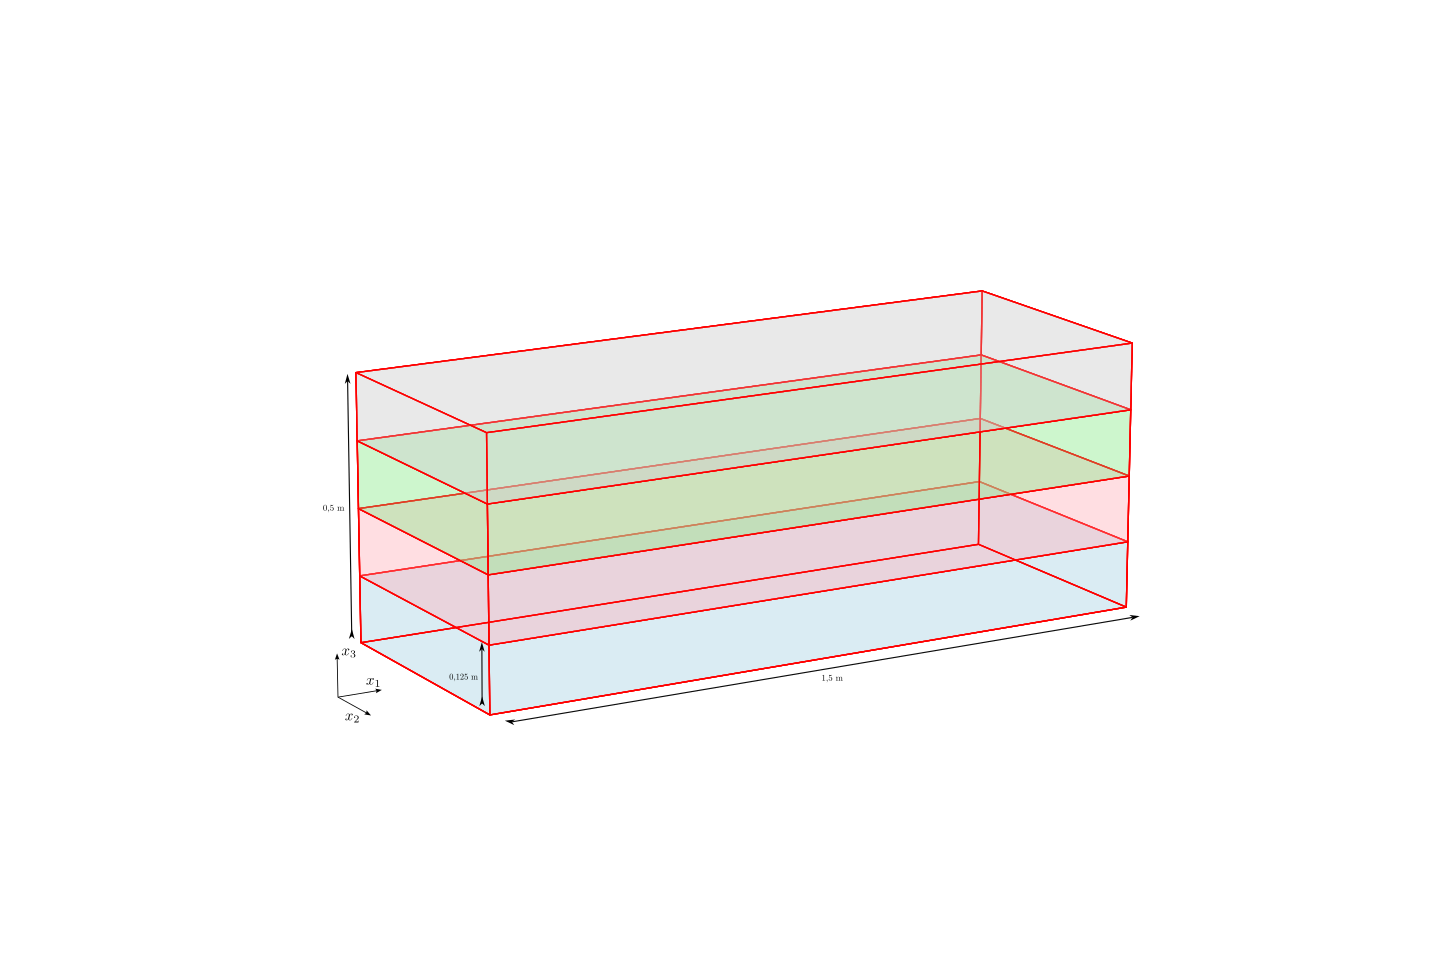
\includegraphics[width=.9\linewidth]{Img/Kapitola4/dif_dom.pdf}
            \caption{Sch\'{e}ma v\'{y}po\v{c}etn\'{\i} oblasti pro \'{u}lohu \ref{sub:Prob01}.}
            \label{fig:Probl01_domain}
        \end{figure}


        \begin{tcolorbox}[colframe=blue, title = \'{U}loha \ref{sub:Prob01}]
                            
            Parametry \'{u}lohy:
            \begin{itemize}
                \begin{multicols}{2}
                \item $\Omega = (0;1{,}0 \; \mathrm{m}) \times (0;0{,}5 \; \mathrm{m}) \times (0;0{,}5 \; \mathrm{m})$,
                \item $t \in \langle 0;0{,}1 \rangle \ \mathrm{s}$,
                \item $\nu = 1{,}552 \cdot 10^{-5} \ \mathrm{m^2 \ s^{-1}}$,
                \item $u_{in} = 2 \ \mathrm{m \ s^{-1}}$,
                \item $T_{ini} = 0 \ ^{\circ}\mathrm{C}$,
                \item $T_{in} = 25 \ ^{\circ}\mathrm{C}$,
                \item $D_{i} \in \{ 2{,}239 \cdot 10^{-i} \ | \ i \in \{ 1, 2, 3, 4\}\} \ \mathrm{m}^2 \ \mathrm{s}^{-1}$.
                \end{multicols}
            \end{itemize}
            
            Po\v{c}\'{a}te\v{c}n\'{\i} a okrajov\'{e} podm\'{\i}nky:
            \begin{itemize}
                \item V $\overline{\hat{\Omega}}$ nastav\'{\i}me po\v{c}\'{a}te\v{c}n\'{\i} podm\'{\i}nky dle sekc\'{\i} \ref{sec:NSEIniCon} a \ref{sec:ADEIniCon}.
                \item Na \v{c}\'{a}sti hranice $\hat{\Gamma}_{in}$ zvol\'{\i}me vstupn\'{\i} okrajov\'{e} podm\'{\i}nky popsan\'{e} v \ref{sec:NSEIniCon} a \ref{sec:ADEIniCon}.
                \item Pro $\hat{\Gamma}_{out}$ vol\'{\i}me odtokov\'{e} podm\'{\i}nky dle \ref{sec:NSEIniCon} a \ref{sec:ADEIniCon}.
                \item Na $\hat{\Gamma}_{w}$ pou\v{z}ijeme bounce-back okrajov\'{e} podm\'{\i}nky ze sekc\'{\i} \ref{sec:NSEIniCon} a \ref{sec:ADEIniCon}.
                \item Pro hranice mezi oblastmi p\v{r}edep\'{\i}\v{s}eme bounce-back okrajov\'{e} podm\'{\i}nky ze sekc\'{\i} \ref{sec:NSEIniCon} a \ref{sec:ADEIniCon}.
            \end{itemize}
            
            


            Parametry LBM:
            \begin{itemize}
                \item $N_x \times N_y \times N_z = (768 \times 384 \times 384)$,
                \item $\mathrm{Re} = 66 \ 666$,
                \item $\nu_{LBM} = 10^{-6}$, odpov\'{\i}d\'{a} $\Delta t \approx 10^{-7} s$.
            \end{itemize}

        \end{tcolorbox}

        \begin{figure}[H]
            \centering
            \includegraphics[width=\linewidth]{Img/Kapitola 3/Diffus_problem.png}
            \caption{Pr\r{u}\v{r}ez v\'{y}po\v{c}etn\'{\i} oblasti zn\'{a}zor\v{n}uj\'{\i}c\'{\i} \v{c}ty\v{r}i odd\v{e}len\'{e} \v{c}\'{a}sti oblasti s rozd\'{\i}ln\'{y}m difuzn\'{\i}m koeficientem $D_i$ pro $i \in \{1,2,3,4\}$ v \v{c}ase $t = 0{,}05 \ \mathrm{s}$. }
        \end{figure}
 


    \section{Testov\'{a}n\'{\i} p\v{r}estupov\'{e} okrajov\'{e} podm\'{\i}nky}
    \label{sec:TranConTest}

        V t\'{e}to sekci bude c\'{\i}lem otestovat implementovanou p\v{r}estupovovou okrajovou podm\'{\i}nku definovanou v sekci \ref{sec:TraBouCon}.
        
        Budeme uva\v{z}ovat 3D v\'{y}po\v{c}etn\'{\i} oblast ve tvaru kv\'{a}dru $\Omega = (0;1{,}5 \ \mathrm{m}) \times (0;0{,}5 \ \mathrm{m}) \times (0;0{,}5 \ \mathrm{m})$. Do n\'{\i} bude pevn\v{e} um\'{\i}st\v{e}no kv\'{a}drov\'{e} t\v{e}leso $\Omega_b$ o rozm\v{e}rech $(0{,}0252 \ \mathrm{m} \times 0{,}245 \ \mathrm{m} \times 0{,}105 \ \mathrm{m})$ s po\v{c}\'{a}te\v{c}n\'{\i} teplotou $T_{ini,b}$, viz obr\'{a}zek \ref{fig:Probl02_domain}. 
        
        P\v{r}i simulac\'{i}ch budeme uva\v{z}ovat r\r{u}zn\'{e} hodnoty jak pro koeficient p\v{r}estupu $\omega$, tak i pro velikost vstupn\'{\i} rychlosti $u_{in}$. D\'{a}le uva\v{z}ujeme i r\r{u}zn\'{e} prostorov\'{e} kroky $h$. P\v{r}edm\v{e}tem z\'{a}jmu pro n\'{a}s bude pr\r{u}m\v{e}rn\'{a} teplota na t\v{e}lese $\Omega_b$.

        \begin{figure}[H]
            \centering
            \includegraphics[width=\linewidth]{Img/Kapitola 3/Radiator_domain_without_mono.pdf}
            \caption{Sch\'{e}ma v\'{y}po\v{c}etn\'{\i} oblasti pro \'{u}lohu \ref{sub:Prob02}.}
            \label{fig:Probl02_domain}
        \end{figure}

        % C\'{\i}lem t\'{e}to sekce je ov\v{e}\v{r}it spr\'{a}vnost implementace v\'{y}po\v{c}tu s\'{\i}ly metodou v\'{y}m\v{e}ny hybnosti popsan\'{e} v sekci \ref{sec:MomExcMet}. Jeden z p\v{r}\'{\i}stup\r{u}, jak zjistit spr\'{a}vnost na\v{s}eho modelu, je pomoc\'{\i} bezrozm\v{e}rn\'{y}ch veli\v{c}in. V~na\v{s}em p\v{r}\'{\i}pad\v{e} se zam\v{e}\v{r}\'{\i}me na odporov\'{y} a vztlakov\'{y} koeficient.
        
        
        % Implementaci v\'{y}po\v{c}tu s\'{\i}ly ov\v{e}\v{r}\'{\i}me v\'{y}po\v{c}tem odporov\'{e}ho a vztlakov\'{e}ho koeficientu pomoc\'{\i} vztah\r{u} \eqref{eq:DraCoe} a \eqref{eq:LifCoe} aplikovan\'{y}ch na v\'{a}lec o polom\v{e}ru $r = 0{,}05 \ \mathrm{m}$, tj.
        
        % \begin{subequations}
        % \label{eq:NumCoe}
        % \begin{align}
        %     c_D = \frac{2F_1}{\rho U^{2}_{\infty}S}, \label{eq:NumDraCoe} \\
        %     c_L = \frac{2F_2}{\rho {U}^{2}_{\infty}S}, \label{eq:NumLifCoe}
        % \end{align}
        % \end{subequations}
        % kde $F_1,F_2$ jsou slo\v{z}ky vektoru s\'{\i}ly a $S = 0{,}1 \ \mathrm{m^2}$ odpov\'{\i}d\'{a} obsahu podstavy t\v{e}lesa dle \cite{schafer1996benchmark}. Na vstupu budeme p\v{r}edepisovat podm\'{\i}nky $P$ a $G$ definovan\'{e} v sekci \ref{sub:InfCon} a rychlost s parabolick\'{y}m profilem danou vztahem \eqref{eq:DefCasConInl2}. Dle maxim\'{a}ln\'{\i} p\v{r}edepisovan\'{e} rychlosti rozd\v{e}l\'{\i}me tuto \'{u}lohu na dv\v{e} pod\'{u}lohy: stabiln\'{\i} (s $U_{\infty} = 0{,}3 \ \mathrm{ m \; s^{-1}}$) a nestabiln\'{\i} (s $U_{\infty} = 1{,}5 \ \mathrm{ m \; s^{-1}}$).
        
        % \begin{figure}[H]
        %     \centering
        %     \includegraphics{Img/Kapitola 3/STurek3-1.pdf}
        %     \caption{Sch\'{e}ma um\'{\i}st\v{e}n\'{\i} kruhov\'{e}ho t\v{e}lesa o polom\v{e}ru podstavy $r = 0{,}05 \ \mathrm{m}$ ve 2D v\'{y}po\v{c}etn\'{\i} oblasti $\Omega = (0;1{,}64 \; \mathrm{m}) \times (0;0{,}41 \; \mathrm{m})$.}
        %     \label{fig:DomainST}
        % \end{figure}
        
        \subsection{P\v{r}estupov\'{a} OP}
        \label{sub:Prob02}
        
    
        \begin{tcolorbox}[colframe=blue, title = \'{U}loha \ref{sub:Prob02}]
                            
            Parametry \'{u}lohy:
            \begin{itemize}
                \begin{multicols}{2}
                \item $\Omega = (0;1{,}5 \; \mathrm{m}) \times (0;0{,}5 \; \mathrm{m}) \times (0;0{,}5 \; \mathrm{m})$,
                \item $t \in \langle 0;0{,}1 \rangle \ \mathrm{s}$,
                \item $\nu = 1{,}552 \cdot 10^{-5} \ \mathrm{m^2 \ s^{-1}}$,
                \item $u_{in} \in \{ 1, 4, 8, 12, 16, 20 \} \ \mathrm{m \ s^{-1}}$, 
                \item $T_{ini,a} = 25 \ ^{\circ}\mathrm{C}$,
                \item $T_{in} = 25 \ ^{\circ}\mathrm{C}$,
                \item $T_{ini,b} = 75 \ ^{\circ}\mathrm{C}$,
                \item $D_{a} = 2{,}239 \cdot 10^{-5} \ \mathrm{m^2 \ s^{-1}}$, 
                \item $D_b = 9{,}700 \cdot 10^{-5} \ \mathrm{m^2 \ s^{-1}}$,
                \item $\omega = 0{,}05j$ \quad $\forall j \in \{ 1,2,\dots,20 \} \ \mathrm{kg \ s^{-3} \ K^{-1}}$.
                \end{multicols}
            \end{itemize}
            
            Po\v{c}\'{a}te\v{c}n\'{\i} a okrajov\'{e} podm\'{\i}nky:
            \begin{itemize}
                \item V $\overline{\hat{\Omega}}$ nastav\'{\i}me po\v{c}\'{a}te\v{c}n\'{\i} podm\'{\i}nky dle sekc\'{\i} \ref{sec:NSEIniCon} a \ref{sec:ADEIniCon}.
                \item Na \v{c}\'{a}sti hranice $\hat{\Gamma}_{in}$ zvol\'{\i}me vstupn\'{\i} okrajov\'{e} podm\'{\i}nky popsan\'{e} v \ref{sec:NSEIniCon} a \ref{sec:ADEIniCon}.
                \item Pro $\hat{\Gamma}_{out}$ vol\'{\i}me odtokov\'{e} podm\'{\i}nky dle \ref{sec:NSEIniCon} a \ref{sec:ADEIniCon}.
                \item Na $\hat{\Gamma}_{w}$ pou\v{z}ijeme bounce-back okrajov\'{e} podm\'{\i}nky ze sekc\'{\i} \ref{sec:NSEIniCon} a \ref{sec:ADEIniCon}.
                \item Pro t\v{e}leso $\overline{\hat{\Omega}}_b$ vol\'{\i}me n\'{a}sleduj\'{\i}c\'{\i} okrajov\'{e} podm\'{\i}nky: \begin{itemize}
                    \item Pro NSR sch\'{e}ma vol\'{\i}me na $\overline{\hat{\Omega}}_b$ bounce-back okrajovou podm\'{\i}nku dle \ref{sec:NSEIniCon},
                    \item V ADR sch\'{e}matu pou\v{z}ijeme na $\hat{\Gamma}_b$ p\v{r}estupovou podm\'{\i}nku, viz \ref{sec:ADEIniCon}.  
                \end{itemize}
            \end{itemize}
            
            Parametry LBM:
            \begin{itemize}
                \item $N_x \times N_y \times N_z \in \{ 96i \times 32i \times 32i\ | \ i \in \{ 3,4,\dots,8 \} \} $,
                \item $\mathrm{Re} \in \langle 33 \ 333, 666 \ 666 \rangle$,
                \item $\nu_{LBM} = 10^{-6}$, odpov\'{\i}d\'{a} $\Delta t \approx 10^{-7} s$.
            \end{itemize}

        \end{tcolorbox}
        
        
        \begin{figure}[H]
            \centering
            \includegraphics[width=.95\linewidth, clip, trim=1.45cm 0.95cm 2cm 1.7cm]{Img/Kapitola 3/Problem02_all_transfers.pdf}
            \caption{Graf z\'{a}vislosti pr\r{u}m\v{e}rn\'{e} teploty na t\v{e}lese $\Omega_b$ na \v{c}ase $t$ pro \'{u}lohu \ref{sub:Prob02} a pro r\r{u}zn\'{e} hodnoty koeficientu p\v{r}estupu $\omega$, prostorov\'{y} krok $h = 1{,}969\cdot 10^{-3} \ \mathrm{m}$ odpov\'{\i}daj\'{\i}c\'{\i} m\v{r}\'{\i}\v{z}ce (768, 256, 256), \v{c}asov\'{y} krok $\Delta t =  2{,}497 \cdot 10^{-7}$ s a velikost vstupn\'{\i} rychlosti $u_{in} = 1 \ \mathrm{m \ s^{-1}}$. }
            \label{fig:Prob05_diff_h}
        \end{figure}

        \begin{figure}[H]
            \centering
            \includegraphics[width=\linewidth, trim=4cm 4cm 4cm 8cm]{Img/Kapitola 3/Probl10_a.pdf}
            \caption{Grafy zobrazuj\'{\i}c\'{\i} z\'{a}vislost pr\r{u}m\v{e}rn\'{e} teploty $T$ na \v{c}ase $t$ pro \'{u}lohu \ref{sub:Prob02} a pro r\r{u}zn\'{e} velikosti vstupn\'{\i} rychlosti $u_{in}$. Vyobrazeny jsou grafy pro r\r{u}zn\'{e} volby koeficientu p\v{r}estupu $\omega$. Ve v\v{s}ech grafech uva\v{z}ujeme prostorov\'{y} krok $h = 1{,}969 \cdot 10^{-3} \ \mathrm{m}$ odpov\'{\i}daj\'{\i}c\'{\i} m\v{r}\'{\i}\v{z}ce (768, 256, 256) a \v{c}asov\'{y} krok $\Delta t = 1{,}015 \cdot 10^{-7} \ \mathrm{s}$.}
            \label{fig:Probl10_a}
        \end{figure}

        \begin{figure}[H]
            \centering
            \includegraphics[width=\linewidth, trim=4cm 4cm 4cm 8cm]{Img/Kapitola 3/Probl10_b.pdf}
            \caption{Grafy zobrazuj\'{\i}c\'{\i} z\'{a}vislost pr\r{u}m\v{e}rn\'{e} teploty $T$ na \v{c}ase $t$ pro \'{u}lohu \ref{sub:Prob02} a pro r\r{u}zn\'{e} hodnoty koeficientu p\v{r}estupu $\omega$. Vyobrazeny jsou grafy pro r\r{u}zn\'{e} hodnoty vstupn\'{\i} rychlosti $u_{in}$. Ve v\v{s}ech grafech uva\v{z}ujeme prostorov\'{y} krok $h = 1{,}969 \cdot 10^{-3} \ \mathrm{m}$ odpov\'{\i}daj\'{\i}c\'{\i} m\v{r}\'{\i}\v{z}ce (768, 256, 256) a \v{c}asov\'{y} krok $\Delta t = 1{,}015 \cdot 10^{-7} \ \mathrm{s}$.}
            \label{fig:Probl10_b}
        \end{figure}





        \subsection{V\'{y}sledky \'{u}lohy \ref{sub:Prob02}}

            \'{U}loha \ref{sub:Prob02} simuluje nastaven\'{\i} p\v{r}estupov\'{e} okrajov\'{e} podm\'{\i}nky v modelu. P\v{r}edm\v{e}tem zkoum\'{a}n\'{\i} zde je v\'{y}voj pr\r{u}m\v{e}rn\'{e} teploty $T_{mean}$ v \v{c}ase $t$. Na grafu \ref{fig:Prob05_diff_h} pozorujeme z\'{a}vislost pr\r{u}m\v{e}rn\'{e} teploty pro r\r{u}zn\'{e} koeficienty p\v{r}estupu $\omega$ a vstupn\'{\i} rychlost $u_{in} = 1 \ \mathrm{m \ s^{-1}}$. Z grafu je z\v{r}ejm\'{e}, \v{z}e se zvy\v{s}uj\'{\i}c\'{\i} se hodnotou $\omega$ se \'{u}\v{c}innost chlazen\'{\i} zvy\v{s}uje a\v{z} do ur\v{c}it\'{e}ho limitn\'{\i}ho stavu. Na obr\'{a}zku \ref{fig:Probl10_b} je tato situace vyobrazena pro r\r{u}zn\'{e} hodnoty po\v{c}\'{a}te\v{c}n\'{\i} rychlosti $u_{in}$ a pro vybran\'{e} koeficienty p\v{r}estupu $\omega$. Lze nahl\'{e}dnout, \v{z}e i pro vy\v{s}\v{s}\'{\i} hodnoty vstupn\'{\i} rychlosti pr\r{u}m\v{e}rn\'{e} teploty konverguj\'{\i}.
        
            Z obr\'{a}zku \ref{fig:Probl10_a} lze vy\v{c}\'{\i}st, \v{z}e pro mal\'{e} koeficienty p\v{r}estupu t\'{e}m\v{e}\v{r} nez\'{a}vis\'{\i} na velikosti vstupn\'{\i} rychlosti. Pro hodnoty $\omega$ bl\'{\i}zk\'{e} 1 jsou ji\v{z} rozd\'{\i}ly mezi pr\r{u}m\v{e}rn\'{y}mi teplotami nezanedbateln\'{e}, ale i p\v{r}esto tyto rozd\'{\i}ly nejsou tak markantn\'{\i} v porovn\'{a}n\'{\i} s rychlostmi na vstupu. 
        

        \subsection{Pozn\'{a}mka k implementaci p\v{r}estupov\'{e} okrajov\'{e} podm\'{\i}nky}

            P\v{r}i implementaci p\v{r}estupov\'{e} okrajov\'{e} podm\'{\i}nky do\v{s}lo k odhalen\'{\i} chyby, kv\r{u}li kter\'{e} teplota unikala do okol\'{\i} i p\v{r}i nulov\'{e}m koeficientu p\v{r}estupu. Po lokalizaci chyby bylo zji\v{s}teno, \v{z}e probl\'{e}m nast\'{a}v\'{a} v situaci, kdy dojde ke kontaktu st\v{e}n oblasti s p\v{r}ek\'{a}\v{z}kou, tj. $\exists k \in \{0,1,2,\dots,6\}$ takov\'{e}, \v{z}e
            \begin{equation}
                g(\boldsymbol{x}_b + \xi_k \Delta t, t) = g(\boldsymbol{x}_w, t), 
            \end{equation}
            pro n\v{e}jak\'{e} uzly $\boldsymbol{x}_b$ a $\boldsymbol{x}_w$ ozna\v{c}uj\'{\i}c\'{\i} po \v{r}ad\v{e} uzel t\v{e}lesa a uzel st\v{e}ny. 
        
            Pro vy\v{r}e\v{s}en\'{\i} t\'{e}to chyby se nakonec uk\'{a}zalo nutn\'{e} do p\v{r}estupov\'{e} podm\'{\i}nky zahrnout je\v{s}t\v{e} i tento p\v{r}\'{\i}pad, tedy situaci, kdy se uzly t\v{e}lesa nach\'{a}z\'{\i} v kontaktu s uzlem zdi.


        

    % \section{Hled\'{a}n\'{\i} optim\'{a}ln\'{\i}ho rozm\v{e}ru radi\'{a}toru}
    % \label{sec:OptRad}
    
    %     Tato sekce se bude v\v{e}novat hled\'{a}n\'{\i} optim\'{a}ln\'{\i}ho tvaru radi\'{a}toru pro v\r{u}z studentsk\'{e} elektrick\'{e} formule FSE.12. Jak ji\v{z} bylo zm\'{\i}n\v{e}no, chlad\'{\i}c\'{\i} syst\'{e}m se nach\'{a}z\'{\i} v zadn\'{\i} \v{c}\'{a}sti vozu, proto p\v{r}i modelov\'{a}n\'{\i} v\'{y}po\v{c}etn\'{\i} oblasti lze \v{c}\'{a}ste\v{c}n\v{e} zanedbat geometrii p\v{r}edn\'{\i} \v{c}\'{a}sti vozu.

    %     Budeme uva\v{z}ovat op\v{e}t 3D v\'{y}po\v{c}etn\'{\i} oblast ve tvaru kv\'{a}dru $\Omega = (0;1{,}5 \ \mathrm{m}) \times (0;0{,}5 \ \mathrm{m}) \times (0;0{,}5 \ \mathrm{m})$, do kter\'{e} budou vlo\v{z}eny 2 t\v{e}lesa. Prvn\'{\i} z nich p\v{r}edstavuje \v{c}\'{a}st monokoku formule $\Omega_m$, kter\'{y} je um\'{\i}st\v{e}n jako na obr\'{a}zku \ref{fig:Probl06_domain}. Toto t\v{e}leso se bude v p\v{r}\'{\i}pad\v{e} \v{r}e\v{s}en\'{\i} NSR i ADR chovat jako pevn\'{a} p\v{r}ek\'{a}\v{z}ka, od kter\'{e} se vzduch i teplota odr\'{a}\v{z}\'{\i}. Druh\'{e} t\v{e}leso $\Omega_r$ p\v{r}edstavuje primitivn\'{\i} chladi\v{c}, u kter\'{e}ho prozat\'{\i}m zanedb\'{a}v\'{a}me geometrii vo\v{s}tiny, tud\'{\i}\v{z} v modelu je vyobrazen jako kv\'{a}dr. Chladi\v{c} se bude pro sch\'{e}ma NSR chovat jako pevn\'{a} p\v{r}ek\'{a}\v{z}ka, p\v{r}i \v{r}e\v{s}en\'{\i} ADR sch\'{e}matu budeme uva\v{z}ovat po\v{c}\'{a}te\v{c}n\'{\i} teplotu chladi\v{c}e $T_{ini,b}$. P\v{r}edpokl\'{a}dejme, \v{z}e radi\'{a}tor je vyroben z hlin\'{\i}ku. 
        
    %     % Po\v{z}adovan\'{a} plocha chladi\v{c}e kolm\'{a} na osu $x$ byla stanovena na $S\approx 25 000 \ \mathrm{mm^2}$. Navrhnut\'{e} a testovan\'{e} rozm\v{e}ry chladi\v{c}e byly zvoleny dle platn\'{y}ch pravidel a mo\v{z}nost\'{\i} v\'{y}robce.

    %     C\'{\i}lem t\'{e}to \'{u}lohy bude porovnat v\'{y}sledky pr\r{u}m\v{e}n\'{y}ch teplot $T_{mean}$ na chladi\v{c}\'{\i}ch a tak rozhodnout, jak\'{e} rozm\v{e}ry chladi\v{c}e jsou optim\'{a}ln\'{\i} pro takto zvolenou \'{u}lohu.
            
    %     \begin{figure}[H]
    %         \centering
    %         \includegraphics[width=\linewidth]{Img/Kapitola 3/Radiator_domain_with_mono.pdf}
    %         \caption{Sch\'{e}ma v\'{y}po\v{c}etn\'{\i} oblasti pro \'{u}lohu \ref{sub:Prob06}, kde \v{s}\'{\i}\v{r}ka $w$ a v\'{y}\v{s}ka $\ell$ v\'{y}m\v{e}n\'{\i}ku jsou parametry \'{u}lohy.}
    %         \label{fig:Probl06_domain}
    %     \end{figure}
        

    %     \subsection{Hled\'{a}n\'{\i} optim\'{a}ln\'{\i}ho chladi\v{c}e}
    %     \label{sub:Prob06}
        
    %         \begin{tcolorbox}[colframe=blue, title = \'{U}loha \ref{sub:Prob06}]
                                
    %             Parametry \'{u}lohy:
    %             \begin{itemize}
    %                 \begin{multicols}{2}
    %                 \item $\Omega = (0;1{,}5 \; \mathrm{m}) \times (0;0{,}5 \; \mathrm{m}) \times (0;0{,}5 \; \mathrm{m})$,
    %                 \item $t \in \langle 0;0{,}1 \rangle \ \mathrm{s}$,
    %                 \item $\nu = 1{,}552 \cdot 10^{-5} \ \mathrm{m^2 \ s^{-1}}$,
    %                 \item $u_{in} = 16 \ \mathrm{m \ s^{-1}}$, 
    %                 \item $T_{ini,a} = 25 \ ^{\circ}\mathrm{C}$,
    %                 \item $T_{in} = 25 \ ^{\circ}\mathrm{C}$,
    %                 \item $T_{ini,b} = 75 \ ^{\circ}\mathrm{C}$,
    %                 \item $D_{a} = 2{,}239 \cdot 10^{-5} \ \mathrm{m^2 \ s^{-1}}$, 
    %                 \item $D_b = 9{,}700 \cdot 10^{-5} \ \mathrm{m^2 \ s^{-1}}$,
    %                 \item $\omega = 1 \ \mathrm{kg \ s^{-3} \ K^{-1}}$.
    %                 \end{multicols}
    %                 \item ($w$,$\ell$) $\in \{ (250;100), (245;100), (245;105), (240;105), (235,105), (235,110), (230,110), \\ (225,110), (225,115), (220,110), (220,115), (215,115), (215,120), (210, 120), (210,115), \\ (205,120), (205,125), (200,125), (200,120), (200,130), (195,125), (195,130), (190,130), \\(190,135), (185,135) \} \ \mathrm{mm}$ 
    %             \end{itemize}
                
    %             Po\v{c}\'{a}te\v{c}n\'{\i} a okrajov\'{e} podm\'{\i}nky:
    %             \begin{itemize}
    %                 \item V $\overline{\hat{\Omega}}$ nastav\'{\i}me po\v{c}\'{a}te\v{c}n\'{\i} podm\'{\i}nky dle sekc\'{\i} \ref{sec:NSEIniCon} a \ref{sec:ADEIniCon}.
    %                 \item Na \v{c}\'{a}sti hranice $\hat{\Gamma}_{in}$ zvol\'{\i}me vstupn\'{\i} okrajov\'{e} podm\'{\i}nky popsan\'{e} v \ref{sec:NSEIniCon} a \ref{sec:ADEIniCon}.
    %                 \item Pro $\hat{\Gamma}_{out}$ vol\'{\i}me odtokov\'{e} podm\'{\i}nky dle \ref{sec:NSEIniCon} a \ref{sec:ADEIniCon}.
    %                 \item Na $\hat{\Gamma}_{w}$ pou\v{z}ijeme bounce-back okrajov\'{e} podm\'{\i}nky ze sekc\'{\i} \ref{sec:NSEIniCon} a \ref{sec:ADEIniCon}.
    %                 \item Pro t\v{e}leso $\overline{\hat{\Omega}}_b$ vol\'{\i}me n\'{a}sleduj\'{\i}c\'{\i} okrajov\'{e} podm\'{\i}nky: \begin{itemize}
    %                     \item Pro NSR sch\'{e}ma vol\'{\i}me na $\overline{\hat{\Omega}}_b$ bounce-back okrajovou podm\'{\i}nku dle \ref{sec:NSEIniCon},
    %                     \item V ADR sch\'{e}matu pou\v{z}ijeme na $\hat{\Gamma}_b$ p\v{r}estupovou podm\'{\i}nku, viz \ref{sec:ADEIniCon}.  
    %                 \end{itemize}
    %             \end{itemize}
                
    %             Parametry LBM:
    %             \begin{itemize}
    %                 \item $N_x \times N_y \times N_z \in \{ 96i \times 32i \times 32i\ | \ i \in \{ 3,4,\dots,8 \} \} $,
    %                 \item $\mathrm{Re} \approx 533 \ 333$,
    %                 \item $\nu_{LBM} = 10^{-6}$, odpov\'{\i}d\'{a} $\Delta t \approx 10^{-7} s$.
    %             \end{itemize}

    %         \end{tcolorbox}

    %         \begin{figure}[H]
    %             \centering
    %             \includegraphics[width=.9\linewidth, clip, trim=3cm 0.65cm 3.5cm 2cm]{Img/Kapitola 3/Probl06_all_rads.pdf}
    %         \end{figure}
    %         \begin{figure}[H]
    %             \centering
    %             \includegraphics[width=.9\linewidth, clip, trim=2.5cm 0.65cm 3.5cm 2cm]{Img/Kapitola 3/Probl06_all_rads_zoom.pdf}
    %             \caption{Grafy z\'{a}vislosti pr\r{u}m\v{e}rn\'{e} teploty $T_{mean}$ na t\v{e}lese $\Omega_b$ na \v{c}ase $t$ pro \'{u}lohu \ref{sub:Prob06} a pro vybran\'{e} rozm\v{e}ry radi\'{a}toru, prostorov\'{y} krok $h = 1{,}969\cdot 10^{-3} \ \mathrm{m}$ odpov\'{\i}daj\'{\i}c\'{\i} m\v{r}\'{\i}\v{z}ce (768, 256, 256) a \v{c}asov\'{y} krok $\Delta t =  2{,}497 \cdot 10^{-7}$ s. Prvn\'{\i} graf zn\'{a}zor\v{n}uje cel\'{y} \v{c}asov\'{y} pr\r{u}b\v{e}h, ve druh\'{e}m je pro detail p\v{r}ibl\'{\i}\v{z}en fin\'{a}ln\'{\i} \v{c}asov\'{y} \'{u}sek.}
    %             \label{fig:Prob06_rads_all}
    %             \end{figure}

    %     \subsection{V\'{y}sledky \'{u}lohy \ref{sub:Prob06}}

    %         \'{U}loha \ref{sub:Prob06} simuluje nastaven\'{\i} modelu pro r\r{u}zn\'{e} geometrie radi\'{a}toru. P\v{r}edm\v{e}tem zkoum\'{a}n\'{\i} je zde z\'{a}vislost pr\r{u}m\v{e}rn\'{e} teploty radi\'{a}toru $T_{mean}$ na \v{c}ase $t$. Na grafech \ref{fig:Prob06_rads_all} je pro p\v{r}ehlednost vyobrazeno jen n\v{e}kolik r\r{u}zn\'{y}ch velikost\'{\i} radi\'{a}toru. Z graf\r{u} je patrn\'{e}, \v{z}e pro danou \'{u}lohu jsou v\'{y}sledn\'{e} hodnoty pr\r{u}m\v{e}rn\'{e} teploty v intervalu $\langle 39{,}53 ; 39{,}89 \rangle$ \textdegree C. Minim\'{a}ln\'{\i} hodnoty pr\r{u}m\v{e}rn\'{e} teploty je dosa\v{z}eno v p\v{r}\'{\i}pad\v{e} rozm\v{e}r\r{u} chladi\v{c}e $(210,115,25{,}2)$ mm.  

    %     \subsection{Pozn\'{a}mky k hled\'{a}n\'{\i} optim\'{a}ln\'{\i}ho chladi\v{c}e}

    %         V r\'{a}mci t\'{e}to \v{c}\'{a}sti byl hled\'{a}n optim\'{a}ln\'{\i} chladi\v{c}. Model chladi\v{c}e pou\v{z}it\'{y} v t\'{e}to pr\'{a}ci, jak ji\v{z} bylo zm\'{\i}n\v{e}no, neuva\v{z}uje vo\v{s}tinu radi\'{a}toru, a to z d\r{u}vodu vysok\'{y}ch n\'{a}rok\r{u} na rozli\v{s}en\'{\i}. Proto se jedn\'{a} o p\v{r}edb\v{e}\v{z}n\'{y} v\'{y}sledek, kter\'{y} je zat\'{\i}\v{z}en velkou chybou v porovn\'{a}n\'{\i} se skute\v{c}nou situac\'{\i}. B\v{e}hem pokra\v{c}uj\'{\i}c\'{\i}ho v\'{y}zkumu je v pl\'{a}nu zahrnout pokro\v{c}ilej\v{s}\'{\i} geometrii chladi\v{c}e, d\'{\i}ky \v{c}emu\v{z} bude simulace mnohem bl\'{\i}\v{z}e skute\v{c}nosti. 

    \section{Testov\'{a}n\'{\i} konvergence p\v{r}estupov\'{e} okrajov\'{e} podm\'{\i}nky}
        
        V t\'{e}to sekci budeme zkoumat chov\'{a}n\'{\i} teploty v oblasti okolo p\v{r}ek\'{a}\v{z}ky p\v{r}i pou\v{z}it\'{\i} p\v{r}estupov\'{e} okrajov\'{e} podm\'{\i}nky popsan\'{e} v sekci \ref{sec:TraBouCon}. V pr\r{u}b\v{e}hu v\'{y}zkumu byly pozorov\'{a}ny numerick\'{e} chyby v oblasti n\'{a}b\v{e}hov\'{e} hrany p\v{r}ek\'{a}\v{z}ky. 


        Pro optimalizaci v\'{y}po\v{c}tu pou\v{z}ijeme na st\v{e}nu $\Gamma_{top}$ symetrickou okrajovou podm\'{\i}nku, p\v{r}i v\'{y}po\v{c}tech u\v{s}et\v{r}\'{i}me polovinu pam\v{e}ti a budeme tak moci dos\'{a}hnout jemn\v{e}j\v{s}\'{i}ho rozli\v{s}en\'{i} s\'{i}t\v{e}. P\v{r}eci jen p\v{r}ipome\v{n}me, \v{z}e jsme p\v{r}i v\'{y}po\v{c}tech omezen\'{i} pam\v{e}t\'{i} grafick'{y}ch karet, kter\'{a} je st\'{a}le jednou z nejv\v{e}t\v{s}\'{i}ch p\v{r}ek\'{a}\v{z}ek p\v{r}i v\'{y}po\v{c}tu.



        V r\'{a}mci t\'{e}to sekce budeme ve v\'{y}po\v{c}tech sledovat chov\'{a}n\'{i} minim\'{a}ln\'{i} a maxim\'{a}ln\'{i} teploty v podoblasti $\overline{\hat{\Omega_{s}}}$ v\'{y}po\v{c}etn\'{\i} oblasti $\overline{\hat{\Omega}}$. 




   

        
        

        \subsection{P\v{r}estupov\'{a} OP pro $D_* \approx 10^{-3} \ \mathrm{m}^{2} \ \mathrm{s}^{-1}$}
        \label{sub:D10m3}
        
            \begin{tcolorbox}[colframe=blue, title = \'{U}loha \ref{sub:D10m3}]
                        
                Parametry \'{u}lohy:
                \begin{itemize}
                    \begin{multicols}{2}
                    \item $\Omega = (0;1{,}25 \; \mathrm{m}) \times (0;1 \; \mathrm{m}) \times (0;0{,}5 \; \mathrm{m})$,
                    \item $t \in \langle 0;10 \rangle \ \mathrm{s}$,
                    \item $\nu = 1{,}552 \cdot 10^{-5} \ \mathrm{m^2 \ s^{-1}}$,
                    \item $u_{in} = 1 \ \mathrm{m \ s^{-1}}$, 
                    \item $T_{ini,a} = 5 \ ^{\circ}\mathrm{C}$,
                    \item $T_{in} = 5 \ ^{\circ}\mathrm{C}$,
                    \item $T_{ini,b} = 5 \ ^{\circ}\mathrm{C}$,
                    \item $D_{a} = 2{,}239 \cdot 10^{-3} \ \mathrm{m^2 \ s^{-1}}$, 
                    \item $D_b = 9{,}700 \cdot 10^{-3} \ \mathrm{m^2 \ s^{-1}}$,
                    \item $\omega = 0{,}01 \  \mathrm{kg \ s^{-3} \ K^{-1}}$.
                    \end{multicols}
                \end{itemize}
                
                Po\v{c}\'{a}te\v{c}n\'{\i} a okrajov\'{e} podm\'{\i}nky:
                \begin{itemize}
                    \item V $\overline{\hat{\Omega}}$ nastav\'{\i}me po\v{c}\'{a}te\v{c}n\'{\i} podm\'{\i}nky dle sekc\'{\i} \ref{sec:NSEIniCon} a \ref{sec:ADEIniCon}.
                    \item Na \v{c}\'{a}sti hranice $\hat{\Gamma}_{in}$ zvol\'{\i}me vstupn\'{\i} okrajov\'{e} podm\'{\i}nky popsan\'{e} v \ref{sec:NSEIniCon} a \ref{sec:ADEIniCon}.
                    \item Pro $\hat{\Gamma}_{out}$ vol\'{\i}me odtokov\'{e} podm\'{\i}nky dle \ref{sec:NSEIniCon} a \ref{sec:ADEIniCon}.
                    \item Na $\hat{\Gamma}_{w}$ pou\v{z}ijeme bounce-back okrajov\'{e} podm\'{\i}nky ze sekc\'{\i} \ref{sec:NSEIniCon} a \ref{sec:ADEIniCon}.
                    \item Pro t\v{e}leso $\overline{\hat{\Omega}}_b$ vol\'{\i}me n\'{a}sleduj\'{\i}c\'{\i} okrajov\'{e} podm\'{\i}nky: \begin{itemize}
                        \item Pro NSR sch\'{e}ma vol\'{\i}me na $\overline{\hat{\Omega}}_b$ bounce-back okrajovou podm\'{\i}nku dle \ref{sec:NSEIniCon},
                        \item V ADR sch\'{e}matu pou\v{z}ijeme na $\hat{\Gamma}_b$ p\v{r}estupovou podm\'{\i}nku, viz \ref{sec:ADEIniCon}.  
                    \end{itemize}
                \end{itemize}
                
                Parametry LBM:
                \begin{itemize}
                    \item $N_x \times N_y \times N_z \in \{ 40i \times 32i \times 16i\ | \ i \in \{ 3,4,\dots,25 \} \} $,
                    \item $\mathrm{Re} = 33 \ 333$,
                    \item $\nu_{LBM} = 10^{-4}$, odpov\'{\i}d\'{a} $\Delta t \approx 10^{-5} s$.
                \end{itemize}
            \end{tcolorbox}

            \begin{table}[H]
                \centering
                % First subtable
                \begin{tabular}{p{0.25\textwidth}p{0.18\textwidth}p{0.18\textwidth}p{0.18\textwidth}}
                    \toprule
                    \multicolumn{4}{c}{\centering{$t=1.0 \ \mathrm{s}$}} \\ \midrule
                    Rozli\v{s}en\'{\i} s\'{\i}t\v{e} & \multicolumn{1}{p{2.5cm}}{Prostorov\'{y} krok $h \ [\mathrm{m}]$} & \multicolumn{1}{p{2.8cm}}{Minim\'{a}ln\'{\i} teplota $T_{min} \ [^\circ\mathrm{C}]$} & \multicolumn{1}{p{2.8cm}}{Minim\'{a}ln\'{\i} teplota $T_{min} \ [^\circ\mathrm{C}]$} \\ \midrule
                    $160 \times 128 \times 64$  & $7,81 \cdot  10^{-3}$ & 4,757 & 5,587 \\
                    $200 \times 160 \times 80$  & $6,25 \cdot  10^{-3}$ & 4,795 & 5,491 \\
                    $240 \times 192 \times 96$  & $5,21 \cdot  10^{-3}$ & 4,824 & 5,423 \\
                    $280 \times 224 \times 112$  & $4,46 \cdot  10^{-3}$ & 4,845 & 5,367 \\
                    $320 \times 256 \times 128$  & $3,91 \cdot  10^{-3}$ & 4,822 & 5,327 \\
                    $360 \times 288 \times 144$  & $3,47 \cdot  10^{-3}$ & 4,869 & 5,288 \\
                    $400 \times 320 \times 160$  & $3,13 \cdot  10^{-3}$ & 4,864 & 5,258 \\
                    $440 \times 352 \times 176$  & $2,84 \cdot  10^{-3}$ & 4,929 & 5,169 \\ 
                    \bottomrule

                \end{tabular}

                % Single caption for all subtables
                \caption{V\'{y}voj minim\'{a}ln\'{\i} a maxim\'{a}ln\'{\i} teploty v z\'{a}vislosti na rozli\v{s}en\'{\i} s\'{i}t\v{e} pro hodnotu difuzn\'{\i}ho koeficientu $D \approx 10^{-3}$ v \v{c}ase $t = 1 \ \mathrm{s}$.}
                \label{table:D10m3_1}
            \end{table}


            \begin{table}[H]
                \centering
                % First subtable
                \begin{tabular}{p{0.25\textwidth}p{0.18\textwidth}p{0.18\textwidth}p{0.18\textwidth}}
                    \toprule
                    \multicolumn{4}{c}{\centering{$t=3.0 \ \mathrm{s}$}} \\ \midrule
                    Rozli\v{s}en\'{\i} s\'{\i}t\v{e} & \multicolumn{1}{p{2.5cm}}{Prostorov\'{y} krok $h \ [\mathrm{m}]$} & \multicolumn{1}{p{2.8cm}}{Minim\'{a}ln\'{\i} teplota $T_{min} \ [^\circ\mathrm{C}]$} & \multicolumn{1}{p{2.8cm}}{Minim\'{a}ln\'{\i} teplota $T_{min} \ [^\circ\mathrm{C}]$} \\ \midrule
                    $160 \times 128 \times 64$  & $7,81 \cdot  10^{-3}$ & 4,771 & 5,593 \\
                    $200 \times 160 \times 80$  & $6,25 \cdot  10^{-3}$ & 4,802 & 5,494 \\
                    $240 \times 192 \times 96$  & $5,21 \cdot  10^{-3}$ & 4,828 & 5,424 \\
                    $280 \times 224 \times 112$  & $4,46 \cdot  10^{-3}$ & 4,847 & 5,367 \\
                    $320 \times 256 \times 128$  & $3,91 \cdot  10^{-3}$ & 4,865 & 5,322 \\
                    $360 \times 288 \times 144$  & $3,47 \cdot  10^{-3}$ & 4,879 & 5,287 \\
                    $400 \times 320 \times 160$  & $3,13 \cdot  10^{-3}$ & 4,888 & 5,258 \\
                    $440 \times 352 \times 176$  & $2,84 \cdot  10^{-3}$ & 4,931 & 5,169 \\ \bottomrule
                \end{tabular}
                % Single caption for all subtables
                \caption{V\'{y}voj minim\'{a}ln\'{\i} a maxim\'{a}ln\'{\i} teploty v z\'{a}vislosti na rozli\v{s}en\'{\i} s\'{i}t\v{e} pro hodnotu difuzn\'{\i}ho koeficientu $D \approx 10^{-3}$ v \v{c}ase $t = 3 \ \mathrm{s}$.}
                \label{table:D10m3_3}
            \end{table}

            \begin{table}[H]
                \centering
                % First subtable
                \begin{tabular}{p{0.25\textwidth}p{0.18\textwidth}p{0.18\textwidth}p{0.18\textwidth}}
                    \toprule
                    \multicolumn{4}{c}{\centering{$t=5.0 \ \mathrm{s}$}} \\ \midrule
                    Rozli\v{s}en\'{\i} s\'{\i}t\v{e} & \multicolumn{1}{p{2.5cm}}{Prostorov\'{y} krok $h \ [\mathrm{m}]$} & \multicolumn{1}{p{2.8cm}}{Minim\'{a}ln\'{\i} teplota $T_{min} \ [^\circ\mathrm{C}]$} & \multicolumn{1}{p{2.8cm}}{Minim\'{a}ln\'{\i} teplota $T_{min} \ [^\circ\mathrm{C}]$} \\ \midrule
                    $160 \times 128 \times 64$  & $7,81 \cdot  10^{-3}$ & 4,772 & 5,594 \\
                    $200 \times 160 \times 80$  & $6,25 \cdot  10^{-3}$ & 4,803 & 5,497 \\
                    $240 \times 192 \times 96$  & $5,21 \cdot  10^{-3}$ & 4,824 & 5,428 \\
                    $280 \times 224 \times 112$  & $4,46 \cdot  10^{-3}$ & 4,845 & 5,372 \\
                    $320 \times 256 \times 128$  & $3,91 \cdot  10^{-3}$ & 4,864 & 5,324 \\
                    $360 \times 288 \times 144$  & $3,47 \cdot  10^{-3}$ & 4,880 & 5,285 \\
                    $400 \times 320 \times 160$  & $3,13 \cdot  10^{-3}$ & 4,889 & 5,257 \\
                    $440 \times 352 \times 176$  & $2,84 \cdot  10^{-3}$ & 4,930 & 5,172 \\ \bottomrule
                \end{tabular}
                % Single caption for all subtables
                \caption{V\'{y}voj minim\'{a}ln\'{\i} a maxim\'{a}ln\'{\i} teploty v z\'{a}vislosti na rozli\v{s}en\'{\i} s\'{i}t\v{e} pro hodnotu difuzn\'{\i}ho koeficientu $D \approx 10^{-3}$ v \v{c}ase $t = 3 \ \mathrm{s}$.}
                \label{table:D10m3_5}
            \end{table}


            \begin{table}[H]
                \centering
                % First subtable
                \begin{tabular}{p{0.25\textwidth}p{0.18\textwidth}p{0.18\textwidth}p{0.18\textwidth}}
                    \toprule
                    \multicolumn{4}{c}{\centering{$t=10.0 \ \mathrm{s}$}} \\ \midrule
                    Rozli\v{s}en\'{\i} s\'{\i}t\v{e} & \multicolumn{1}{p{2.5cm}}{Prostorov\'{y} krok $h \ [\mathrm{m}]$} & \multicolumn{1}{p{2.8cm}}{Minim\'{a}ln\'{\i} teplota $T_{min} \ [^\circ\mathrm{C}]$} & \multicolumn{1}{p{2.8cm}}{Minim\'{a}ln\'{\i} teplota $T_{min} \ [^\circ\mathrm{C}]$} \\ \midrule
                    $160 \times 128 \times 64$  & $7,81 \cdot  10^{-3}$ & 4,772 & 5,596 \\
                    $200 \times 160 \times 80$  & $6,25 \cdot  10^{-3}$ & 4,802 & 5,497 \\
                    $240 \times 192 \times 96$  & $5,21 \cdot  10^{-3}$ & 4,826 & 5,427 \\
                    $280 \times 224 \times 112$  & $4,46 \cdot  10^{-3}$ & 4,847 & 5,368 \\
                    $320 \times 256 \times 128$  & $3,91 \cdot  10^{-3}$ & 4,863 & 5,325 \\
                    $360 \times 288 \times 144$  & $3,47 \cdot  10^{-3}$ & 4,878 & 5,289 \\
                    $400 \times 320 \times 160$  & $3,13 \cdot  10^{-3}$ & 4,889 & 5,257 \\
                    $440 \times 352 \times 176$  & $2,84 \cdot  10^{-3}$ & 4,932 & 5,168 \\ \bottomrule
                \end{tabular}
                % Single caption for all subtables
                \caption{V\'{y}voj minim\'{a}ln\'{\i} a maxim\'{a}ln\'{\i} teploty v z\'{a}vislosti na rozli\v{s}en\'{\i} s\'{i}t\v{e} pro hodnotu difuzn\'{\i}ho koeficientu $D \approx 10^{-3}$ v \v{c}ase $t = 3 \ \mathrm{s}$.}
                \label{table:D10m3_10}
            \end{table}



            \begin{figure}[h]
                \centering
                \includegraphics[width=\linewidth, trim=4cm 1cm 4cm 4cm]{Img/Kapitola4/d_10m3.pdf}
                \caption{Grafy zobrazuj\'{\i}c\'{\i} z\'{a}vislost minim\'{a}ln\'{\i} a maxim\'{a}ln\'{\i} teploty na prostorov\'{e}m kroku $h$ pro \'{u}lohu \ref{sub:D10m3} a pro r\r{u}zn\'{e} \v{c}asy $t$.}
                \label{fig:Prob10m3}
            \end{figure}


        \subsection{V\'{y}sledky \'{u}lohy \ref{sub:D10m3}}
    
            \'{U}loha \ref{sub:D10m3} simuluje nastaven\'{\i} p\v{r}estupov\'{e} okrajov\'{e} podm\'{\i}nky v modelu pro r\r{u}zn\'{e} hodnoty prostorov\'{e}ho kroku $h$. P\v{r}edm\v{e}tem zkoum\'{a}n\'{\i} je zde v\'{y}voj minim\'{a}ln\'{i} $T_{min}$ a maxim\'{a}ln\'{i} $T_{max}$ teploty v z\'{a}vislosti zmen\v{s}uj\'{i}c\'{i}m se prostorov\'{e}m kroku $h$. 
            

            % \'{U}loha \ref{sub:Prob02} simuluje nastaven\'{\i} p\v{r}estupov\'{e} okrajov\'{e} podm\'{\i}nky v modelu. P\v{r}edm\v{e}tem zkoum\'{a}n\'{\i} zde je v\'{y}voj pr\r{u}m\v{e}rn\'{e} teploty $T_{mean}$ v \v{c}ase $t$. Na grafu \ref{fig:Prob05_diff_h} pozorujeme z\'{a}vislost pr\r{u}m\v{e}rn\'{e} teploty pro r\r{u}zn\'{e} koeficienty p\v{r}estupu $\omega$ a vstupn\'{\i} rychlost $u_{in} = 1 \ \mathrm{m \ s^{-1}}$. Z grafu je z\v{r}ejm\'{e}, \v{z}e se zvy\v{s}uj\'{\i}c\'{\i} se hodnotou $\omega$ se \'{u}\v{c}innost chlazen\'{\i} zvy\v{s}uje a\v{z} do ur\v{c}it\'{e}ho limitn\'{\i}ho stavu. Na obr\'{a}zku \ref{fig:Probl10_b} je tato situace vyobrazena pro r\r{u}zn\'{e} hodnoty po\v{c}\'{a}te\v{c}n\'{\i} rychlosti $u_{in}$ a pro vybran\'{e} koeficienty p\v{r}estupu $\omega$. Lze nahl\'{e}dnout, \v{z}e i pro vy\v{s}\v{s}\'{\i} hodnoty vstupn\'{\i} rychlosti pr\r{u}m\v{e}rn\'{e} teploty konverguj\'{\i}.
        
            % Z obr\'{a}zku \ref{fig:Probl10_a} lze vy\v{c}\'{\i}st, \v{z}e pro mal\'{e} koeficienty p\v{r}estupu t\'{e}m\v{e}\v{r} nez\'{a}vis\'{\i} na velikosti vstupn\'{\i} rychlosti. Pro hodnoty $\omega$ bl\'{\i}zk\'{e} 1 jsou ji\v{z} rozd\'{\i}ly mezi pr\r{u}m\v{e}rn\'{y}mi teplotami nezanedbateln\'{e}, ale i p\v{r}esto tyto rozd\'{\i}ly nejsou tak markantn\'{\i} v porovn\'{a}n\'{\i} s rychlostmi na vstupu. 









            




        \subsection{P\v{r}estupov\'{a} OP pro $D_* \approx 10^{-5} \ \mathrm{m}^{2} \ \mathrm{s}^{-1}$}
        \label{sub:D10m5}
        
    
            \begin{tcolorbox}[colframe=blue, title = \'{U}loha \ref{sub:D10m5}]
                                    
                Parametry \'{u}lohy:
                \begin{itemize}
                    \begin{multicols}{2}
                    \item $\Omega = (0;1{,}25 \; \mathrm{m}) \times (0;1 \; \mathrm{m}) \times (0;0{,}5 \; \mathrm{m})$,
                    \item $t \in \langle 0;0{,}1 \rangle \ \mathrm{s}$,
                    \item $\nu = 1{,}552 \cdot 10^{-5} \ \mathrm{m^2 \ s^{-1}}$,
                    \item $u_{in} = 1 \ \mathrm{m \ s^{-1}}$, 
                    \item $T_{ini,a} = 5 \ ^{\circ}\mathrm{C}$,
                    \item $T_{in} = 5 \ ^{\circ}\mathrm{C}$,
                    \item $T_{ini,b} = 5 \ ^{\circ}\mathrm{C}$,
                    \item $D_{a} = 2{,}239 \cdot 10^{-3} \ \mathrm{m^2 \ s^{-1}}$, 
                    \item $D_b = 9{,}700 \cdot 10^{-3} \ \mathrm{m^2 \ s^{-1}}$,
                    \item $\omega = 0{,}01 \  \mathrm{kg \ s^{-3} \ K^{-1}}$.
                    \end{multicols}
                \end{itemize}
                
                Po\v{c}\'{a}te\v{c}n\'{\i} a okrajov\'{e} podm\'{\i}nky:
                \begin{itemize}
                    \item V $\overline{\hat{\Omega}}$ nastav\'{\i}me po\v{c}\'{a}te\v{c}n\'{\i} podm\'{\i}nky dle sekc\'{\i} \ref{sec:NSEIniCon} a \ref{sec:ADEIniCon}.
                    \item Na \v{c}\'{a}sti hranice $\hat{\Gamma}_{in}$ zvol\'{\i}me vstupn\'{\i} okrajov\'{e} podm\'{\i}nky popsan\'{e} v \ref{sec:NSEIniCon} a \ref{sec:ADEIniCon}.
                    \item Pro $\hat{\Gamma}_{out}$ vol\'{\i}me odtokov\'{e} podm\'{\i}nky dle \ref{sec:NSEIniCon} a \ref{sec:ADEIniCon}.
                    \item Na $\hat{\Gamma}_{w}$ pou\v{z}ijeme bounce-back okrajov\'{e} podm\'{\i}nky ze sekc\'{\i} \ref{sec:NSEIniCon} a \ref{sec:ADEIniCon}.
                    \item Pro t\v{e}leso $\overline{\hat{\Omega}}_b$ vol\'{\i}me n\'{a}sleduj\'{\i}c\'{\i} okrajov\'{e} podm\'{\i}nky: \begin{itemize}
                        \item Pro NSR sch\'{e}ma vol\'{\i}me na $\overline{\hat{\Omega}}_b$ bounce-back okrajovou podm\'{\i}nku dle \ref{sec:NSEIniCon},
                        \item V ADR sch\'{e}matu pou\v{z}ijeme na $\hat{\Gamma}_b$ p\v{r}estupovou podm\'{\i}nku, viz \ref{sec:ADEIniCon}.  
                    \end{itemize}
                \end{itemize}
                
                Parametry LBM:
                \begin{itemize}
                    \item $N_x \times N_y \times N_z \in \{ 40i \times 32i \times 16i\ | \ i \in \{ 3,4,\dots,25 \} \} $,
                    \item $\mathrm{Re} = 33 \ 333$,
                    \item $\nu_{LBM} = 10^{-4}$, odpov\'{\i}d\'{a} $\Delta t \approx 10^{-5} s$.
                \end{itemize}

            \end{tcolorbox}

    \section{Experiment CUBI}

        V t\'{e}to sekci se zam\v{e}\v{r}\'{i}me na simulaci prob\'{i}haj\'{i}c\'{i}ho experimentu ve v\'{y}zkumn\'{e}m centru SENSE, v americk\'{e}m ...
        
        Projekt zkoum\'{a} v\'{y}voj rychlostn\'{i}ho a teplotn\'{i}ho profilu v oblasti mezn\'{i} vrstv\v{e} okolo p\v{r}ek\'{a}\v{z}ky - tzv. CUBIho. Experiment prob\'{i}h\'{a} ve v\v{e}trn\'{e}m tunelu, jeho\v{z} pr\r{u}\v{r}ez je ve tvaru \v{c}terve o hran\v{e} $1 \ \mathrm{m}$.
        
        Uva\v{z}ujme tedy v\'{y}po\v{c}etn\'{\i} oblast $\overline{\hat{\Omega}}$. P\v{r}ek\'{a}\v{z}ku $\overline{\hat{\Omega}}_b$ v tomto p\v{r}\'{\i}pad\v{e} bude tvo\v{r}it t\v{e}leso slo\v{z}en\'{e} ze t\v{r}\'{\i} toto\v{z}n\'{y}ch krychl\'{\i} o hran\v{e} $0.125 \ \mathrm{m}$ sestaven\'{y}ch do tvaru p\'{i}smene L, viz. obr\'{a}zek \ref{fig:CUBI}. Toto t\v{e}leso dostalo jm\'{e}no CUBI.

        \begin{figure}[H]
            \centering
            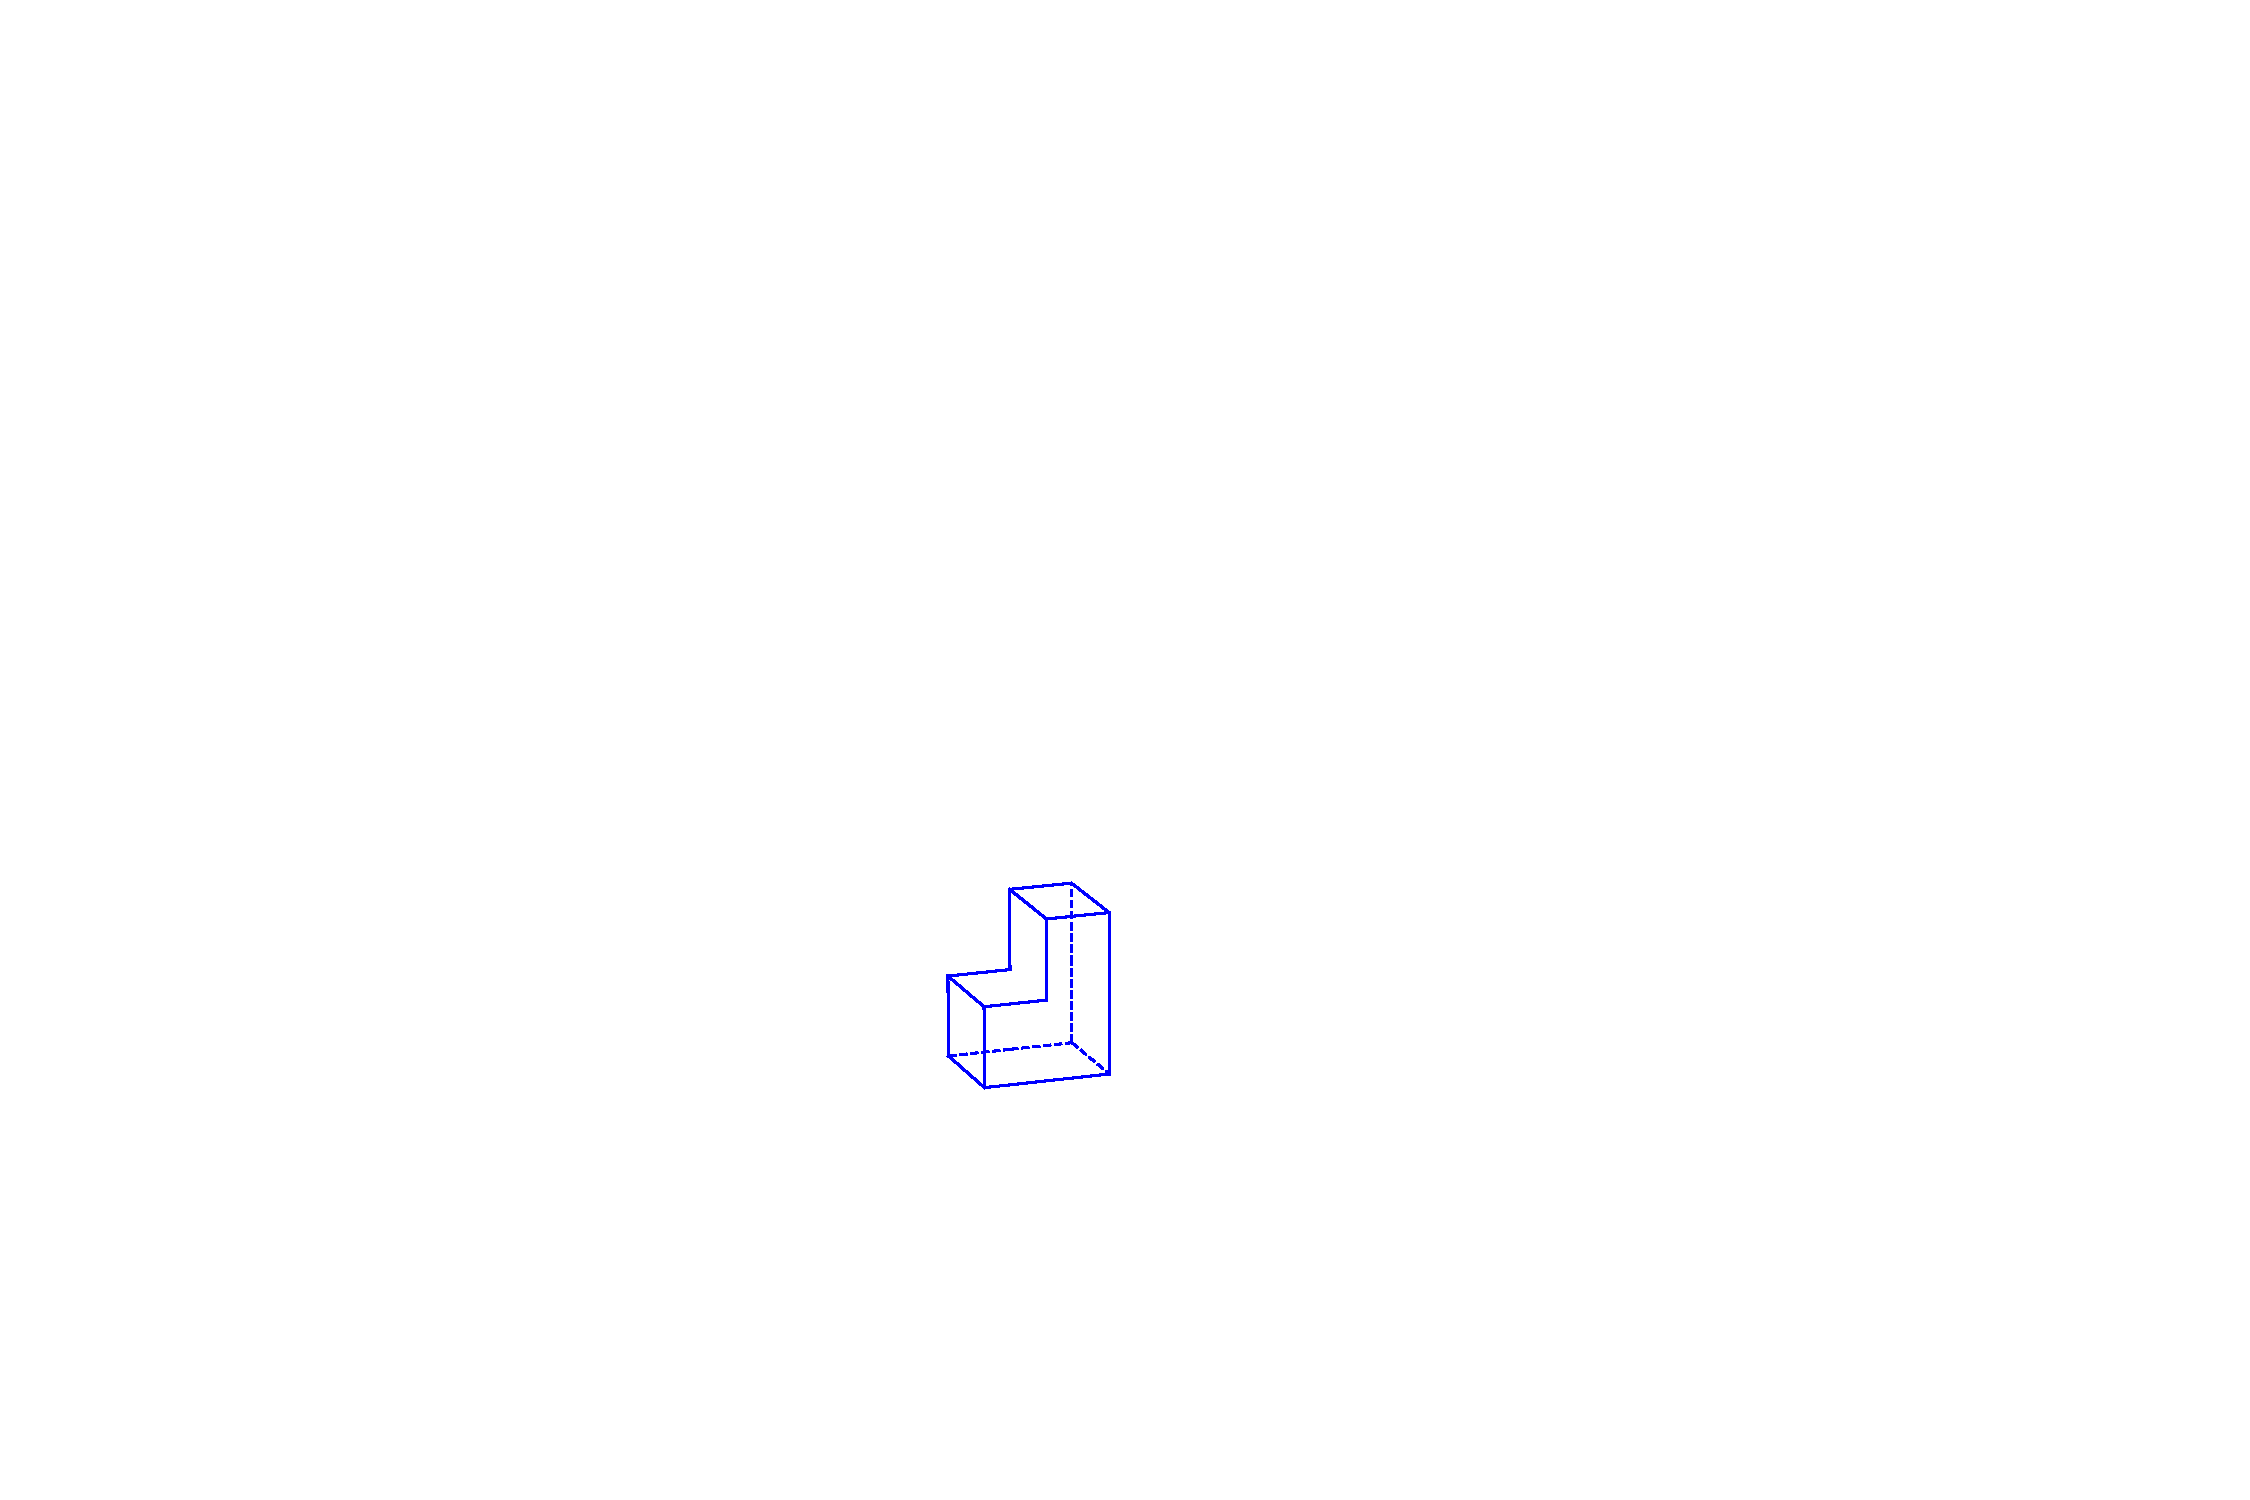
\includegraphics{Img/Kapitola4/CUBI.pdf}
            \caption{Sch\'{e}ma CUBIho s vyzna\v{c}en\'{y}mi rozm\v{e}ry.}
            \label{fig:CUBI}
        \end{figure}

        P\v{r}i implementaci tohoto experimentu byla pou\v{z}ita symerick\'{a} okrajov\'{a} podm\'{\i}nka \ref{sec:SymBouCon}. To bylo mo\v{z}n\'{e} prov\'{e}st z podstaty \'{u}lohy. Jeliko\v{z} je v\'{y}\v{s}ka p\v{r}ek\'{a}\v{z}ky v porovn\'{a}n\'{i} s v\'{y}\v{s}kou tunelu mal\'{a}, proud\v{e}n\'{\i} ve vrchn\'{i} polovin\v{e} tunelu se st\'{a}v\'{a} lamin\'{a}rn\'{i}m a tud\'{i}\v{z} pro n\'{a}s nezaj\'{i}mav\'{y}m.

        Velkou v\'{y}hodou pou\v{z}it\'{i} t\'{e}to okrajov\'{e} podm\'{i}nky je u\v{s}et\v{r}en\'{i} poloviny pam\v{e}ti, co\v{z} n\'{a}m umo\v{z}n\'{i} dohs\'{a}hnout jemn\v{e}j\v{s}\'{i}ho rozli\v{s}en\'{i}. 


        P\v{r}edm\v{e}tem z\'{a}jmu pro n\'{a}s bude rychlostn\'{i} a teplotn\'{i} profil t\v{e}sn\v{e} nad povrchem spodn\'{i} st\v{e}ny v\'{y}po\v{c}etn\'{i} oblasti $\overline{\hat{\Omega}}$. Nastaven\'{i} v\'{y}po\v{c}etn\'{i} oblasti pro simulace bude jako na obr\'{a}zku \ref{fig:ProblCUBI_domain}.


        \begin{figure}[H]
            \centering
            \includegraphics[width=\textwidth]{Img/Kapitola4/CUBI_domain.pdf}
            \caption{Sch\'{e}ma v\'{y}po\v{c}etn\'{i} oblasti pro \'{u}lohu \ref{sub:ProbCUBI}.}
            \label{fig:CUBI_domain}
        \end{figure}

        \subsection{Experiment CUBI}
        \label{sub:ProbCUBI}

            \begin{tcolorbox}[colframe=blue, title = \'{U}loha \ref{sub:ProbCUBI}]
                                        
                Parametry \'{u}lohy:
                \begin{itemize}
                    \begin{multicols}{2}
                    \item $\Omega = (0;1{,}25 \; \mathrm{m}) \times (0;1 \; \mathrm{m}) \times (0;0{,}5 \; \mathrm{m})$,
                    \item $t \in \langle 0;0{,}1 \rangle \ \mathrm{s}$,
                    \item $\nu = 1{,}552 \cdot 10^{-5} \ \mathrm{m^2 \ s^{-1}}$,
                    \item $u_{in} = 1 \ \mathrm{m \ s^{-1}}$, 
                    \item $T_{ini,a} = 5 \ ^{\circ}\mathrm{C}$,
                    \item $T_{in} = 5 \ ^{\circ}\mathrm{C}$,
                    \item $T_{ini,b} = 5 \ ^{\circ}\mathrm{C}$,
                    \item $D_{a} = 2{,}239 \cdot 10^{-3} \ \mathrm{m^2 \ s^{-1}}$, 
                    \item $D_b = 9{,}700 \cdot 10^{-3} \ \mathrm{m^2 \ s^{-1}}$,
                    \item $\omega = 0{,}01 \  \mathrm{kg \ s^{-3} \ K^{-1}}$.
                    \end{multicols}
                \end{itemize}
                
                Po\v{c}\'{a}te\v{c}n\'{\i} a okrajov\'{e} podm\'{\i}nky:
                \begin{itemize}
                    \item V $\overline{\hat{\Omega}}$ nastav\'{\i}me po\v{c}\'{a}te\v{c}n\'{\i} podm\'{\i}nky dle sekc\'{\i} \ref{sec:NSEIniCon} a \ref{sec:ADEIniCon}.
                    \item Na \v{c}\'{a}sti hranice $\hat{\Gamma}_{in}$ zvol\'{\i}me vstupn\'{\i} okrajov\'{e} podm\'{\i}nky popsan\'{e} v \ref{sec:NSEIniCon} a \ref{sec:ADEIniCon}.
                    \item Pro $\hat{\Gamma}_{out}$ vol\'{\i}me odtokov\'{e} podm\'{\i}nky dle \ref{sec:NSEIniCon} a \ref{sec:ADEIniCon}.
                    \item Na $\hat{\Gamma}_{w}$ pou\v{z}ijeme bounce-back okrajov\'{e} podm\'{\i}nky ze sekc\'{\i} \ref{sec:NSEIniCon} a \ref{sec:ADEIniCon}.
                    \item Na vrchn\'{i} st\v{e}nu $\hat{\Gamma}_{top}$ p\v{r}edep\'{i}\v{s}eme symetrickou okrajovou podm\'{i}nku \ref{sec:SymBouCon}. 
                    \item Pro t\v{e}leso $\overline{\hat{\Omega}}_b$ vol\'{\i}me n\'{a}sleduj\'{\i}c\'{\i} okrajov\'{e} podm\'{\i}nky: \begin{itemize}
                        \item Pro NSR sch\'{e}ma vol\'{\i}me na $\overline{\hat{\Omega}}_b$ bounce-back okrajovou podm\'{\i}nku dle \ref{sec:NSEIniCon},
                        \item V ADR sch\'{e}matu pou\v{z}ijeme na $\hat{\Gamma}_b$ p\v{r}estupovou podm\'{\i}nku, viz \ref{sec:ADEIniCon}.  
                    \end{itemize}
                \end{itemize}
                
                Parametry LBM:
                \begin{itemize}
                    \item $N_x \times N_y \times N_z \in \{ 40i \times 32i \times 16i\ | \ i \in \{ 3,4,\dots,25 \} \} $,
                    \item $\mathrm{Re} = 33 \ 333$,
                    \item $\nu_{LBM} = 10^{-4}$, odpov\'{\i}d\'{a} $\Delta t \approx 10^{-5} s$.
                \end{itemize}
            \end{tcolorbox}

        \subsection{V\'{y}sledky \'{u}lohy \ref{sub:ProbCUBI}}
        

        




\chapter*{Závěr}

\pagestyle{plain}

\addcontentsline{toc}{chapter}{Záv\v{e}r}

C\'{\i}lem t\'{e}to pr\'{a}ce bylo matematick\'{e} modelov\'{a}n\'{\i} izoterm\'{a}ln\'{\i}ho proud\v{e}n\'{\i} newtonovsk\'{e} nestla\v{c}iteln\'{e} tekutiny pomoc\'{\i} m\v{r}\'{\i}\v{z}kov\'{e} Boltzmannovy metody.

Prvn\'{\i} kapitola byla v\v{e}nov\'{a}na zasv\v{e}cen\'{\i} \v{c}ten\'{a}\v{r}e do matematick\'{e}ho modelu popisuj\'{\i}c\'{\i} rovnice izoterm\'{a}ln\'{\i}ho proud\v{e}n\'{\i}. V r\'{a}mci t\'{e}to kapitoly byly uvedeny rovnice popisuj\'{\i}c\'{\i} dynamiku tekutiny. 

Druh\'{a} kapitola se zam\v{e}\v{r}ovala na samotnou numerickou metodu pou\v{z}itou k simulac\'{\i} -- m\v{r}\'{\i}\v{z}kovou Boltzmannovu metodu (LBM). V t\'{e}to \v{c}\'{a}sti byla pops\'{a}na p\v{r}estupov\'{a} okrajov\'{a} podm\'{\i}nka, kter\'{a} byla v~r\'{a}mci pr\'{a}ce implementov\'{a}na. V t\'{e}to kapitole byly tak\'{e} pops\'{a}ny datov\'{e} struktury pou\v{z}it\'{e} v LBM k\'{o}du, d\'{a}le zde jsou uvedeny pozn\'{a}mky k implementaci na v\'{\i}ce grafick\'{y}ch kart\'{a}ch.  

Ve t\v{r}et\'{\i} kapitole jsou shrnuty v\'{y}sledky aplikace m\v{r}\'{\i}\v{z}kov\'{e} Boltzmannovy metody na \'{u}lohu formulovanou v prvn\'{\i} kapitole.  V prvn\'{\i} \v{c}\'{a}sti je \'{u}sp\v{e}\v{s}n\v{e} implementov\'{a}no pole pro prostorov\v{e} prom\v{e}nliv\'{y} difuzn\'{\i} koeficient. Druh\'{a} \v{c}\'{a}st se v\v{e}nuje implementaci p\v{r}estupov\'{e} okrajov\'{e} podm\'{\i}nky, kter\'{a} byla tak\'{e} \'{u}sp\v{e}\v{s}n\v{e} implementov\'{a}na. V posledn\'{\i} \v{c}\'{a}sti je LBM pou\v{z}ita k hled\'{a}n\'{\i} optim\'{a}ln\'{\i}ho rozm\v{e}ru radi\'{a}toru pro v\r{u}z FSE.12.

K numerick\'{y}m simulac\'{\i}m byl vyu\v{z}it k\'{o}d LBM vyu\v{z}\'{\i}vaj\'{\i}c\'{\i} softwarov\'{e}ho bal\'{\i}\v{c}ku CUDA od spole\v{c}nosti Nvidia, d\'{\i}ky kter\'{e}mu bylo umo\v{z}n\v{e}no po\v{c}\'{\i}t\'{a}n\'{\i} na grafick\'{y}ch kart\'{a}ch. Tento k\'{o}d je naps\'{a}n v jazyce C++ a ji\v{z} n\v{e}kolik let je vyv\'{\i}jen\'{y} na KM FJFI \v{C}VUT v Praze.  V r\'{a}mci t\'{e}to pr\'{a}ce byl v tomto k\'{o}du opraven model D3Q7. K\'{o}d byl pro \'{u}\v{c}ely pr\'{a}ce roz\v{s}\'{\i}\v{r}en o pole pro r\r{u}zn\'{e} difuzn\'{\i} koeficienty a tak\'{e} byla do k\'{o}du implementov\'{a}na p\v{r}estupov\'{a} okrajov\'{a} podm\'{\i}nka.

V bl\'{\i}zk\'{e} budoucnosti je c\'{\i}lem simulovat slo\v{z}it\v{e}j\v{s}\'{\i} geometrii chladi\v{c}e, kter\'{a} by m\v{e}la zohled\v{n}ovat i geometrii j\'{a}dra. D\'{a}le je v pl\'{a}nu porovnat v\'{y}sledky numerick\'{y}ch simulac\'{\i} s re\'{a}ln\'{y}mi daty ze senzor\r{u} vozu FSE.12. Dal\v{s}\'{\i}m c\'{\i}lem je studovat a vyhodnotit chov\'{a}n\'{\i} teplotn\'{\i}ho pole na mezn\'{\i} vrstv\v{e}.




% T\v{r}et\'{\i} kapitola byla v\v{e}nov\'{a}na samotn\'{y}m v\'{y}sledk\r{u}m testov\'{a}n\'{\i} implementace metody v\'{y}m\v{e}ny hybnosti. Z\'{\i}skan\'{a} s\'{\i}la vedla k v\'{y}po\v{c}tu bezrozm\v{e}rn\'{y}ch koeficient\r{u} odporu a vztlaku dan\'{e}ho t\v{e}lesa. Spr\'{a}vnost implementace v\'{y}po\v{c}tu s\'{\i}ly byla ov\v{e}\v{r}ov\'{a}na porovn\'{a}n\'{\i}m bezrozm\v{e}rn\'{y}ch koeficient\r{u} s referen\v{c}n\'{\i}mi hodnotami z \cite{schafer1996benchmark}. 

% K numerick\'{y}m simulac\'{\i}m byl vyu\v{z}\'{\i}v\'{a}n k\'{o}d LBM se softwarem CUDA od spole\v{c}nosti Nvidia umo\v{z}\v{n}uj\'{\i}c\'{\i}m paraleln\'{\i} v\'{y}po\v{c}et na grafick\'{y}ch kart\'{a}ch implementovan\'{y} v jazyce C++. Tento k\'{o}d je vyv\'{\i}jen na KM FJFI \v{C}VUT v Praze. Pro \'{u}\v{c}ely t\'{e}to pr\'{a}ce byl v tomto k\'{o}du implementov\'{a}n zmi\v{n}ovan\'{y} v\'{y}po\v{c}et s\'{\i}ly metodou v\'{y}m\v{e}ny hybnosti pro 2D a 3D model. Simulace \'{u}loh byly provedeny pro dv\v{e} r\r{u}zn\'{a} Reynoldsova \v{c}\'{\i}sla p\v{r}edstavuj\'{\i}c\'{\i} stabiln\'{\i} a nestabiln\'{\i} proud\v{e}n\'{\i}. Ve 2D \'{u}loze bylo p\v{r}ek\'{a}\v{z}kou t\v{e}leso kruhov\'{e}ho tvaru, ve 3D \'{u}loze byly za t\v{e}lesa voleny postupn\v{e} v\'{a}lec a kv\'{a}dr se \v{c}tvercovou podstavou.

% V bl\'{\i}zk\'{e} budoucnosti bude c\'{\i}lem roz\v{s}\'{\i}\v{r}it LBM k\'{o}d o rovnici veden\'{\i} tepla a simulovat v\'{y}m\v{e}n\'{\i}k tepla (nap\v{r}. chladi\v{c} v aut\v{e} nebo topen\'{\i} v m\'{\i}stnosti). V neposledn\'{\i} \v{r}ad\v{e} je v pl\'{a}nu implementovat dosud testovan\'{e} \'{u}lohy v softwaru OpenFOAM a porovnat s v\'{y}sledky LBM.



\bibliographystyle{plain}
\bibliography{reference}

\end{document}